\documentclass[upright, contnum]{umemoria}
\depto{Departamento de Ingeniería Eléctrica}
\author{Rodrigo Javier Pérez Dattari}
\title{Interactive Learning with Corrective Feedback for Continuous-Action Policies based on Deep Neural Networks}
\auspicio{Proyecto FONDECYT 1161500}
\date{2019}
\guia{Javier Ruiz del Solar}
\carrera{Magíster en Ciencias de la Ingeniería, Mención Eléctrica}
\carreraeng{Master of Engineering Sciences in Electrical Engineering}
\memoria{Tesis para optar al Grado de \break  Magíster en Ciencias de la Ingeniería, Mención Eléctrica\break \break
Memoria para optar al Título de Ingeniero Civil Eléctrico}
\comision{Javier Ruiz del Solar, Felipe Tobar, Nicolás Navarro-Guerrero}

\usepackage{lipsum}

\usepackage[utf8]{inputenc}
\usepackage[T1]{fontenc}
\usepackage{color}
\usepackage{titlesec}
\usepackage[noend]{algpseudocode}
\usepackage{amsmath}
\usepackage{algorithm}
\usepackage{subfig}
\usepackage{blindtext, graphicx}
\usepackage{color}
\definecolor{mygray}{RGB}{200, 200, 200}
\definecolor{mygreen}{RGB}{1, 200, 1}
\definecolor{lightgray}{gray}{0.8}
\definecolor{lightlightgray}{gray}{0.9}
\newcommand{\new}[1]{\color{blue}{#1}\color{black}}
\newcommand{\replace}[1]{\color{mygray}{#1}\color{black}} % replace text, or not needed
\newcommand{\remove}[1]{\color{red}{#1}\color{black}}
\newcommand{\comment}[1]{\color{mygreen}{#1}\color{black}}
\newcommand{\note}[1]{\color{red}\textbf{{#1}}\color{black}}

\titlespacing*{\section}{0pt}{\baselineskip}{\baselineskip}
\titlespacing*{\subsection}{0pt}{\baselineskip}{\baselineskip}
\titlespacing*{\subsubsection}{0pt}{\baselineskip}{\baselineskip}
\DeclareMathOperator*{\argmax}{arg\,max}
\DeclareMathOperator*{\argmin}{arg\,min}

\begin{document}

\frontmatter
\maketitle

\begin{abstract}
El Aprendizaje Reforzado Profundo (DRL) se ha transformado en una metodología poderosa para resolver problemas complejos de toma de decisión secuencial. Sin embargo, el DRL tiene varias limitaciones cuando es usado en problemas del mundo real (p.ej. aplicaciones de robótica). Por ejemplo, largos tiempos de entrenamiento (que no se pueden acelerar) son requeridos, en contraste con ambientes simulados, y las funciones de recompensa pueden ser difíciles de especificar/modelar y/o computar. Más aún, el traspaso de políticas aprendidas en simulaciones al mundo real no es directo ("reality gap"). Por otro lado, métodos de aprendizaje de máquinas basados en la transferencia de conocimiento humano a un agente han mostrado ser capaces de obtener políticas con buenos desempeños sin necesariamente requerir el uso de una función de recompensa, siendo eficientes en lo que respecta al tiempo.

En este contexto, en esta tesis se introduce una estrategia de Aprendizaje Interactivo de Máquinas (IML) para entrenar políticas modeladas como Redes Neuronales Profundas (DNNs), basada en retroalimentación correctiva humana con un método llamado D-COACH. Se combina Aprendizaje Profundo (DL) con el método Asesoramiento Correctivo Comunicado por Humanos (COACH), en donde humanos no expertos pueden entrenar políticas corrigiendo las acciones que va tomando el agente en ejecución. El método D-COACH tiene el potencial de resolver problemas complejos sin necesitar de muchos datos o tiempo. Resultados experimentales validan la eficiencia del método propuesto en plataformas simuladas y del mundo real, en espacios de estados de baja y alta dimensionalidad, mostrando la capacidad de aprender políticas en espacios de acción continuos de manera efectiva.

El método propuesto mostró resultados particularmente interesantes cuando políticas parametrizadas con Redes Neuronales Convolucionales (CNNs) fueron usadas para resolver problemas con espacios de estado de alta dimensionalidad, como pixeles desde una imagen. Al usar CNNs, los agentes tienen la capacidad de construir valiosas representaciones del estado del ambiente sin la necesidad de hacer ingeniería de características por el lado del diseñador (lo que era siempre necesario en el Aprendizaje Reforzado (RL) clásico). Estas propiedades pueden ser muy útiles en robótica, ya que es común encontrar aplicaciones en donde la información adquirida por los sensores del sistema es de alta dimensionalidad, como imágenes RGB. Darles la habilidad a los robots de aprender desde datos del alta dimensionalidad va a permitir aumentar la complejidad de los problemas que estos pueden resolver.

A lo largo de esta tesis se proponen y validan tres variaciones de D-COACH. La primera introduce una estructura general para resolver problemas de estado de baja y alta dimensionalidad. La segunda propone una variación del primer método propuesto para problemas de estado de alta dimensionalidad, reduciendo el tiempo y esfuerzo de un humano al entrenar una política. Y por último, la tercera introduce el uso de Redes Neuronales Recurrentes para añadirle memoria a los agentes en problemas con observabilidad parcial.

\end{abstract}

\begin{abstract_eng}
Deep Reinforcement Learning (DRL) has become a powerful methodology to solve complex decision making problems. However, DRL has several limitations when used in real-world problems (e.g., robotics applications). For instance, long training times (that cannot be accelerated) are required in contrast to simulated environments, and reward functions may be hard to specify/model and/or to compute. Moreover, the transfer of policies learned in a simulator to the real-world has limitations (reality gap). On the other hand, machine learning methods that rely on the transfer of human knowledge to an agent have shown to be time efficient for obtaining well performing policies and do not require a reward function.

In this context, this thesis proposes an alternative Interactive Machine Learning (IML) strategy for training Deep Neural Network (DNN) policies based on human corrective feedback, with a method called Deep COACH (D-COACH). Deep Learning is combined with the COrrective Advice Communicated by Humans (COACH) framework, in which non-expert humans shape policies by correcting the agent’s actions during execution. The D-COACH framework has the potential to solve complex problems without much data or time required. Experimental results validated the efficiency of the proposed framework in simulated and real-world platforms, with state spaces of low and high dimensionality, showing the capacity to successfully learn policies for continuous action spaces. 

The proposed framework showed particularly interesting results when learning policies parameterized with Convolutional Neural Networks (CNNs) for high-dimensional state spaces, such as raw pixels from an image. By using CNNs, agents are given the possibility to build rich state representations of the environment without feature engineering on the side of the designer (which was always necessary in classical RL). These properties can be very useful in robotics, since it is common to find applications with high-dimensional observations, such as RGB images. Giving robots the ability to learn from such high-dimensional data will allow to scale up the complexity of what robots are able to do.

In this thesis three variations of D-COACH are proposed and validated. The first one introduces a general structure for solving problems with low-dimensional and high-dimensional state spaces. The second one proposes a variation of the first approach for high-dimensional state problems, reducing the time and effort of a human for training a policy. And finally, the third variation introduces the use of Recurrent Neural Networks for adding memory to agents in problems with partial observability.
\end{abstract_eng}


\begin{dedicatoria}
A mi abuelo Ernesto
\end{dedicatoria}

\begin{thanks}

\end{thanks}

\cleardoublepage
\tableofcontents
\cleardoublepage
\listoftables
\cleardoublepage
\listoffigures

\mainmatter

\chapter{Introduction}
\section{Motivation and Problem Statement}
In  recent years, outstanding results in complex decision-making problems have been obtained with Deep Reinforcement Learning (DRL). State-of-the-art algorithms have solved problems with large state-action spaces, such as playing Atari games \cite{atari}, beating the world champion in GO \cite{Silver2016} or defeating a top professional player in StarCraft II \cite{alphastarblog}, along with low level simulated continuous control tasks in environments such as the ones included in the OpenAI Gym \cite{brockman2016openai} and the DeepMind Control Suite \cite{tassa2018deepmind}. 

Nevertheless, in robotic problems, DRL is still limited in applications with real-world problems \cite{Gu2017}. Most of the tasks that have been successfully addressed with DRL have two common characteristics: 1) they have well-specified reward functions, and 2) they require large amounts of trials, which means long training periods (or powerful computers) to obtain a satisfying behavior. These two characteristics can be problematic in cases where 1) the goals of the tasks are poorly defined or hard to specify/model (reward function does not exist), 2) the execution of many trials is not feasible (real systems case) and/or not much computational power or time is available, and 3) sometimes additional external perception is necessary for computing the reward/cost function.

In this regard, the transfer of knowledge learned in a simulator to the real-world is a typical solution. However, the mismatch between the virtual and real environment, known as ``Reality Gap``, is often problematic \cite{koos2013transferability}. This results in agents that do not perform at their best in the real-world. Thus, it would be preferable to learn/fine-tune policies directly in the real-world.

In contrast, Machine Learning methods that rely on transfer of human knowledge, Interactive Machine Learning (IML) methods, have shown to be time efficient for obtaining good performance policies and may not require a well-specified reward function; moreover, some methods do not need expert human teachers for training high performance agents \cite{akrour2011preference,Knox:2009:ISA:1597735.1597738,Celemin2018AnInteractive}. In previous years, IML techniques were limited to work with low-dimensional state spaces problems and to the use of function approximation such as linear models of basis functions (choosing a right basis function set was crucial for successful learning), in the same way as Reinforcement Learning (RL). But, as DRL have showed, by approximating policies with Deep Neural Networks (DNNs) it is possible to solve problems with high-dimensional state spaces, without the need of feature engineering for preprocessing the states. If the same approach is used in IML, the DRL shortcomings mentioned before can be addressed with the support of human users who participate in the learning process of the agent.

Therefore, in this work we study the use of human corrective feedback during task execution to learn DNN policies in state spaces of low and high dimensionality in continuous action problems (which is the case for most of the problems in robotics).

In this context, this thesis proposes an alternative Interactive Machine Learning strategy for training Deep Neural Network policies based on human corrective feedback, with a method called Deep COACH (D-COACH). Deep Learning is combined with the COrrective Advice Communicated by Humans (COACH) framework, in which non-expert humans shape policies by correcting the agent’s actions during execution. The D-COACH framework has the potential to solve complex problems without much data or time required. Experimental results validated the efficiency of the proposed framework in simulated and real-world platforms, with state spaces of low and high dimensionality, showing the capacity to successfully learn policies for continuous action spaces. 

Three variations of D-COACH are introduced:

\begin{enumerate}
    \item \textbf{Offline state representation learning (D-COACH)}
    \item \textbf{ONline state representation learning (D-COACH ON)}
    \item \textbf{Memoryful ONline state representation learning (D-COACH MON)}
\end{enumerate}

D-COACH and D-COACH ON assume that the agents interact in fully-observable environments. As a consequence, they make decisions solely based on what they are observing on that precise moment. There is no difference between these two approaches in problems with low-dimensional states. A fully connected network policy is interactively trained during task execution with human corrective feedback. Nevertheless, in high-dimensional state problems D-COACH ON enhances the methodology proposed in D-COACH. In both approaches a convolutional autoencoder is added to the network architecture for state dimensionality reduction. In the D-COACH formulation, a demonstration session is required at the beginning of the training process for tuning the weights of the autoencoder. After that, a fully connected network policy is linked to the output of the encoder layers (latent space of the autoencoder), and is trained interactively, in the same way as in the low-dimensional state case. In contrast, D-COACH ON eliminates the need of demonstration sessions and trains the policy and the autoencoder simultaneously, sharing the convolutional layers (encoder) between both networks. This reduces the time and effort of the human for teaching a policy.

D-COACH MON assumes that the agents interact in partially-observable environments, which is true in many real-world scenarios, and tries to cover a subset of these problems. Memory is added to the agents by using recurrent layers in the network architectures in order to obtain well performing policies in problems where past observations contain crucial information about the current state of the agent. As in D-COACH ON, everything is learned online, without the need of a demonstration session. 

Throughout this thesis, we give special emphasis to studying the use of policies parameterized with Convolutional Neural Networks (CNNs) for solving problems with high-dimensional state spaces, such as raw pixels from an image. CNNs give agents the possibility to build rich state representations of the environment without feature engineering on the side of the designer (which was always necessary in classical RL). These properties can be very useful in robotics, since it is common to find applications with high-dimensional observations, such as RGB images. Giving robots the ability to learn from such high-dimensional data will allow to scale up the complexity of what robots are able to do. All of the proposed variations of D-COACH have as common denominator the study of CNNs,  seeking to exploit their properties in the best possible way. 

\section{Objectives}
\subsection{General Objective}
The general objective of this thesis is to develop and validate an algorithm that exploits the advantages of combining deep learning with human corrective feedback for learning policies when solving sequential decision-making problems in robotics. 

\subsection{Specific Objectives}

\begin{itemize}
    \item Study the state-of-the-art of robot learning algorithms for solving sequential decision-making problems.
    \item Propose and implement an algorithm that, by using deep neural networks policies, allows robots to learn to solve tasks in continuous-action domains from low-dimensional and high-dimensional states using online human corrective feedback. 
    \item Validate the proposed algorithm with tasks using simulated and real platforms.
    \item Propose and validate a variation of the algorithm to solve problems with partially observed environments.
\end{itemize}

\section{Hypothesis}
Human corrective feedback can be used to learn well performing deep neural network policies. As a consequence, an algorithm of this kind will effectively inherit the learning properties of using human corrective feedback and the function approximation properties of deep neural networks. Combining both approaches will result in a time-efficient and reward function free learning algorithm capable of solving problems using complex observations, such as raw pixels from an image.

\section{Outline}
This thesis is divided in six chapters.

\begin{itemize}
    \item \textbf{Chapter 2} presents the theoretical framework of this work. Both the areas of sequential decision-making and deep learning are revised in order to use them as baselines for the development of the thesis.
    \item \textbf{Chapter 3} introduces D-COACH. The ideas taken from the COACH framework are discussed and the formulation of D-COACH is presented. This approach is validated using simulated and real-world platforms.
    \item \textbf{Chapter 4} proposes an enhanced variation of D-COACH introduced in Chapter 2 (D-COACH ON), tackling one of its main shortcomings. This new version of the algorithm is able to learn policies from scratch in problems with high-dimensional state spaces in one learning step, while the previous version of D-COACH had an extra offline learning step.
    \item \textbf{Chapter 5} introduces a variation of D-COACH that adds memory to the agents (D-COACH MON) in order for them to solve tasks in partially observable environments. In contrast, Chapters 3 and 4 assume that the environments are fully observable, which is not true in many real-world scenarios.
    \item \textbf{Chapter 6} gathers the conclusions and the future work of this thesis.
\end{itemize}
\chapter{Theoretical Framework}
\section{Machine Learning}

Machine Learning (ML) is a discipline that studies ways of finding patterns in data by learning from experience. What this mean, is that an algorithm in charge of accomplishing an specific task is able to progressively improve its performance (learn) by comparing its output with data (experience) in a way that indicates how good/bad is doing. If the algorithm is doing good, then the learning process is finished. If is not doing so good, then the algorithm updates its parameters to match (if possible) its output with what is expected.   
\subsection{Deep Learning}

\subsubsection{Autoencoder}

\section{Policy Learning}
\note{POLICY DESCRIPTION}
\subsection{Reinforcement Learning}
\subsubsection{Deep Reinforcement Learning}
\subsection{Learning from Demonstration}
\subsubsection{The Correspondence Problem}
\subsection{Interactive Learning}
\subsubsection{Evaluative Feedback}
\subsubsection{Corrective Feedback}
\section{Function Approximation}
\subsection{Linear Model of Basis Functions}
\subsection{Artificial Neural Networks}
\section{COrrective Advice Communicated by Humans (COACH)}
\chapter{Introducing Deep Neural Networks into the COACH Framework}
In this chapter, we propose to extend the use of human corrective feedback during task execution to learn policies with state spaces of low and high dimensionality in $\text{continuous-action}$ problems (which is the case for most of the problems in robotics) using deep neural networks.

 We combine Deep Learning (DL) with the corrective advice based learning framework called COrrective Advice Communicated by Humans (COACH) \cite{Celemin2018AnInteractive}, thus creating the Deep COACH (D-COACH) framework. In this approach, no reward functions are needed and the amount of learning episodes is significantly reduced in comparison to alternative Reinforcement Learning (RL) approaches.

\section{Overview}
In previous years, learning algorithms for solving sequential decision-making problems heavily relied on carefully handcrafted features based on human intuition and knowledge about them to obtain good performances. Also, when using linear combination of basis functions (LCBFs) as function approximator, which was one of the most commonly used function approximator, for each problem it was necessary to select a specific set of basis functions. Choosing a well performing set of basis functions is a process that may require expert knowledge or several tests, which may become very time consuming or unfeasible as the size of the $\text{state-action}$ space increases. This is also a consequence of the \emph{Curse of Dimensionality} \cite{Bellman1957} which states that as the number of the dimensions of a space grows (state and/or action spaces in this case), exponentially more data and computation are needed to completely cover it. In LCBFs, this often means that their number of parameters $\theta$ grows exponentially as the number of dimensions increase. As a consequence, for most of the cases, learning algorithms needed handcrafted features in low-dimensional state spaces to adequately converge.

Given that COACH uses LCBFs as function approximator, it does not scale up well to problems with high-dimensional state spaces. However, the ideas proposed in COACH for shaping policies are independent of the function approximator that is used. With nowadays techniques, it has been shown that by approximating policies with Deep Neural Networks (DNNs) it is possible to solve problems with high-dimensional state spaces and with unprocessed raw information. So it seems as a natural step to extrapolate the ideas proposed in COACH to DNNs. 

\section{Methodology}
COACH is an algorithm designed to work with LCBFs that has different versions and variations. Consequently, in order to extrapolate its ideas to DNNs, it is necessary to see which of those can be used and why.

Given that in this thesis we are introducing the first approach that combines COACH with DNNs, we decided to design an algorithm based on the basic structure of COACH, shown in Algorithm \ref{algorithm:COACH} (Chapter \ref{sss:COACH}). We believe that there is still space to incorporate more ideas into D-COACH using the work presented in this thesis as a baseline.

The basic structure of COACH proposes two main ideas:

\begin{enumerate}
    \item \textbf{Using corrective feedback to shape policies:} COACH was built from this idea, so it is not possible not to consider it. D-COACH uses corrective feedback \emph{almost} exactly as COACH. In COACH, it is proposed that each dimension of the action space should be trained independently, which has the advantage of creating a working framework that does not need any prior information about the problem in order to give corrections. We call this type of policy updating \emph{decoupled} training, so a correction in an specific action dimension does not modify the magnitude of the actions in other axes for the same corresponding state. However, in this work we consider that for some problems it may be advantageous to exploit prior user knowledge about relations between the different dimensions of the actions. In this way, a correction in one of the action axes may be used to update more than one dimension. We call this case \emph{coupled} training.
    
    \item \textbf{Using past corrections to modify the effects of newer ones:} In COACH, this idea is reflected in the Human Model; in D-COACH, a replay buffer (or experience replay, see Chapter \ref{sss:ER}) is incorporated into the algorithm, which is a technique that has been strongly validated with several DRL approaches \cite{atari, haarnoja2018soft, Lillicrap2015}. Even though both the Human Model and the replay buffer use information given by past corrections to modify the effects of newer ones, they do not do it in the same way. The Human Model modifies the learning rate of the policy adaptively; the replay buffer updates the policy constantly by replaying past corrections. Including a Human Model into $\text{D-COACH}$ could help with the dilemma of setting either a too large or too small learning rate for updating the weights of a policy. In this case, we did not include a Human Model because this would have meant to add a second DNN model in charge of learning it. Thus, the overhead of D-COACH would have increased and we prioritized a lighter framework.
\end{enumerate}


\subsection{Low-Dimensional vs High-dimensional States}
When using DNNs, problems are often separated depending on the nature of their network inputs. When these inputs are processed data (such as handcrafted features in RL) a common approach is to use FNNs; When they are unprocessed raw information, CNNs are the most common option. In the RL context, given that the input of the networks is the state/observation of the environment, we use the term \emph{low-dimensional states} to refer to the input of the former, and \emph{high-dimensional states} to refer to the input of the later. Thus, FNNs are used in problems with low-dimensional state spaces and CNNs in problems with high-dimensional state spaces. Nevertheless, it is important to notice that handcrafted features are not necessarily low-dimensional and that FNNs may be also used in those cases. This is a commonly made association because the input of classic RL approaches were handcrafted features whose size was limited by the curse of dimensionality (and the computational power available at that time), and, as a consequence, they were low-dimensional.

Training CNN policies is a more challenging problem than training FNN policies. Both the state representation from raw data (this work focuses on applications with raw images as observation) and the policy must be learned from information interactively given by a human. DNNs have shown to need large sets of data and experience to adequately converge in complex problems, such as those with $\text{high-dimensional}$ inputs. The requirement of massive amounts of trials can be problematic because human users cannot keep on assisting the training for a long time due to stress, fatigue, or other factors that may lead to a lack of concentration.

To address this limitation, we employ \emph{state representation strategies} in problems with high-dimensional states/observations. The convolutional layers of a CNN can be interpreted as operations that extract the most relevant features out of a high-dimensional input. Thus, the output of these layers (which is commonly linked to a FNN in regression problems) can be seen as a representation of the state in a new space where the problem is easier to solve. This is what we call the state representation. So, in this context, state representation strategies refer to techniques employed for assisting the learning process of the state representation. In this work, the state representation of the policy is trained with additional criteria, adding an autoencoder to help with the training of the convolutional layers (or encoding layers) of the network.

\subsubsection{Offline State Representation Learning}
The D-COACH version introduced in this Chapter proposes to learn policies in a 3-step sequential process. In the first step, a session of demonstrations where observations of the environments are captured is recorded. Then, in a second step, the convolutional layers of the policy/autoencoder are trained with the recorded data, while tuning an  autoencoder  used  for state representation of reduced dimensionality, (Figure \ref{fig:ms}(a)). The state is embedded in the latent space of an autoencoder. Finally, in the third step, the convolutional layers of the trained encoder are frozen, then the subsequent non-convolutional layers (right hand side of Figure \ref{fig:ms}(b)) are trained interactively based on the corrections that the teacher advises to the agent. Figure \ref{fig:ms} depicts the second and third steps of this strategy. This kind of sequential strategy has been proven to work in decision-making problems \cite{Warnell2017,Finn2015,Ha2018}.

\begin{figure}[h]
\centering
\subfloat[][Autoencoder network for learning the state representation of the policy based on the demonstrations database.]{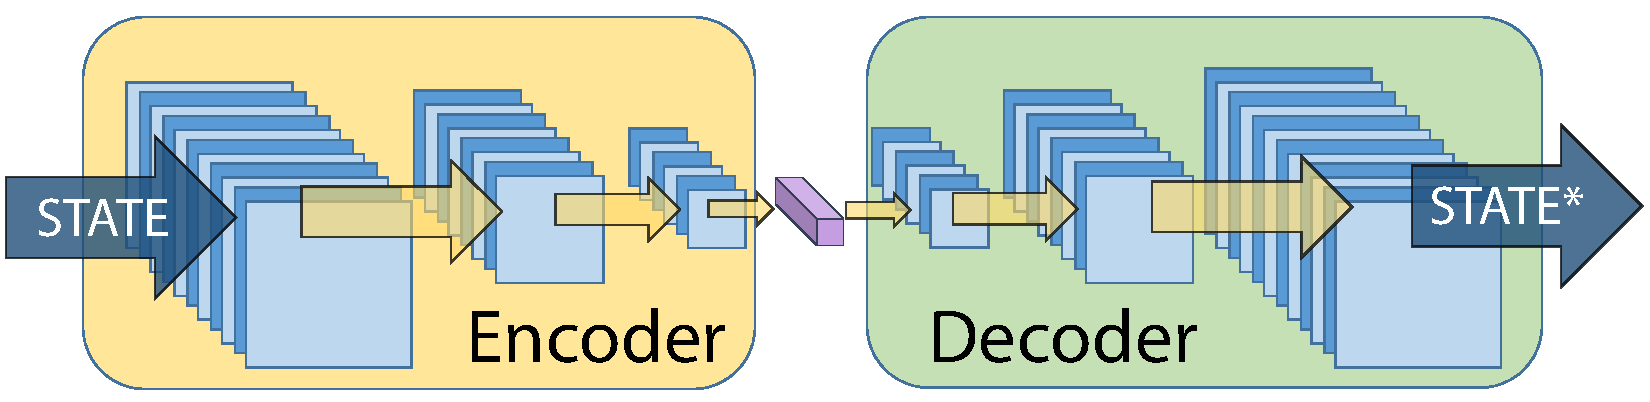
\includegraphics[width=0.45\linewidth]{imagenes/cap2/m1_p1.pdf}}
\hspace{0.1cm}
\subfloat[][Interactive training of the policy using the trained convolutional layers.]{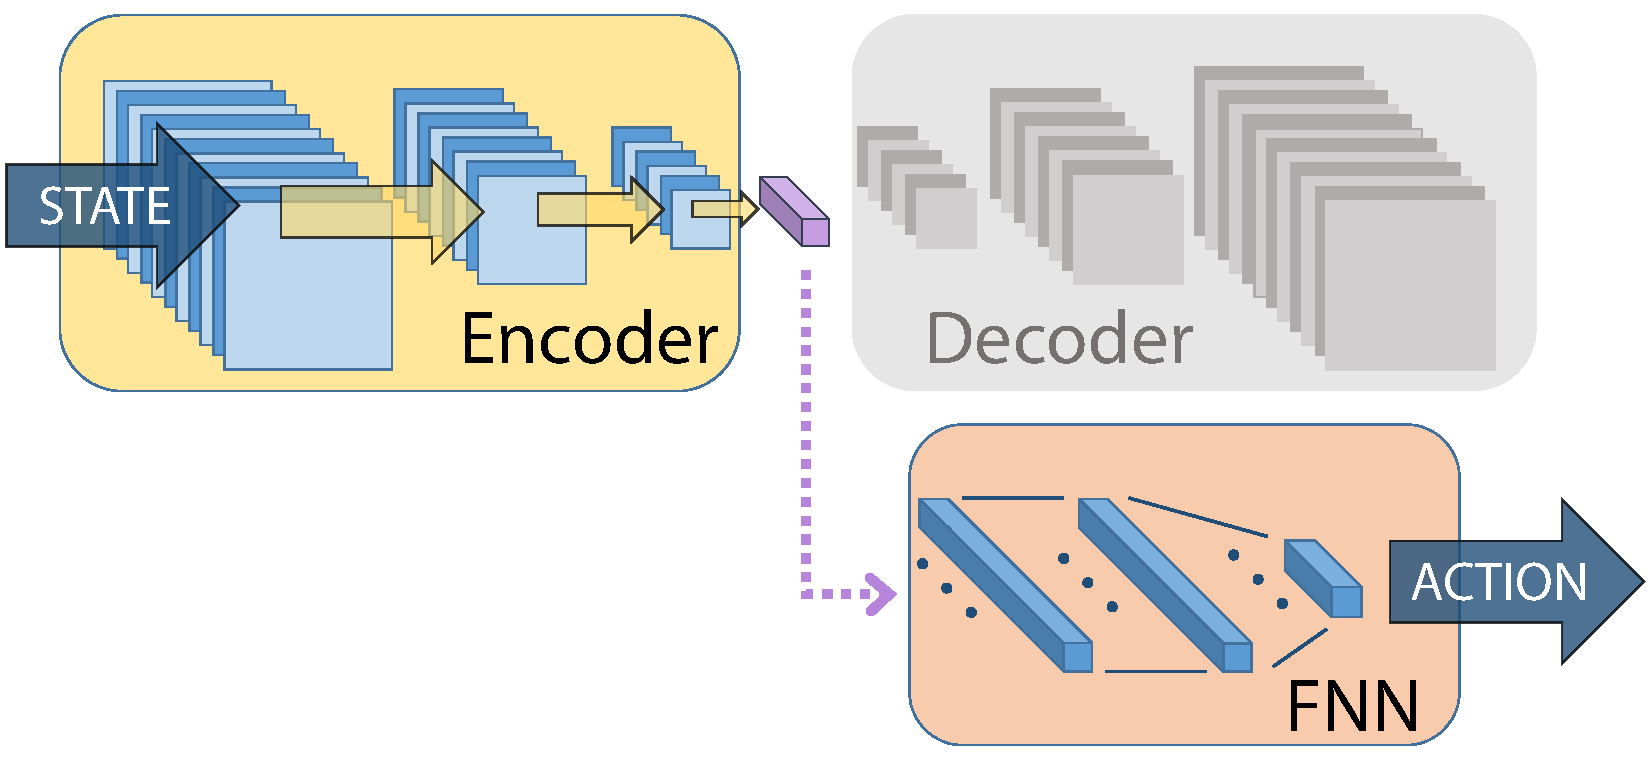
\includegraphics[width=0.45\linewidth]{imagenes/cap2/m1_p2.pdf}}
\caption{D-COACH offline state representation learning.} 
\label{fig:ms} 
\end{figure}

In the case of low-dimensional state problems, the state is fed into a FNN, skipping the autoencoder related steps and training the policy with interactive feedback directly. Figure \ref{fig:network_diagram} summarizes the network architecture for both low-dimensional and high-dimensional state problems.

\begin{figure}[h]
    \centering
    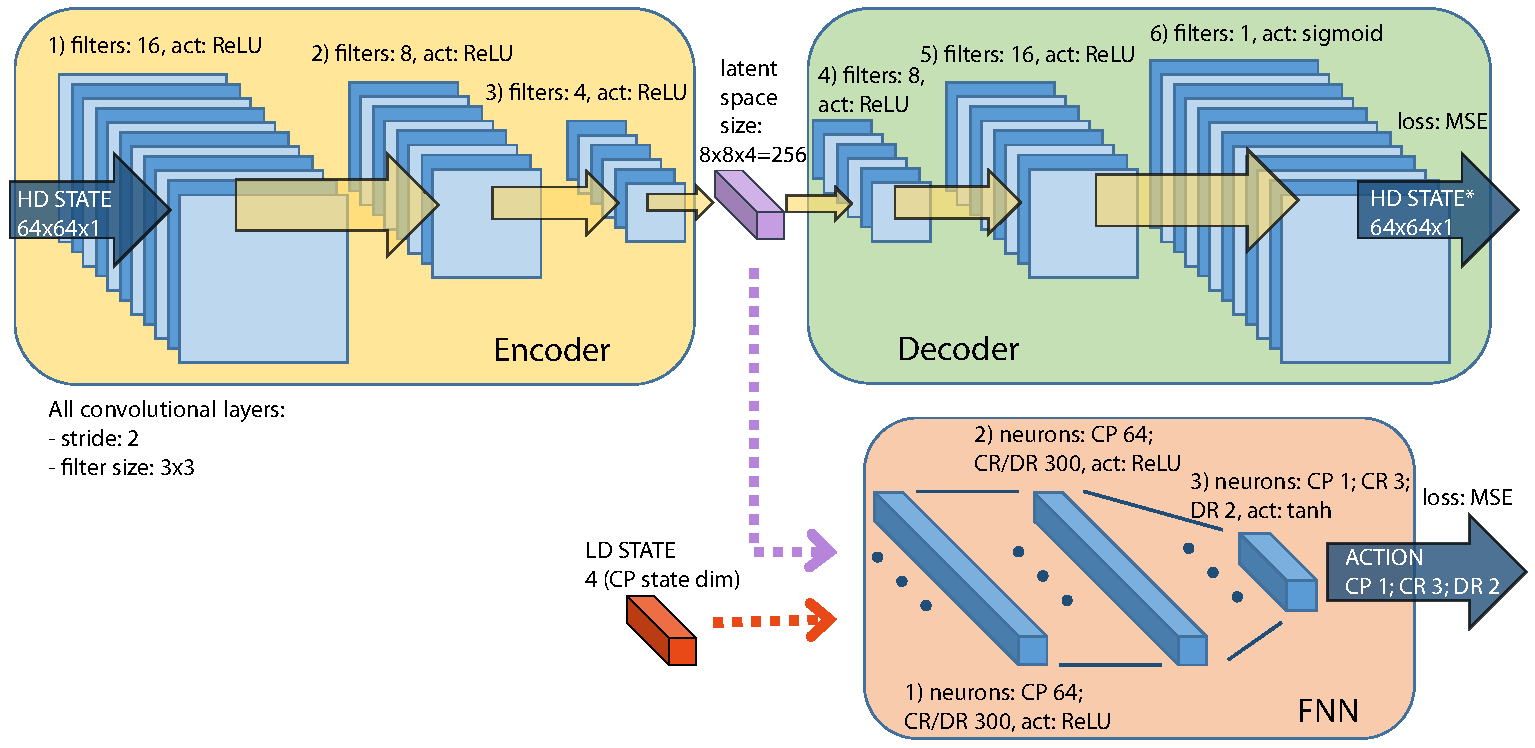
\includegraphics[width=0.9\linewidth]{imagenes/cap2/ISER_diagram.pdf}
    \caption{D-COACH neural networks architecture. HD STATE: high-dimensional state space, input of FNN is the latent space of the autoencoder (purple arrow). LD STATE: low-dimensional state space, input of FNN is the observed state (red arrow). Variations between environments are specified with the acronyms CP (Cart-Pole), CR (Car Racing) and DR (Duckie Racing). }
    \label{fig:network_diagram}
\end{figure}

\subsection{The Algorithm}
In D-COACH v1, the policies are updated every time feedback is received and also by sampling from a memory buffer $\mathcal{B}$ with a fixed frequency every $b$ time steps. Every time the user advises a correction, the buffer $\mathcal{B}$ is fed with the current state and a label generated by adding the action taken with the error correction $y_{label}=a+\mathit{error}$.

The high-dimensional case can be seen as an extension of the low-dimensional case, where an offline state learning process must be added. Algorithm \ref{algorithm:DeepCOACH} presents the D-COACH v1 pseudocode.

\begin{algorithm}[h]
\caption{D-COACH v1: Offline State Representation Learning}\label{algorithm:DeepCOACH}
\begin{algorithmic}[1]
\State \textbf{Require:} error magnitude $e$, buffer update interval $b$, buffer sampling size $N$, buffer min. size $k$, buffer max. size $K$, pre-trained encoder parameters (if convolutional) 
\State \textbf{Init:} $\mathcal{B} = []$  \emph{\# initialize memory buffer}
\For{t = 1,2,...}{}
\State \textbf{observe} state $s_{t}$
\State \textbf{execute} action $a_{t}=\pi(s_{t})$
\State \textbf{feedback} human corrective advice $h_{t}$
\If{$h_{t}$ is not \textbf{0}}
\State $\mathit{error}_{t} = h_{t}\cdot e$
\State $y_{label(t)} = a_{t} + \mathit{error}_{t}$ 
\State \textbf{update} $\pi(s)$ using SGD with pair ($s_{t}$, $y_{\mathit{label}(t)}$) 
\State \textbf{update} $\pi(s)$ using SGD with a mini-batch sampled from $\mathcal{B}$
\State \textbf{append} $(s_{t}, y_{\mathit{label}(t)})$ to $B$
\If{length($\mathcal{B}$) $> K$ }
\State $\mathcal{B} = \mathcal{B}[2:K+1]$
\EndIf
\EndIf
\If{mod(t, b) is 0 and length($\mathcal{B}$) $\geq k$}
\State \textbf{update} $\pi(s)$ using SGD with a mini-batch sampled from $\mathcal{B}$
\EndIf
\EndFor
\end{algorithmic}
\end{algorithm}

\section{Experiments and Results}
%\textbf{Even though COACH works well in low-dimensional state problems, the set of basis functions used in the LCBF must be selected independently for every problem. In some cases this could be time consuming or tedious. This engineering step is not necessary when using DNNs; thus, the same DNN architecture could be reused in different problems, saving time to the designers/engineers.}

Our proposed algorithm is validated experimentally in three different problems: 

\textbf{(i) Cart-Pole:} A simulated task with low-dimensional state space where the objective is to balance a pole attached to a cart. The cart can only move in one axis with an acceleration value between $-1$ and $1$. The state has four dimensions, which consists of the position $x$ and velocity $\dot x$ of the cart, and the angle $\theta$ and angular velocity $\dot \theta$ of the pole.

\textbf{(ii) Car Racing:} A simulated problem (from OpenAI gym \cite{brockman2016openai}) in which the agent has to learn to drive from a top-down view of a racing car game (see Fig.~\ref{fig:Car_Racing}). The objective of the task is to drive a racetrack as fast as possible without leaving it. The default state that is given by the environment is a $96\times96\times3$ top-down view of the car which we downsampled to $64\times64\times1$. The continuous-action space consists of 3 dimensions: \textbf{[direction, acceleration, brake]}. The \emph{direction} range goes from $-1$ to $1$, the \emph{acceleration} from $0$ to $1$ and the \emph{brake} from $0$ to $1$.

\begin{figure}[h]
    \centering
    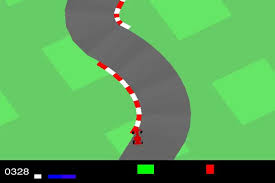
\includegraphics[scale=0.8]{imagenes/cap3/car_racing_env.jpg}
    \caption{Car Racing, environment view.}
    \label{fig:Car_Racing}
\end{figure}

\textbf{(iii) Duckie Racing:} This is also a driving task with high-dimensional input, but in this case with a real robot, which has an onboard camera that gives a first-person view of the environment. The robot consist of a Duckiebot from the project Duckietown \cite{Paull2017}. A $120\times160\times3$ observation image is received from the environment which is downsampled to $64\times64\times1$. The duckiebot is a differential robot, so the default actions consisted of speed commands ranging from -1 to 1 for each of the two wheels. To make it more intuitive for a human teacher to give feedback, the environment had an inverse kinematics module for the actions to be linear and rotational speeds instead, also ranging from -1 to 1. This problem is also used for experiments and validation with simulated and real human teachers.

The experiments with the simulated agents are intended to compare the complete D-COACH v1 presented in Algorithm \ref{algorithm:DeepCOACH}, along with a version of it without replay buffer (ignoring lines 2 and 11-16), and with a well known DRL agent (Deep Deterministic Policy Gradient DDPG \cite{Lillicrap2015} implemented by OpenAI \cite{baselines}). The comparison is carried out by plotting the cumulative reward obtained at each episode by the agent as a function of time. In the case of $\text{D-COACH}$ v1, the obtained reward is only used as a performance metric. Also, the results are presented as a function of time instead of episodes (except in the Duckie Racing experiment), because episodes can have variable duration depending on the policy. Hence, the episode scale would not properly show the time taken by the learning process, which is an important characteristic, since $\text{D-COACH}$ v1 is meant to work with real robots. The simulated environments, Cart-Pole and Car Racing, were ran at $22.5$ and $20.5$ FPS, respectively. These experiments were carried out using human teachers and simulated teachers. Humans had approximately 5 minutes to practice teaching in each environment. The learning curves of agents trained by 10 human teachers were obtained and averaged; the learning curves of agents trained by a simulated teacher were repeated 30 times and averaged. Along with the algebraic mean, the confidence intervals that represent the $60^{th}$ percentile of the data were plotted. In the case of the Car Racing problem, it was observed that coupled training was advantageous when the teachers were humans. The designed coupled signals are shown in Table \ref{table:coupled_car_racing}.

\begin{table}[t]
\centering
\caption{Values of $h$ in the Car Racing problem for human teachers. When feedback is given, the generated correction acts over more than one dimension of the action. For instance, the feedback signal \emph{forward} means that the agent should simultaneously increase its acceleration and decrease its brake.}
\label{table:coupled_car_racing}
\begin{tabular}{lc}
\textbf{Feedback            } & \multicolumn{1}{l}{          }{\textbf{h
(direction, acceleration, brake)}} \\ \hline \hline
Forward     & (0, 1, -1)                                       \\ \hline
Back        & (0, -1, 1)                                       \\ \hline
Left        & (-1, -1, 0)                                      \\ \hline
Right       & (1, -1, 0)                                       \\ \hline
\end{tabular}
\end{table}

The hyper-parameters of the neural networks used in these experiments were tuned with preliminary experiments. Different combinations of them were tested by a human teacher and the ones that made the training easiest were selected (see \figurename~{\ref{fig:network_diagram}}). The D-COACH error magnitude constant $e$ was set to $\textbf{1}$ in these experiments.

\subsection{Validation of replay buffer with simulated teachers}
The use of experience replay has been extensively validated in DRL; however, in this approach, we  still consider it necessary to test its impact. Unlike DRL, where the policy is updated with information collected from every time step, in COACH-like methods there is only new data to update the policy when feedback is given by the teacher, so the amount of data used to update the policy may be lower than in the RL case. Since the original COACH has been widely validated with real human teachers in several tasks, we carried out most of the comparisons using  a simulated teacher (a high performance policy standing-in as teacher, which was actually trained with D-COACH and a real human teacher) in this work, like in some of the experiments presented in \cite{Celemin2018AnInteractive}, in order to compare the methods under more controlled conditions. 

The simulated teacher generates feedback using $h = \operatorname{sign}(a_{\mathit{teacher}} - a_{\mathit{agent}})$, whereas the decision of advising feedback at each time step is given by the probability $P_{h} = \alpha \cdot\exp(-\tau\cdot \mathit{timestep})$, where $\{\alpha \in {\rm I\!R}\ | 0 \le \alpha \le 1\}$ and $\{\tau \in {\rm I\!R}\ | 0 \le \tau\}$. Additionally, since human teachers occasionally advise wrong corrections, a probability of giving erroneous feedback $P_{\mathit{err}}$ is added to the model. The variable $P_{\mathit{err}}$ indicates the probability that at least one dimension of $h$ is multiplied by $-1$ when feedback is given.

A comparison of D-COACH v1 with and without the use of an experience replay buffer is carried out by means of the simulated teacher. To test the behavior of these scenarios when erroneous feedback is added, different values of $P_{\mathit{err}}$ are selected. These results can be seen in \figurename~{\ref{fig:buffer_cart_pole}} and \figurename~{\ref{fig:buffer_car_racing}} (for better readability, no confidence intervals were added).

\begin{figure}[t]
    \centering
    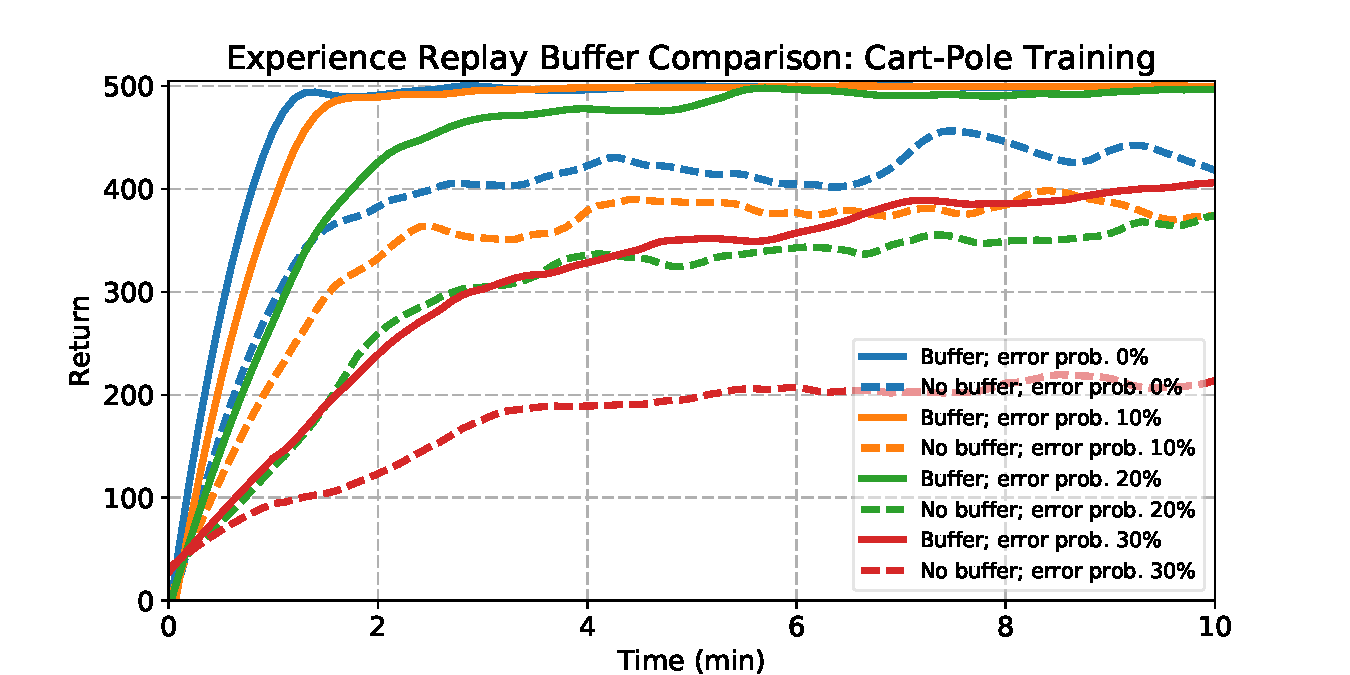
\includegraphics[width=0.9\linewidth]{imagenes/cap3/buffer_cart_pole.pdf}
    \caption{Comparison between using or not experience replay buffer for different values of $P_\mathit{err}$ in the Cart-Pole problem. Buffer: $K = 200$; $b = 10$; $N = 50$. $P_{h}$: $\alpha = 0.6$; $\tau = 0.0003$. Simulated teacher network learning rate: $0.0003$.}
    \label{fig:buffer_cart_pole}
\end{figure}

\begin{figure}[t]
    \centering
    \vspace{-0.2cm}
    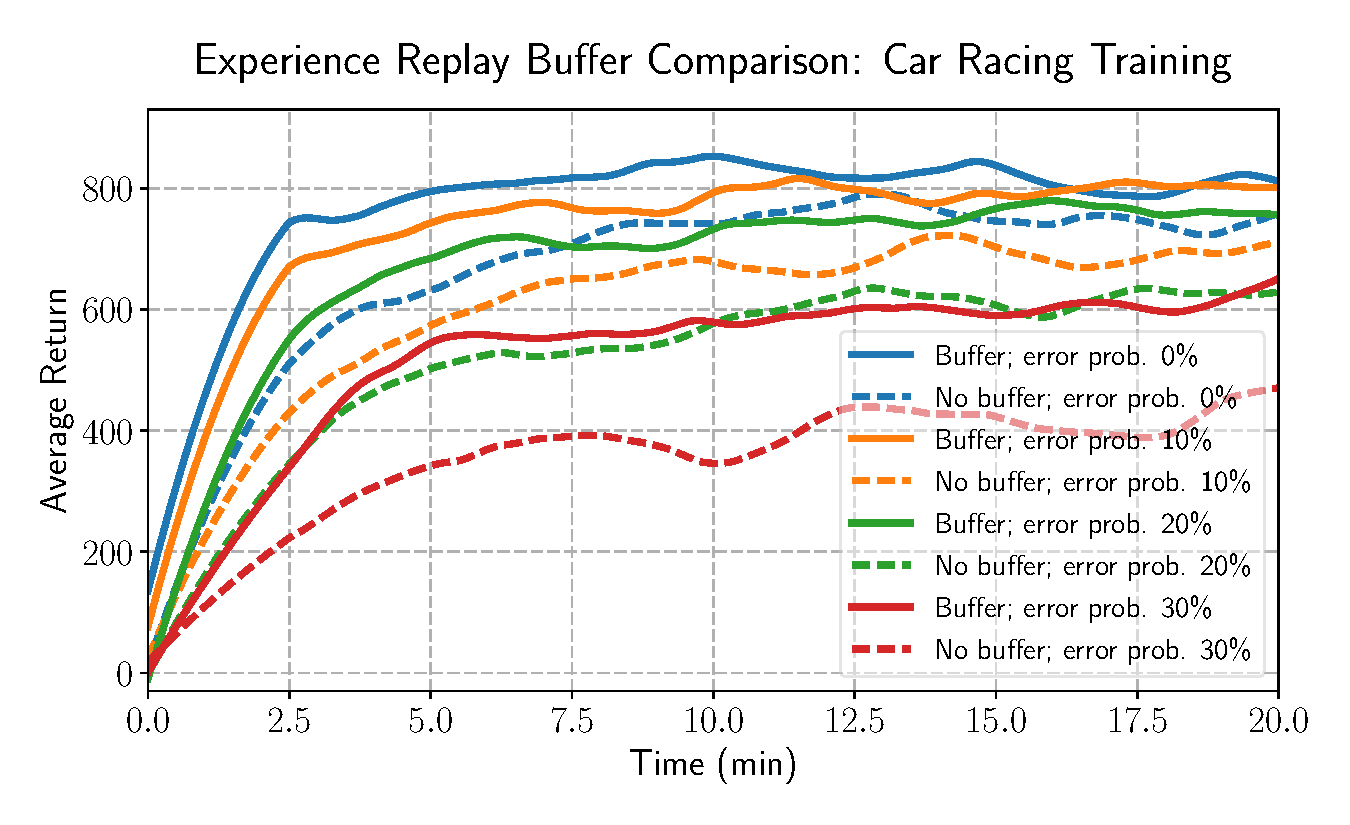
\includegraphics[width=0.9\linewidth]{imagenes/cap3/bufferCarRacing.pdf}
    \vspace{-0.2cm}
    \caption{Comparison between using or not experience replay buffer for different values of $P_\mathit{err}$ in the CarRacing problem. Buffer: $K = 1000$; $b = 10$; $N = 100$. $P_{h}$: $\alpha = 0.6$; $\tau = 0.000015$. Simulated teacher network learning rate: $0.0003$.}
    \label{fig:buffer_car_racing}
\end{figure}

In \figurename~{\ref{fig:buffer_cart_pole}} and \figurename~{\ref{fig:buffer_car_racing}} the learning curves show a large difference between the processes of learning that use experience replay buffer with respect to the cases without the buffer. In the case without the buffer, which is more similar to the original COACH, it is possible to see that the learning agent is not benefiting from the advised corrections as much as it can do when the pieces of advice are kept in the memory. For instance, we can see that $\text{D-COACH}$ v1 learns more from corrections with $20 \%$ of mistakes when using the buffer than in the case of perfect corrections, but without any buffering. This means the buffer is necessary for increasing the use of the available information, even when this information could be corrupted and not clean.

\subsection{Comparison of DRL and D-COACH using real human teachers}
\begin{figure}[t]
    \centering
    \vspace{-0.2cm}
    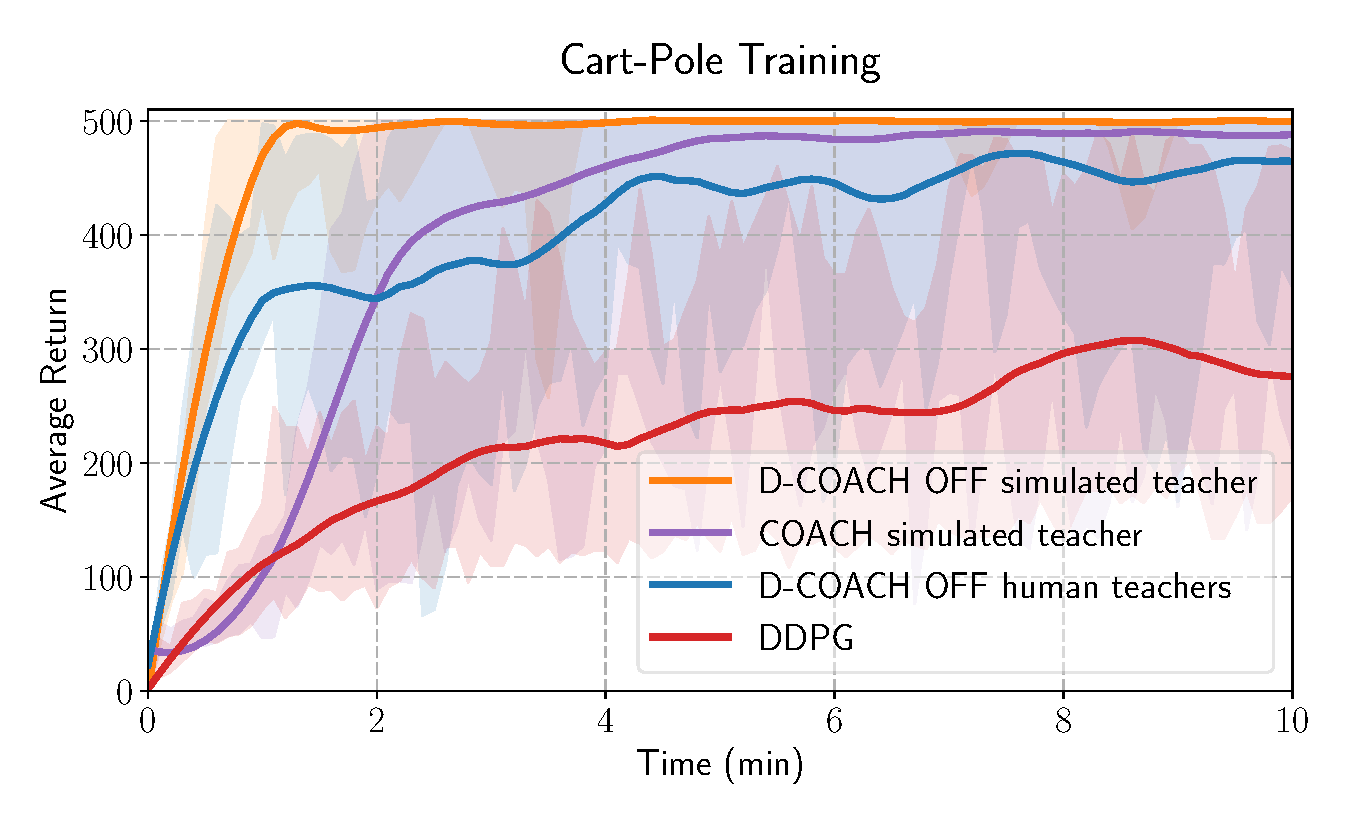
\includegraphics[width=0.9\linewidth]{imagenes/cap3/offline_cart_pole_humans.pdf}
    \vspace{-0.2cm}
    \caption{Cart-Pole training. Buffer: $K = 200$; $b = 10$; $N = 50$. $P_{h}$: $\alpha = 0.6$; $\tau = 0.0003$. Human teacher network learning rate: $0.003$; Simulated teacher network learning rate: $0.0003$.}
    \label{fig:cartpole_results}
\end{figure}

These experiments are intended to compare the learning process of D-COACH (simulated teacher and human teacher) with the DRL algorithm DDPG. Taking into account that the Cart-Pole problem has a low dimensional state space, the original COACH, based on basis functions, is also included in the comparison. In this case, $P_\mathit{err}=0\%$ was used for the simulated teachers. The results of this problem are shown in \figurename~{\ref{fig:cartpole_results}}, wherein it is possible to see that COACH-like methods outperform the DRL agent with a large difference. When using the simulated teacher, D-COACH v1 learns faster than the original COACH. The performance of D-COACH v1 with human teachers decreases with respect to the simulated teacher. This is because human teachers are not perfect and make mistakes, but they are being compared with a simulated teacher with $P_\mathit{err}=0\%$, which means that it makes no mistakes. Also because the simulated teacher model is quite simple to represent the complexity of the human behavior, then, although it is not very realistic, it is still useful for comparisons of interactive learning strategies under similar conditions.

In \figurename~{\ref{fig:racing_car_results1}} the learning curves of the Car Racing problem are presented. Again, D-COACH v1 results in a fast convergence. Unlike reported results of DRL algorithms for this problem, in the very early minutes D-COACH v1 reaches high performance policies that have not been obtained by most of the DRL approaches, to the best of our knowledge. If we compare a policy trained with D-COACH v1 for approximately 75 minutes by an experienced teacher against several state-of-the-art DRL approaches, it can be seen that it outperforms most of them (see Table \ref{CarRacing_table}). The problem is considered to be solved if the agent gets an average score of 900 or more over 100 random tracks. However, we observed that this value can substantially vary between different evaluations, so in Table \ref{CarRacing_table}, the obtained range of values over 20 evaluations is presented for D-COACH v1.
\vspace{-0.4cm}

\begin{figure}[t]
    \centering
    \vspace{-0.2cm}
    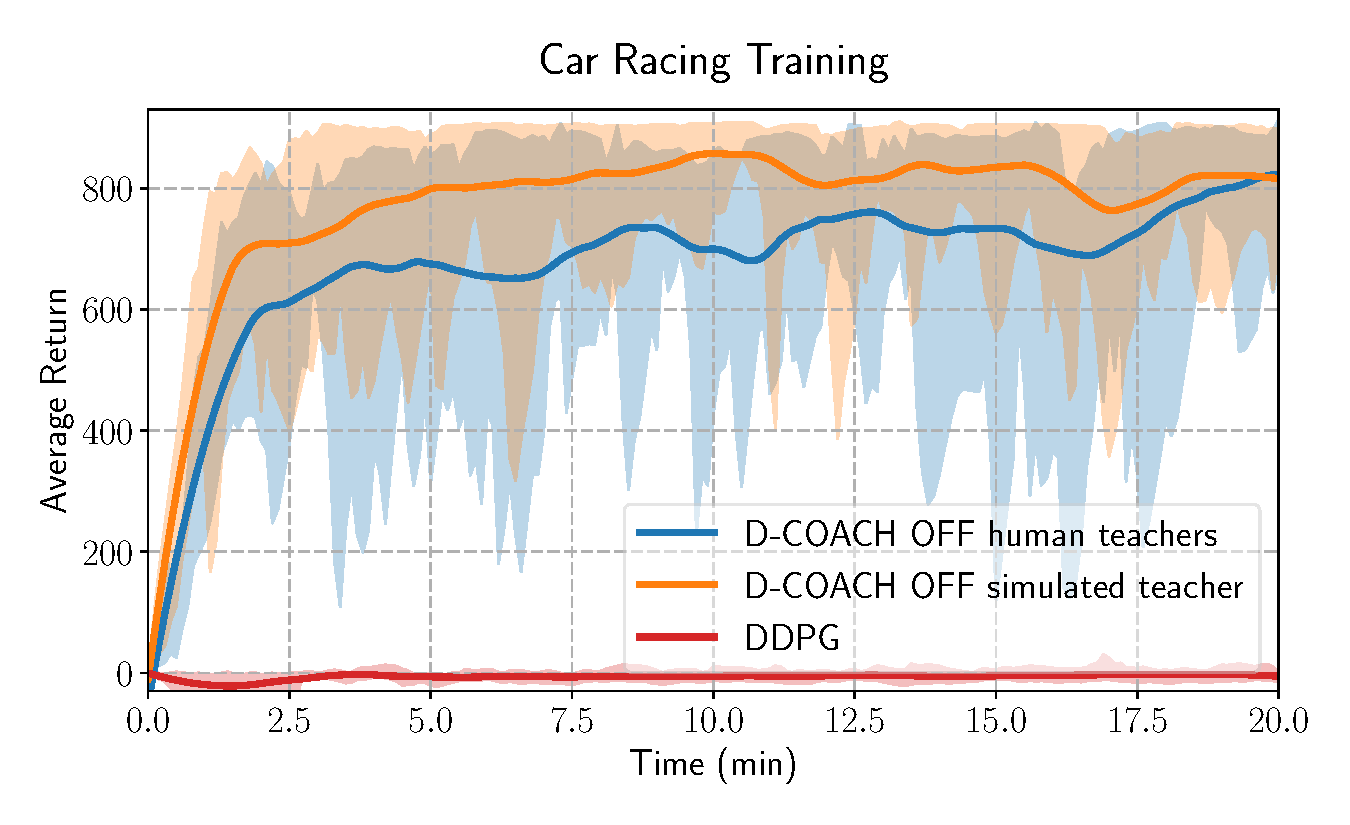
\includegraphics[width=0.9\linewidth]{imagenes/cap3/offline_car_racing_humans.pdf}
    \vspace{-0.2cm}
    \caption{Racing Car training. Buffer: $K = 1000$; $b = 10$; $N = 100$. $P_{h}$: $\alpha = 0.6$; $\tau = 0.000015$. Human teacher network learning rate: $0.001$; Simulated teacher network learning rate: $0.0003$.}
    \label{fig:racing_car_results1}
\end{figure}

\begin{table}[t]
\centering
\caption{Car Racing state-of-the-art learning algorithms comparison. DRL results taken from \cite{Ha2018}.}
\label{CarRacing_table}
\begin{tabular}{lc}
\multicolumn{1}{c}{\textbf{Method}}      & \multicolumn{1}{l}{\textbf{Average Score over 100 Random Tracks}} \\ \hline\hline
DQN                                      & 343 $\pm$ 18                                                      \\ \hline
A3C (continuous)                         & 591 $\pm$ 45                                                      \\ \hline
A3C (discrete)                           & 652 $\pm$ 10                                                      \\ \hline
ceobillionaire’s algorithm (unpublished) & 838 $\pm$ 11                                                      \\ \hline
Full World Model                         & 906 $\pm$ 21                                                      \\ \hline
\textbf{D-COACH (experienced teacher)}                         & \textbf{895 - 909 $\pm$ 18 - 80} \\
& \textbf{Average over 20 evaluations: 903 $\pm$ 46}
\\ \hline
\end{tabular}
\end{table}

\subsection{Validation in a real system}
In the third problem that we called Duckie Racing, an agent has to learn to drive a Duckiebot (from the project  Duckietown \cite{Paull2017} with modifications from the Chile Duckietown Team\footnote{\url{https://github.com/Duckietown-Chile/}}) autonomously through a track based on raw visual information of an onboard camera. The actions in this problem are the forward speed and the steering angle of the Duckiebot. Two tasks are set for this environment: (i) driving the Duckiebot freely through the track, with permission to drive in both lanes, and (ii) driving the Duckiebot only in the right lane, which demands more accuracy in driving. In this problem, an episode stops if the robot leaves the track/right lane, or after 30 seconds. The performance index in this task is the percentage of the total track length traveled during the episode. Hence the faster and more accurate the Duckiebot drives, the more distance it will travel.

This problem is not used for comparisons of the methods, but only as a validation of D-COACH using experience replay, which showed to be the best alternative in the previous problems. \figurename~\ref{fig:racing_duckie_results} shows the learning curve for each of the tasks explored in this environment with a real robot and a real human teacher. The curves and a video\footnote{https://youtu.be/vcEtuRrRIe4} attached to this thesis show that the system quickly learns to drive properly through the road based only on the human corrections. As expected, the policy is faster when the robot has the freedom to drive over both lanes. Learning this task with RL would definitely take more training time, and might need an external perception system to compute the reward function, whereas with D-COACH this performance index does not have any influence on the learning process, rather it is used for descriptive and comparative purposes.

\begin{figure}[H]
    \centering
    \begin{minipage}{.5\textwidth}
    \vspace{-0.2cm}
    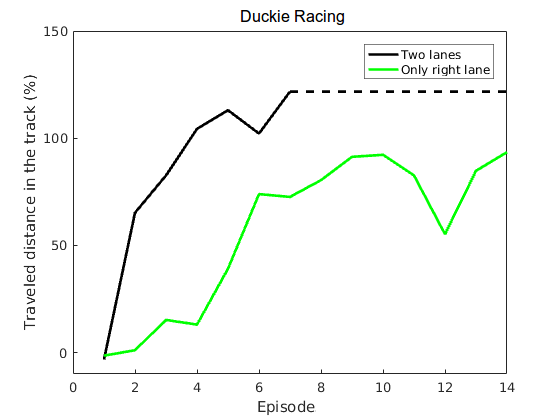
\includegraphics[width=1.0\linewidth]{imagenes/cap3/racing_duckie_results.png}
    \vspace{-0.2cm}
    \caption{Duckie Racing training.}
    \label{fig:racing_duckie_results}
    \end{minipage}%
    \begin{minipage}{.5\textwidth}
    \centering
    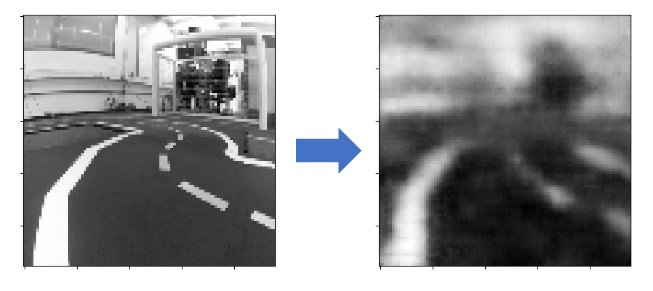
\includegraphics[width=1.0\linewidth]{imagenes/cap3/AE_duckie2.png}
    \vspace{-0.2cm}
    \caption{Duckie Racing autoencoder input (left) vs output (right).}
    \label{fig:AE_duckie}
    \end{minipage}
\end{figure}

\section{Discussion}
This chapter presented D-COACH v1, an algorithm for training policies modeled with DNNs interactively with corrective advice. The method was validated in a problem of low-dimensionality, along with problems of high-dimensional state spaces like raw pixel observations, with a simulated and a real robot environment, and also using both simulated and real human teachers. 

The use of the experience replay buffer (which has been well tested for DRL) was re-validated for this different kind of learning approach, since this is a feature not included in the original COACH. The comparisons showed that the use of memory resulted in an important boost in the learning speed of the agents, which were able to converge with less feedback, and to perform better even in cases with a significant amount of erroneous signals.  

The results of the experiments show that teachers advising corrections can train policies in fewer time steps than a DRL method like DDPG. So it was possible to train real robot tasks based on human corrections during the task execution, in an environment with a raw pixel level state space. 

The comparison of D-COACH with respect to DDPG, shows how this interactive method makes it more feasible to learn policies represented with DNNs, within the constraints of physical systems. DDPG needs to accumulate millions of time steps of experience in order to obtain good performances as shown in \cite{Lillicrap2015}. However, this is not always possible with real systems.
\chapter{Enhancing D-COACH for High-Dimensional State Problems}
\section{Overview}

In this chapter we introduce  D-COACH v2, a variation of D-COACH v1 for problems with high-dimensional state spaces. This is motivated by the limitation that D-COACH v1 presents when learning state representations. Recording a database with observations of the environment and training an autoencoder in an offline step can be time consuming and not robust to changes in the environment. Thus, it would be desirable to have a version of D-COACH that eliminates this offline step, learning everything in a single interaction step, as the original COACH does. Hence, an algorithm capable of training all the parameters of the network interactively from scratch. 

\section{Online State Representation Learning}
In order to obtain an algorithm capable of learning interactively from scratch we need to make the networks to converge faster. In the former chapter, an autoencoder was used to learn a low-dimensional representation of high-dimensional states in an offline learning process. In this chapter, we propose to use the autoencoder learning criteria during the interactive learning process, such that both networks (the policy and the autoencoder) share the convolutional layers of the encoder, as shown in Fig.~\ref{fig:msim}.

\begin{figure}[H]
    \centering
    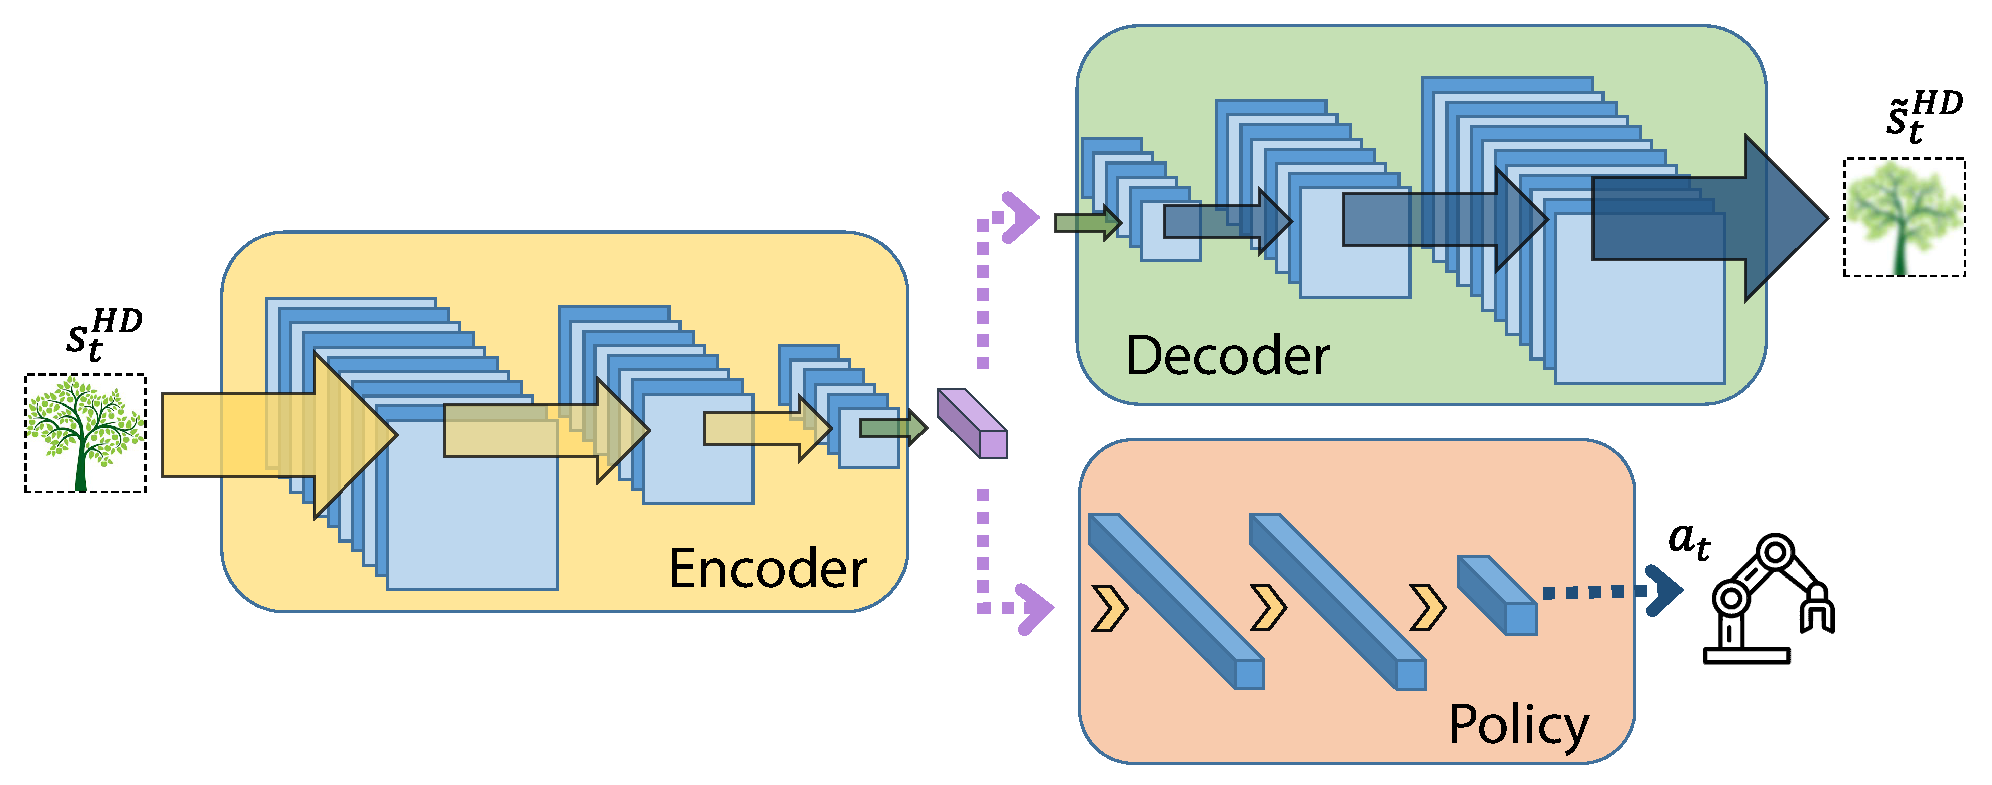
\includegraphics[width=0.6\linewidth]{imagenes/cap2/m2.pdf}
    \caption{D-COACH online state learning. The state representation is shared between the autoencoder and the policy training.}
    \label{fig:msim}
\end{figure}

The policy network has the convolutional layers at the input, followed by a second part that is a fully-connected layer, then this network maps STATE into ACTION, while the autoencoder network involves the computation from STATE to STATE$^{*}$, wherein  STATE$^{*}$ is the reconstructed image at the output of the decoder. Autoencoding is seen as an additional auxiliary criteria for training the state representation of the policy online. 

%So, in addition to the loss function for predicting the policy based on the data generated by the human corrections, it also includes the loss function of the reconstruction at the output of the autoencoder, based on the same data stored during the human corrections. 

\section{The Algorithm}
Algorithm \ref{algorithm:EnDeepCOACH} describes D-COACH ON. The algorithm first sets the hyper-parameters like the magnitude of the error (Equation \ref{eq:error}), and the ones used for the corrections replay. In cases when the teacher advises a correction (line 15), the subsequent lines are evaluated, wherein the policy network is updated along with the autoencoder network.

Two different updates are computed, one for the layers involved in the policy computation, and another for the layers of the autoencoder. When feedback is given by the teacher, the \textbf{update} \emph{policy} instruction updates the policy network for the current time step only using this last received feedback. Subsequently, the \emph{batch\_update} subroutine is called. This subroutine is in charge of updating the policy and the autoencoder by sampling a mini-batch from the replay buffer. The \emph{batch\_update} subroutine is also called every $b$ time steps (line 24).

When the \emph{batch\_update} subroutine is called, the autoencoder is updated only if its reconstruction error in the last \emph{m} observations (MSE between STATE and STATE$^{*}$) is greater than a threshold $\epsilon$ (line 6). Otherwise, the autoencoder is not updated and the convolutional layers of the encoder are frozen. As a consequence, the instruction \textbf{update} \emph{policy} in lines 5 and 19 only modifies the non-convolutional layers of the policy. 

The condition for training the autoncoder is used for avoiding conflicts in the gradients of both cost functions, so when the latent vector of the autoencoder is considered a good smaller representation of the state, the gradient of the policy must be prevented from harming the learned encoding. Hence, the encoder is kept frozen, unless unknown regions of the state space are visited. 

\begin{algorithm}[h]
\caption{D-COACH v2: Online State Representation Learning learning}\label{algorithm:EnDeepCOACH}
\begin{algorithmic}[1]
\algdef{SE}[SUBALG]{Indent}{EndIndent}{}{\algorithmicend\ }%
\algtext*{Indent}
\algtext*{EndIndent}

\State \textbf{Require:} error magnitude $\textit{e}$, buffer update interval $b$, buffer sampling size $N$, buffer max. size $K$, buffer min. size $k$, sequence length for AE reconstruction error \emph{m}, pre-trained encoder parameters (if 3-step sequential learning) 
\State \textbf{Init:} $B = []$ \emph{\# initialize memory buffer}

\colorbox{lightgray}
{\parbox{\linewidth}{\State \textbf{function} batch\_update \emph{\# define batch update function}
\Indent
\If{$\mathrm{length}(\mathcal{B}) \geq k$}
\State \textbf{update} \emph{policy} using SGD with a mini-batch sampled from $B$
\If{$AE_{\mathrm{error}}>\epsilon$}
\State \textbf{unfreeze} convolutional layers
\State \textbf{update} $AE$ using SGD with a mini-batch sampled from $B$
\Else
\State \textbf{freeze} convolutional layers
\EndIndent
\EndIf
\EndIf
}}
\colorbox{lightlightgray}{\parbox{\linewidth}{%
\For{t = 1,2,...}{} \emph{\# main loop}
\State \textbf{observe} state $s_{t}$
\State \textbf{execute} action $a_{t}=\pi(s_{t})$
\State \textbf{feedback} human corrective advice $h_{t}$
\If{$h_{t}$ is not \textbf{0}}
\State $\mathrm{error}_{t} = h_{t}\cdot e$
\State $y_{\mathrm{label}(t)} = a_{t} + \mathrm{error}_{t}$ 
\State \textbf{update} \emph{policy} using SGD with pair ($s_{t}$, $y_{\mathrm{label}(t)}$) 
\State \textbf{call} batch\_update
\State \textbf{append} $(s_{t}, y_{\mathrm{label}(t)})$ to $\mathcal{B}$
\EndIf
\If{length($B$) $> K$ }
\State $\mathcal{B} = \mathcal{B}[2:K+1]$
\EndIf
\If{$\operatorname{mod}(t, b)$ is 0}
\State \textbf{call} batch\_update
\EndIf
\EndFor}}
\end{algorithmic}
\end{algorithm}

\section{Experiments and Results}

Three different types of experiments were carried out for validating this version of D-COACH: i) experiments with simulated teachers for evaluating the learning method under controlled conditions without influence of human factors, ii) validations with real human teachers, and iii) extra validations on real physical systems.

%In these experiments we denote the enhanced D-COACH simply with `D-COACH', while from now on we call the previous version `basic D-COACH'. 

In the experiments, the learning processes are analyzed in three different problems:

\textbf{(i) Car Racing:} Exactly the same problem as the one used in Chapter 2. The coupled feedback strategy was also used in this case. 
    
\textbf{(ii) Duckie Racing:} Also the same problem as the one used in Chapter 2 with the difference that now also a simulation of this environment was used \cite{gym_duckietown}. The same map was used for both the simulated and real robot. In the simulations, at the beginning of each episode, the robot can start, randomly, at the points A or B (plus random noise) of the map (see Fig.~\ref{fig:duckietown2}). Each simulated episode lasts 1,000 time steps (unless the robot leaves the road before), and as a performance metric a modified version of the default reward function of the environment is used, which is: $R = Cv\theta - Dd$. $C$ and $D$ are constants ($C=100$, $D=1$), $v$ is speed of the duckiebot, $\theta$ is its orientation with respect to $\gamma$ (a bezier curve that defines the path the agent is expected to follow), and \emph{d} is its distance to $\gamma$.

\begin{figure}[h]
\centering
\subfloat[][Duckiebot.]{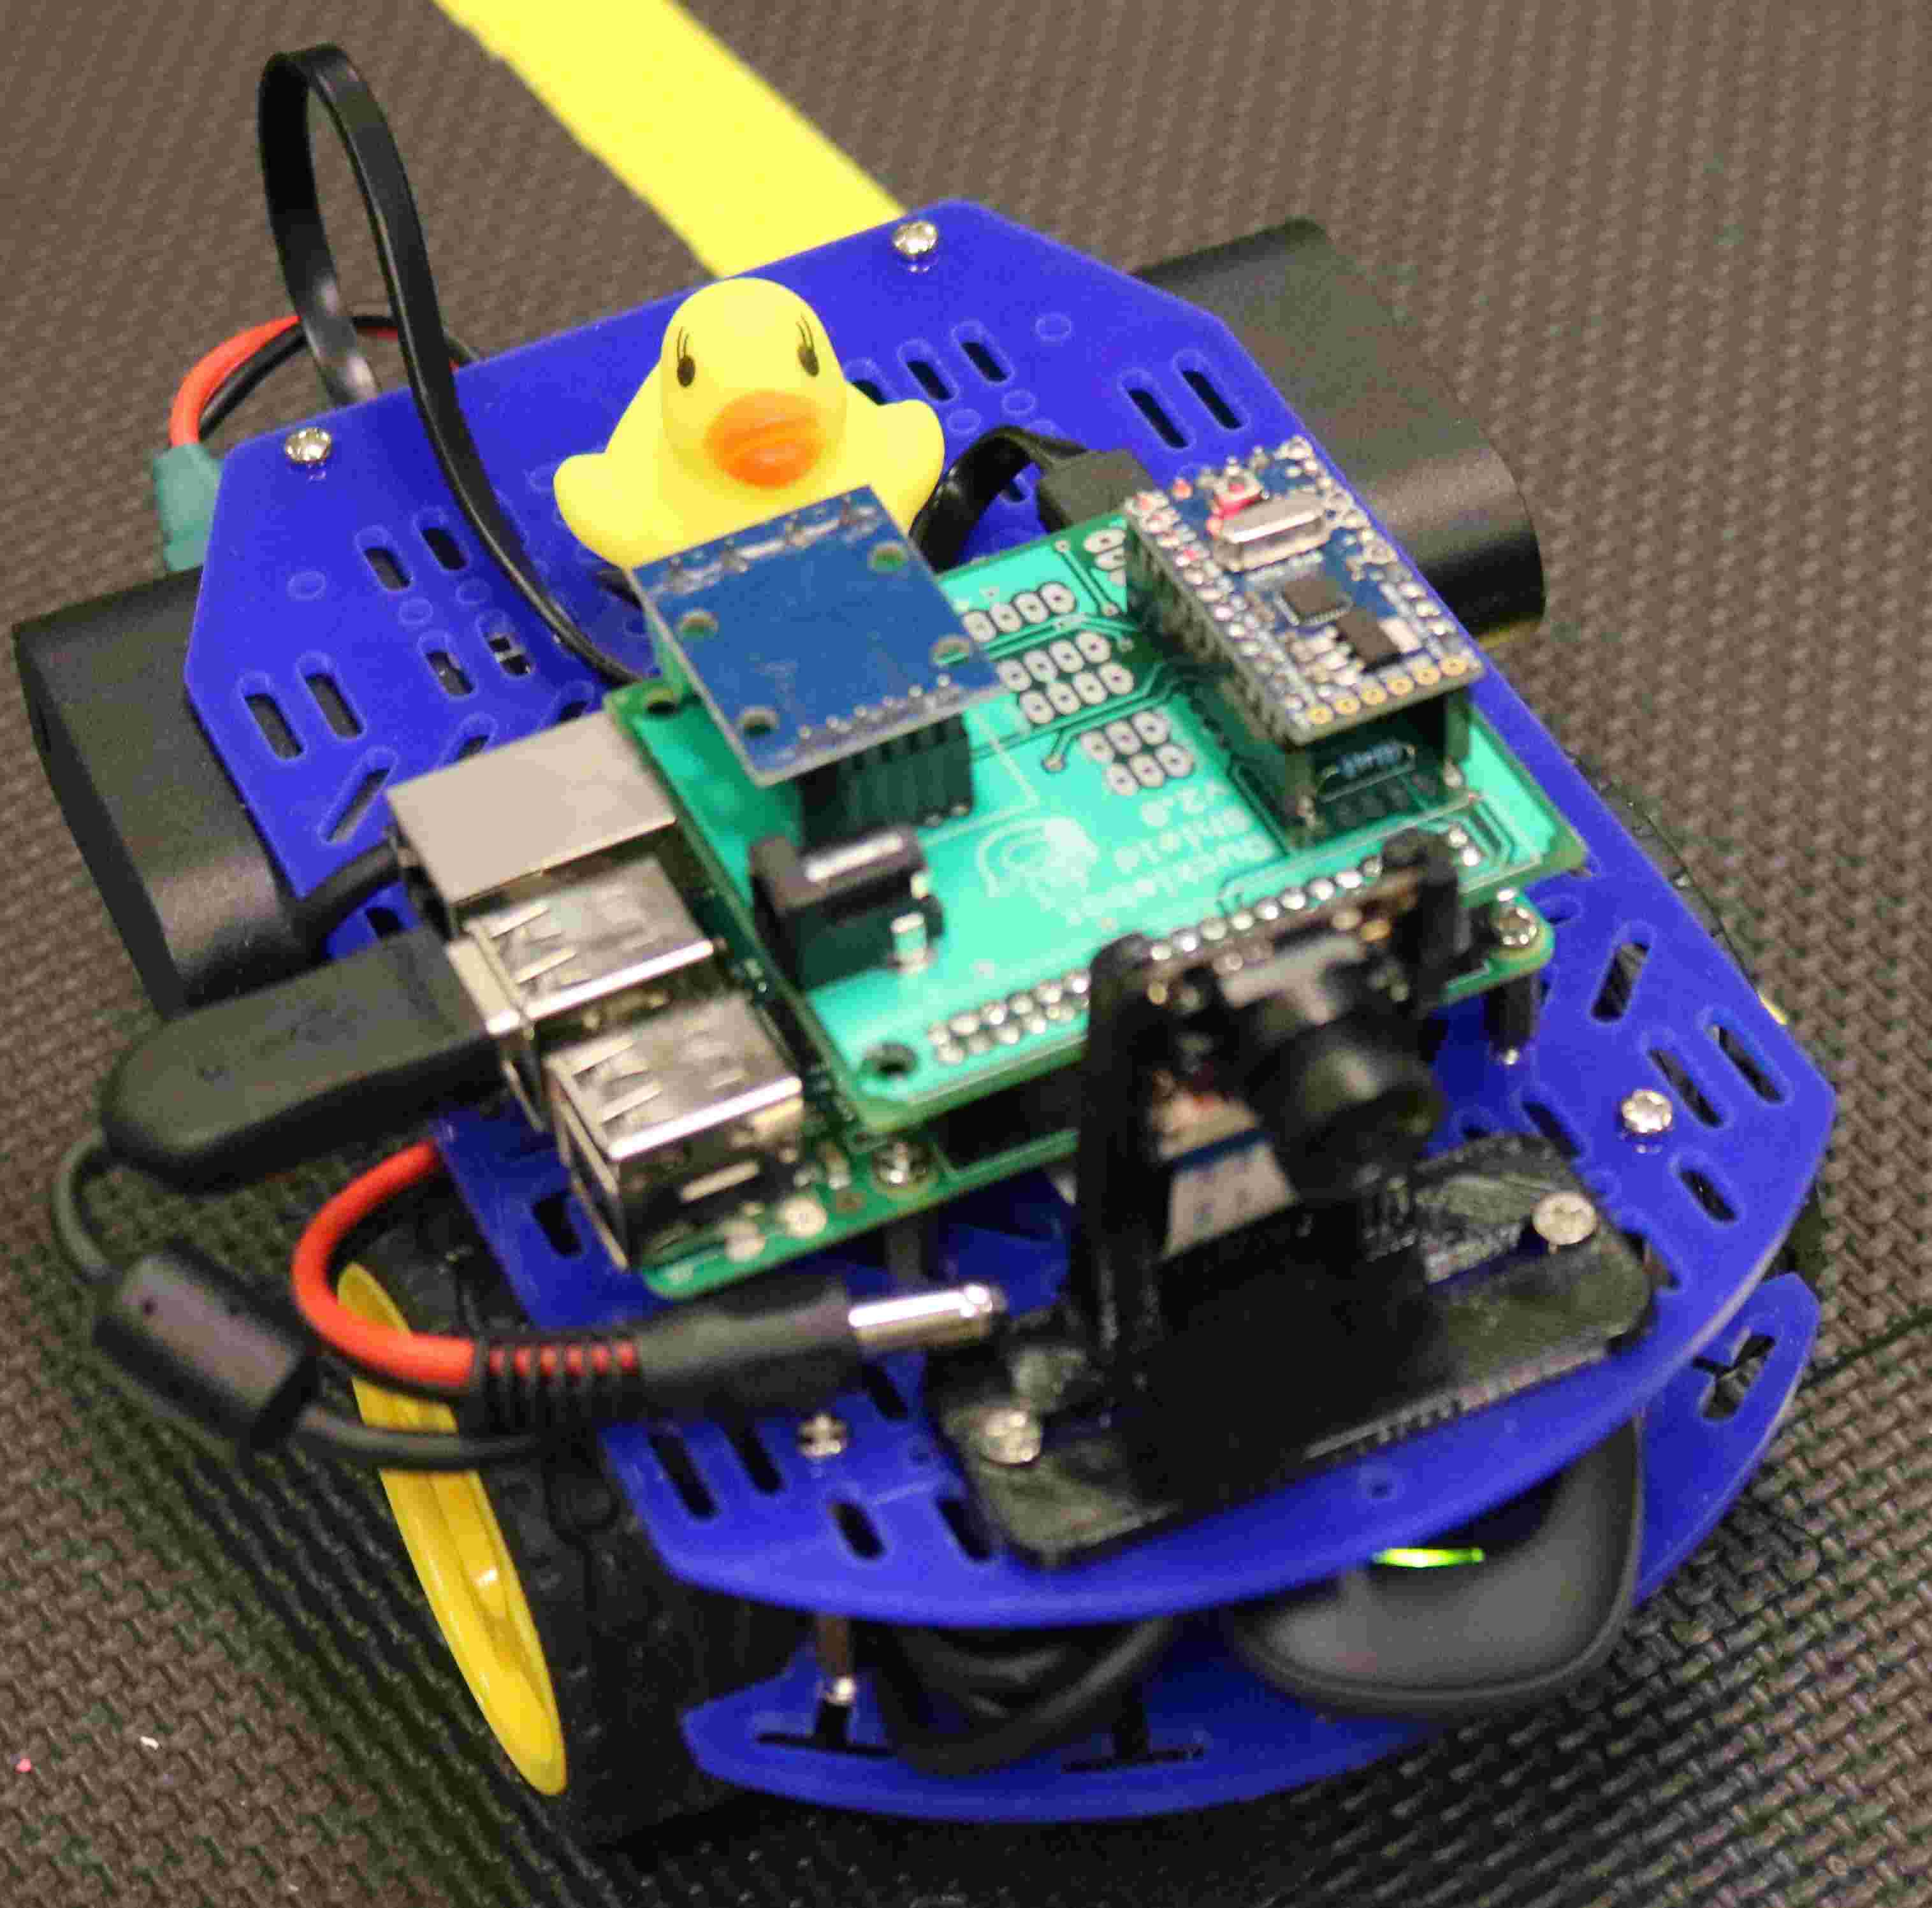
\includegraphics[width=0.305\linewidth]{imagenes/cap3/duckie_image.jpg}} 
\hspace{1.3cm}
\subfloat[][First-person view.]{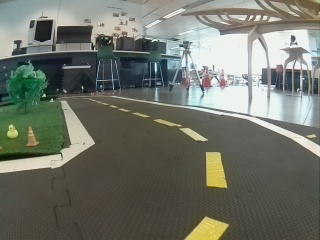
\includegraphics[width=0.4\linewidth]{imagenes/cap3/real_duckie_view.jpg}}
\hspace{2cm}
\subfloat[][Map.]{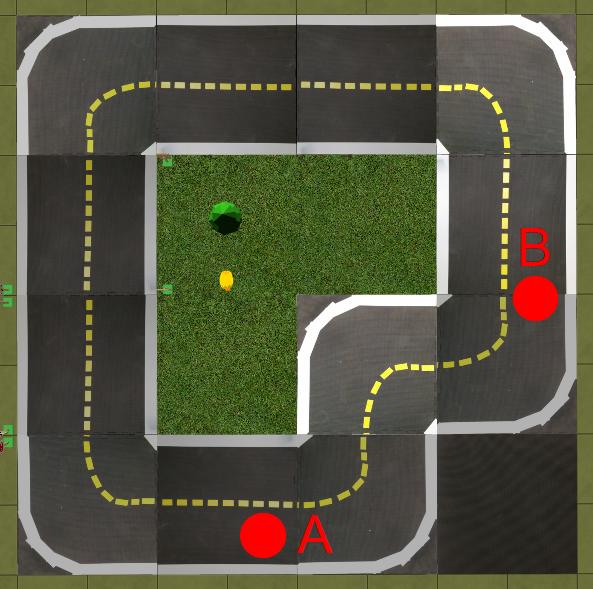
\includegraphics[width=0.305\linewidth]{imagenes/cap3/duckie_map.png}}
\hspace{1.3cm}
\subfloat[][First-person simulated view.]{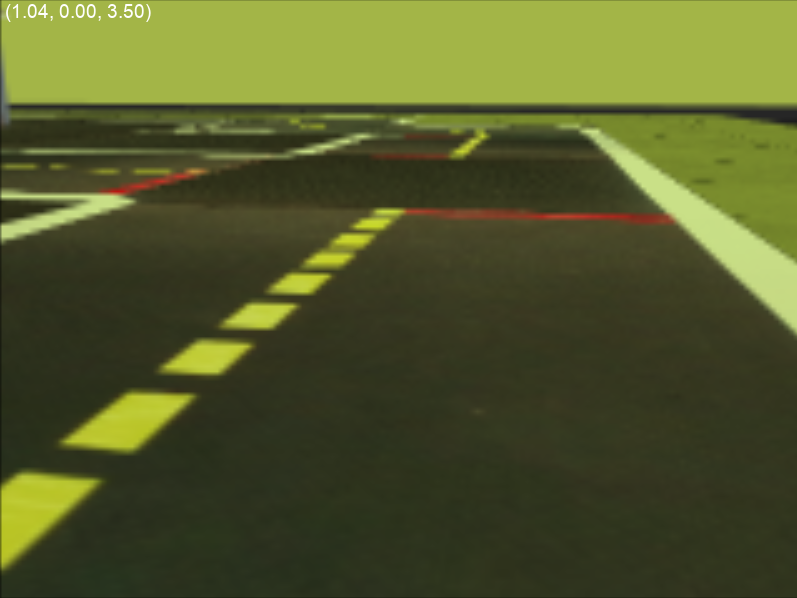
\includegraphics[width=0.4\linewidth]{imagenes/cap3/simplesim_1.png}}
\caption{Duckietown.} 
\label{fig:duckietown2} 
\end{figure}

\textbf{(iii) Pusher/Reacher:} Two validation tasks with a 3DoF robotic arm (see Fig.~\ref{fig:PusherReacher}). The problems of pushing  and reaching an object were addressed.  
For both tasks the robot arm is placed in front of the work-space and an RGB camera is fixed overhead for capturing the top-down view of the environment with images of $640\times480\times3$ size. The images are downsampled to $64\times64\times3$. The objective of the Pusher task is to move the object placed in the work-space down, until it is out, as depicted in Fig.~\ref{fig:PusherReacher}(b). The objective of the Reacher is to track the position of the object with the arm's end effector (Fig.~\ref{fig:PusherReacher}(c)). In these problems, the teacher advises corrections of the position commands of the arm in the Cartesian space. The experiments of the tasks with the 3DoF robot arm were intended only to validate the proposed learning method in another real setup, no comparisons were carried out. These experiments were done at TU Delft by Carlos Celemin, as a part of the paper \emph{"Continuous Control for High-Dimensional State Spaces: An Interactive Learning Approach"}, which is mentioned in the Appendix.

All the results that present averaged data in the form of a curve have confidence intervals that represent the $60^{th}$ percentile of the data.
The neural network hyperparameters proposed in Chapter 3 were used in this work. The experiments are illustrated in the following video \url{https://youtu.be/i4f1D4CH26E}. 

\begin{figure}[h]
\centering
\subfloat[][3DoF robot arm.]{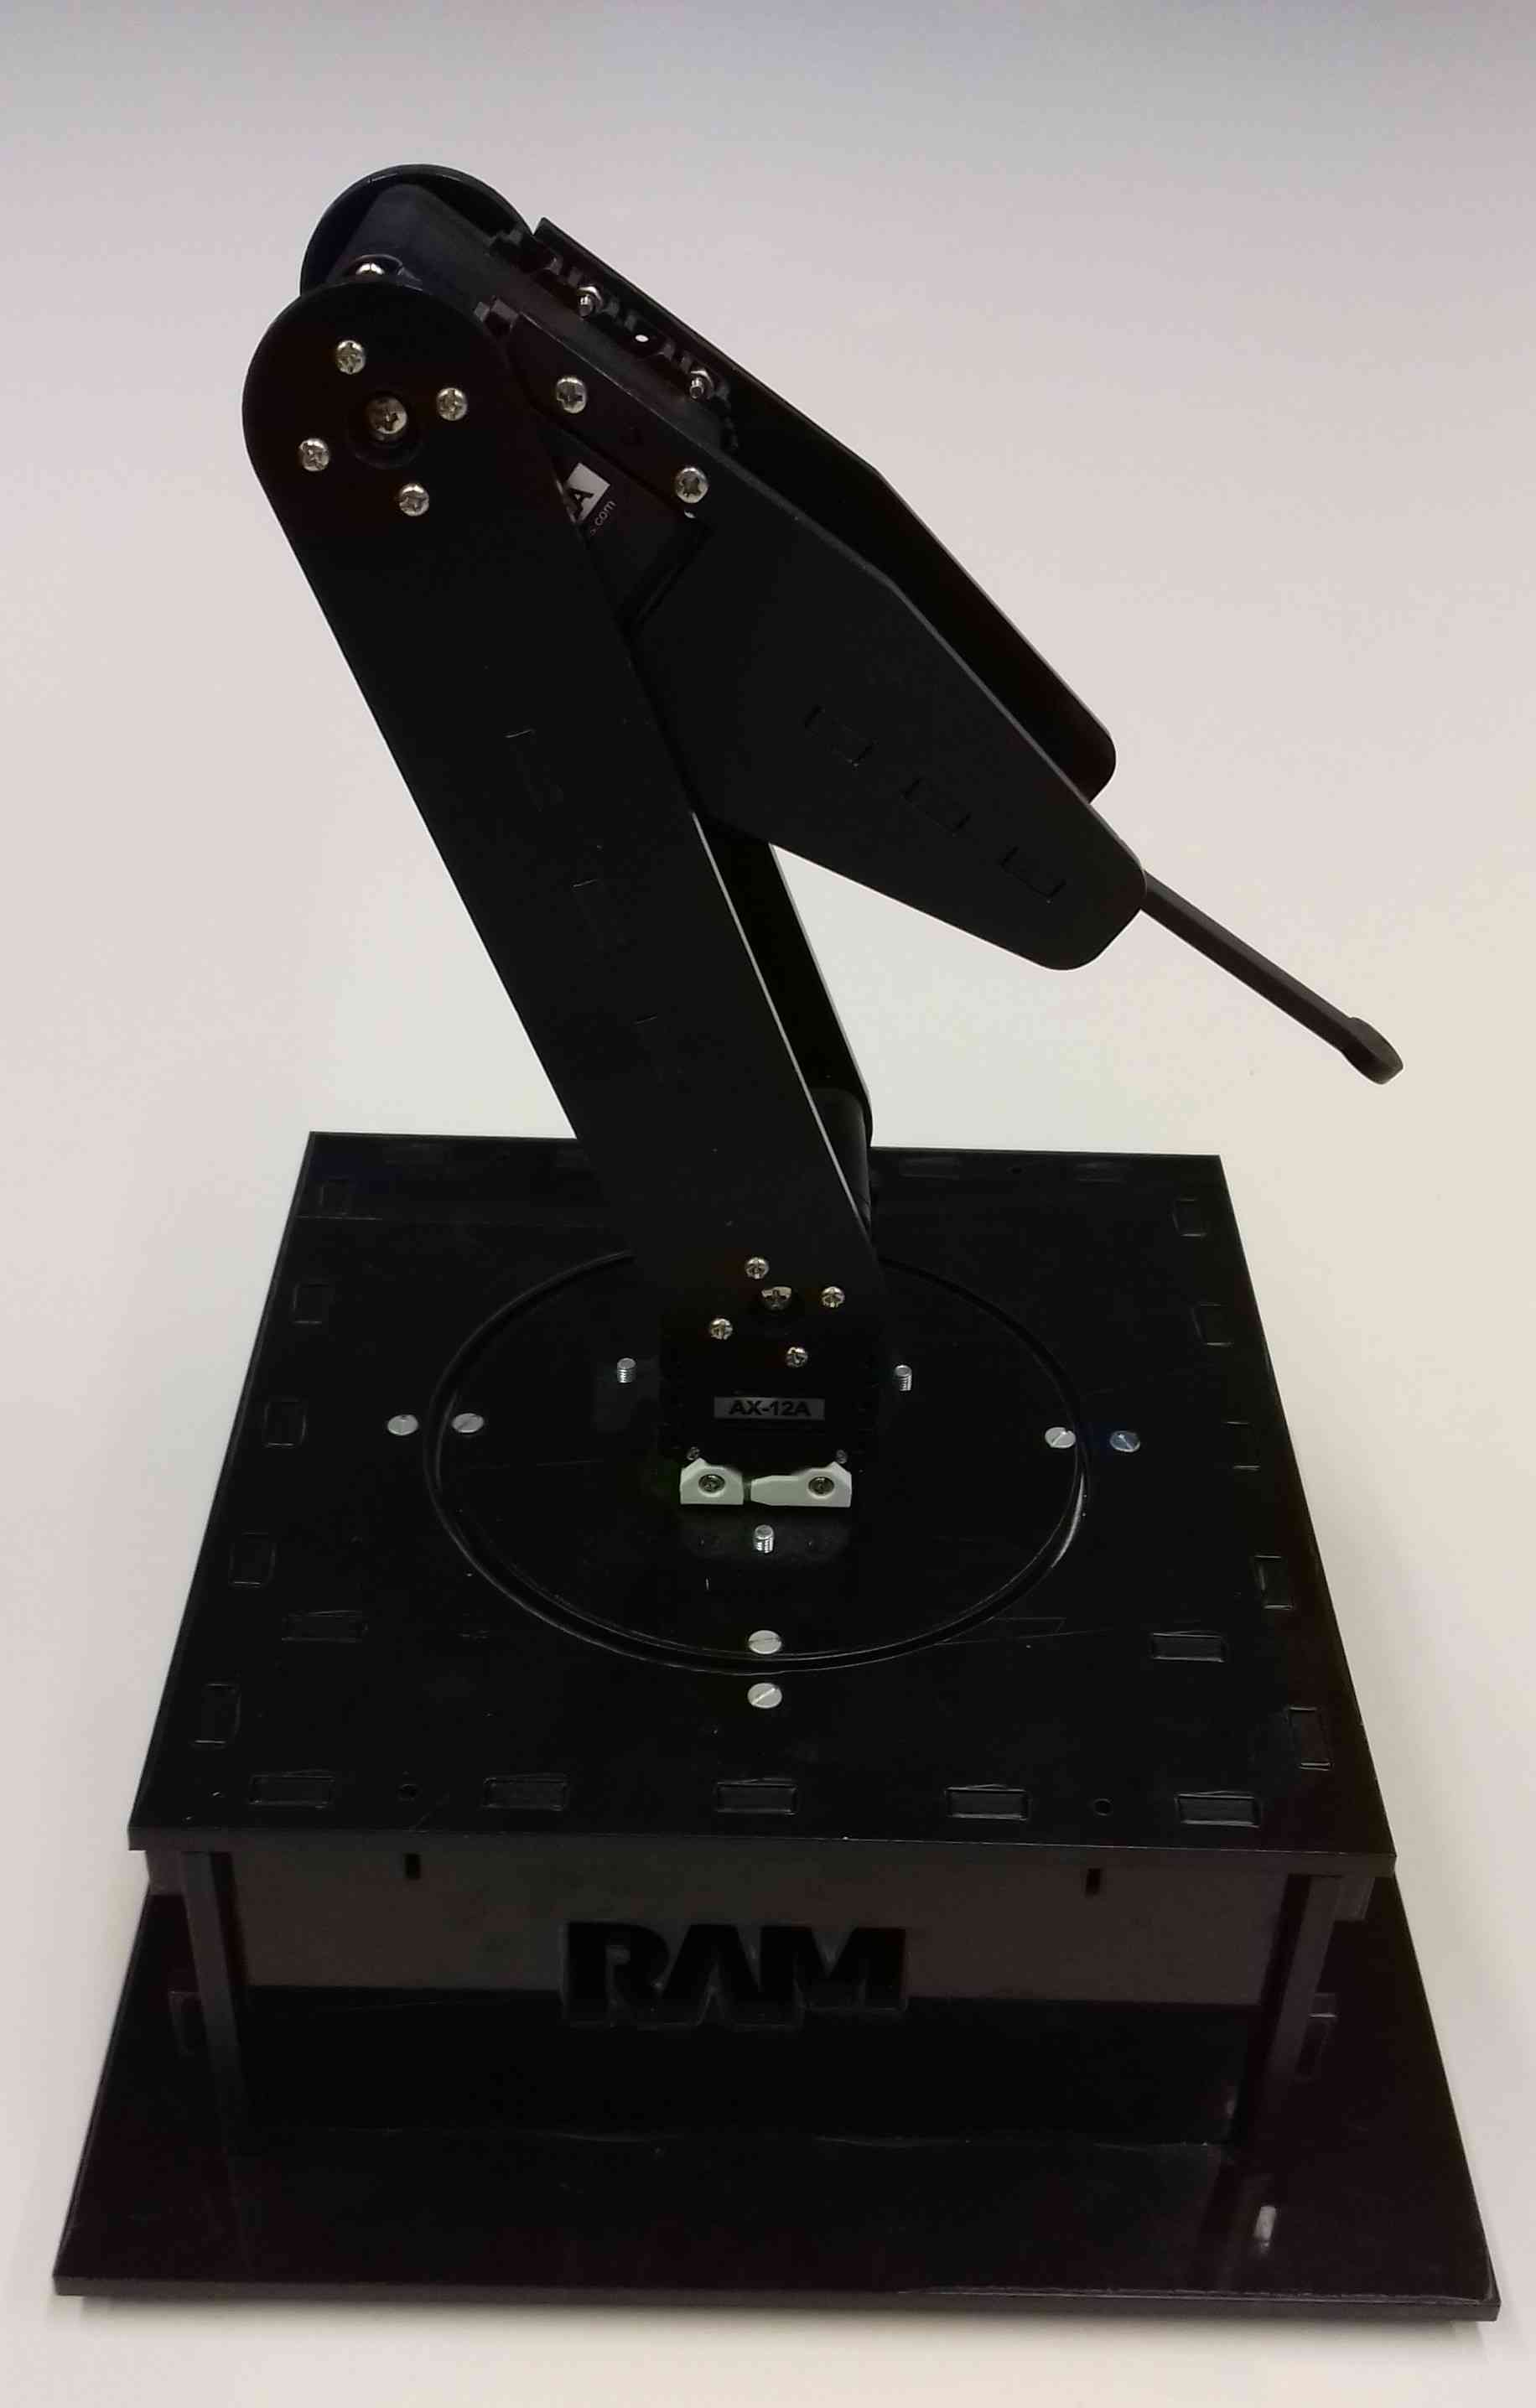
\includegraphics[width=0.2\linewidth]{imagenes/cap3/3dofarm2.jpg}} 
\hspace{0.25cm}
\subfloat[][Pusher task.]{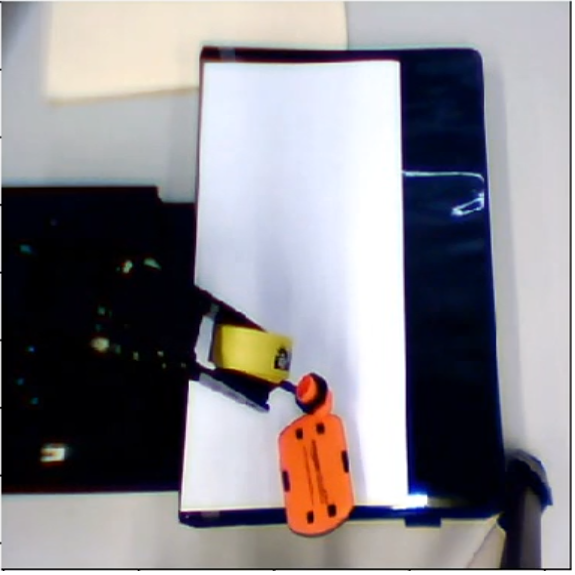
\includegraphics[width=0.315\linewidth]{imagenes/cap3/pusher.png}} 
\hspace{0.25cm}
\subfloat[][Reacher task.]{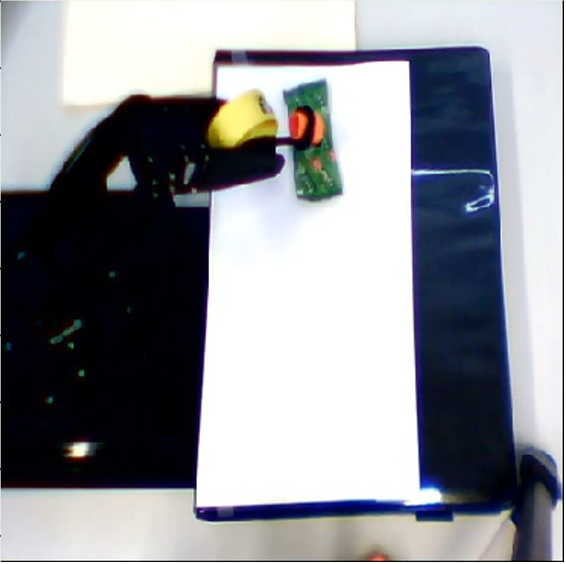
\includegraphics[width=0.315\linewidth]{imagenes/cap3/reacher.png}}
\hspace{0.25cm}
\caption{Pusher/Reacher.} 
\label{fig:PusherReacher} 
\end{figure}


\subsection{Study with Simulated teacher}
In order to evaluate the method along with subtle variants under more controlled conditions, a high performance policy standing-in as a teacher, which was actually trained with $\text{D-COACH}$ v2 and a real human teacher, was used (in the same way as in Chapter 2).

To perform an ablation study that evaluates the contribution of the new components of D-COACH v2, the complete method (Algorithm \ref{algorithm:EnDeepCOACH}) is compared to a second variant that does not include the AE contribution, and learns the whole policy network only with the cost of predicting the action. This variant  works like the D-COACH v1, but skipping the first two steps of recording demonstrations and pre-training the AE, i.e., learning from scratch, which means that the convolutional layers are also learned with the teacher's corrections.

The third evaluated variant includes the AE cost function, but never freezes the convolutional layers, so it always modifies the parameters of the complete policy network using the gradient of both cost functions (i.e. setting $\epsilon=0$ for the condition in line 6). The learning curves of the three cases of D-COACH are compared against a DDPG-based RL agent \cite{Lillicrap2015} implemented by OpenAI \cite{baselines}. The curves are the average of 30 runs for each case, showing the evolution of the return through the learning time. The time considered is measured when rendering the environments, i.e., no environment acceleration, since D-COACH is intended for learning with real systems wherein speeding up the environment is not possible.

As shown in the Fig.~\ref{fig:simulatedteachers} for the experiments with the Car Racing, the complete D-COACH v2 has a considerable improvement when simultaneously using the gradients of the auto-encoding cost function for learning the state representation, along with the gradient of the policy  (blue and orange curves), in contrast to using only the gradient of the policy (green curve), which is slower, and reaches less than $50\%$ of outcome with respect to the complete algorithm after 20 minutes of training. Additionally, there is no noticeable improvement in the performance for the RL agent within this time frame.

\begin{figure}[h]
    \centering
    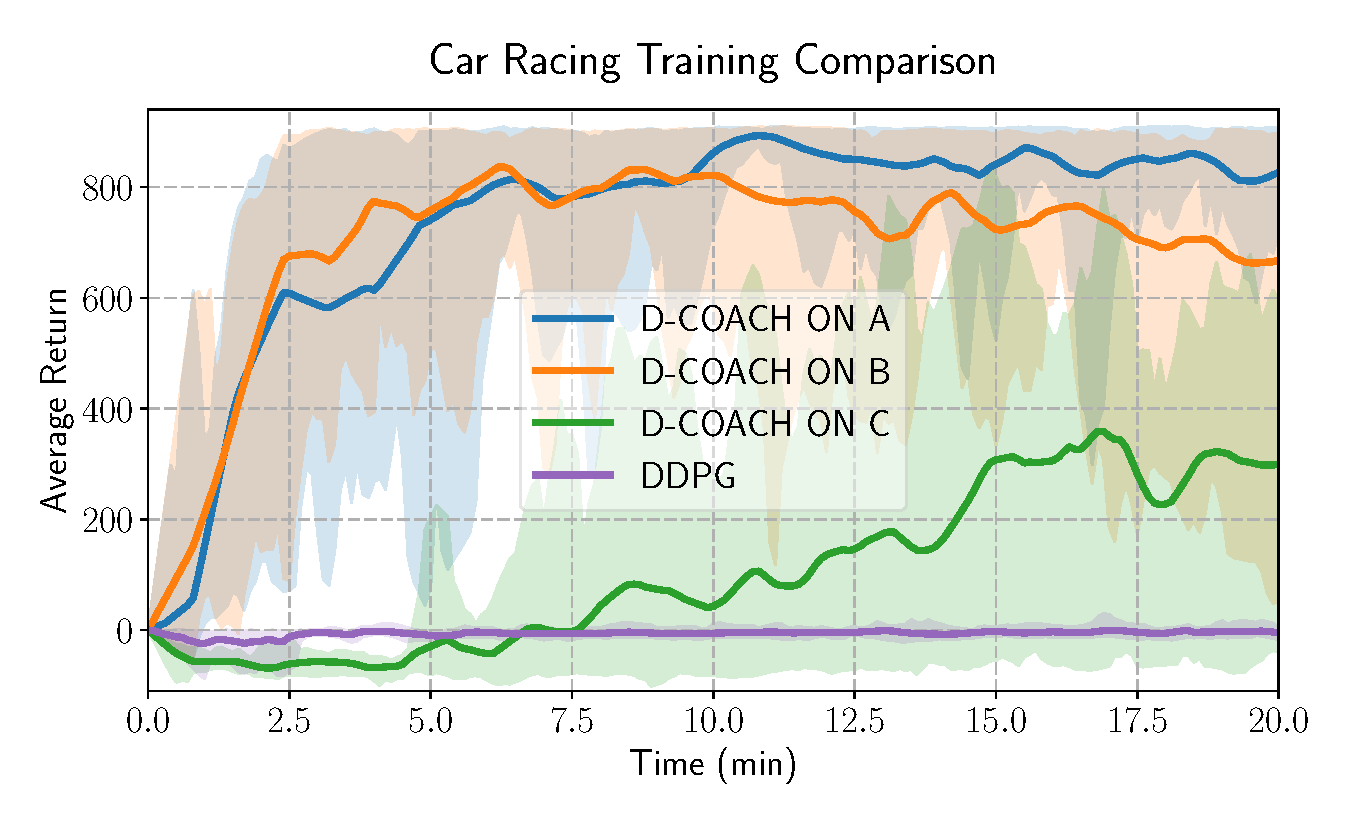
\includegraphics[width=0.9\linewidth]{imagenes/cap3/car_racing_sim_ICRA.pdf}
    \caption{Car Racing results for simulated teacher with D-COACH and DDPG. D-COACH A: policy and AE costs, freezing conv. layers; D-COACH B: policy and AE costs; D-COACH C: only policy cost. Buffer: $K = 1000$; $b = 10$; $N = 8$. $P_{h}$: $\alpha = 0.6$; $\tau = 0.000015$.}
    \label{fig:simulatedteachers}
\end{figure}

\begin{figure}[h]
    \centering
    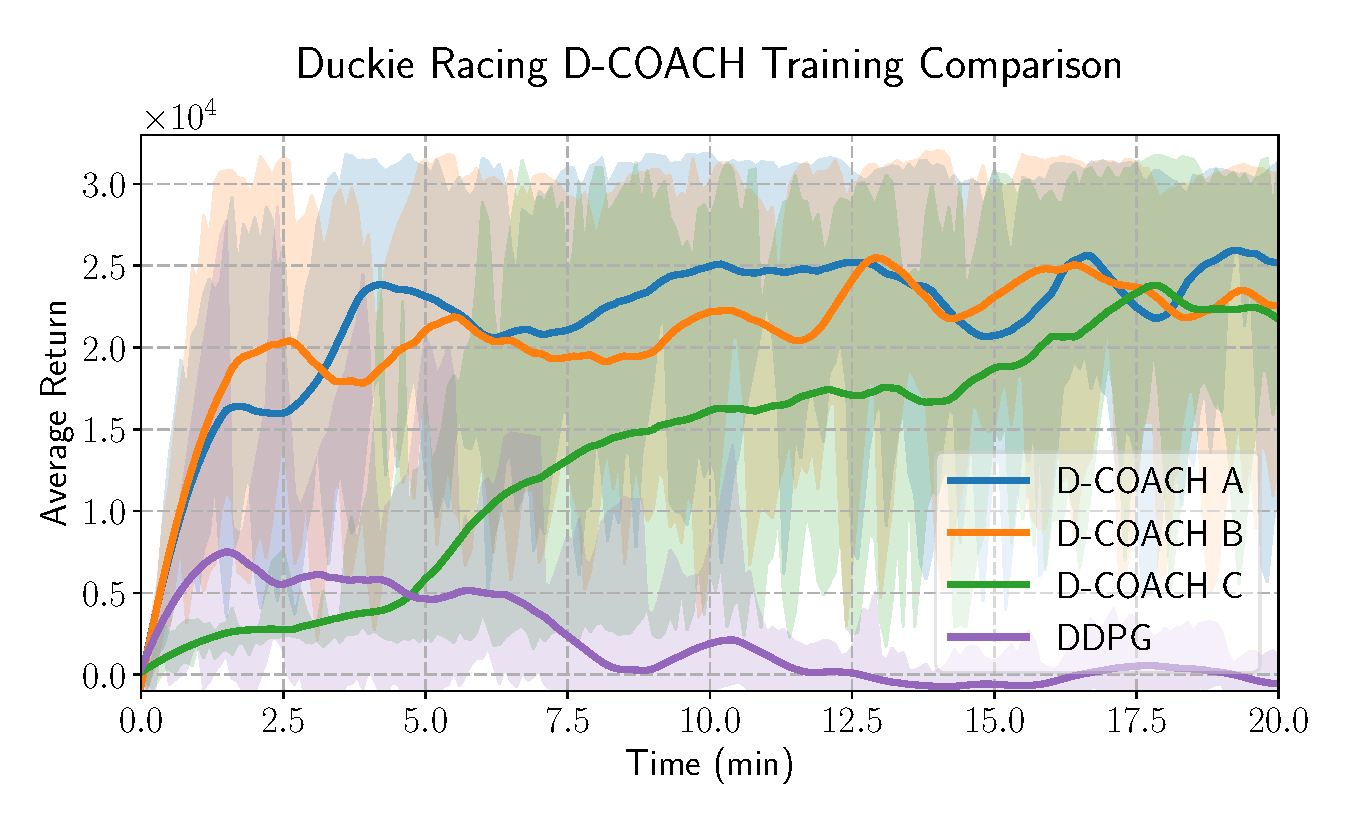
\includegraphics[width=0.9\linewidth]{imagenes/cap3/duckie_sim_ICRA.pdf}
    \caption{Duckie Racing results for simulated teacher with D-COACH and DDPG. D-COACH A: policy and AE costs, freezing conv. layers; D-COACH B: policy and AE costs; D-COACH C: only policy cost. Buffer: $K = 1000$; $b = 10$; $N = 8$. $P_{h}$: $\alpha = 0.6$; $\tau = 0.000015$.}
    \label{fig:racing_car_results}
\end{figure}

The results of the experiments with the Duckie Racing problem (Fig.~\ref{fig:simulatedteachers}) show similar trends as observed with the Car Racing problem, wherein the contribution of the AE cost function makes a considerable difference with respect to only using the policy cost. However, in this problem the variant of D-COACH using only the policy cost manages to reach the same level of performance of the other variants after 17 minutes of training. This variant can learn good policies for this problem, but for reaching $95\%$ of the final performance, it is around 5 times slower than the variants using simultaneous auto-encoding. For this problem again the DDPG learning process does not obtain any improvement during the first 20 minutes of the learning process. 

Finally, it is possible to see the contribution of the condition stated for freezing the convolutional layers, when the error of the decoder is small. This rule provides more stability to the learning process. In the Car Racing experiments, the variant that always updates the AE undergoes an ``unlearning'' stage after 10 minutes of training, whereas in the Duckie Racing experiments is not possible to notice any considerable difference between both approaches. When the error of the decoder is small it means that the latent vector is a good representation of the state, but still the gradient and the error of the policy can be large; therefore, in some cases there may be conflicts that harm the AE performance and consequently the performance of the policy. Freezing these layers is a detail that solves this conflict.

\subsection{Experiments with real human teachers}

The experiments with simulated teachers are useful for analyzing the evolution of the learning process. However, D\nobreakdash-COACH is an interactive learning method; therefore, it is necessary to carry out experiments with real human teachers for complementing its evaluation. Specifically, we perform experiments for measuring the human effort in terms of the time dedicated to teach the agent. The experiments compare D-COACH v1 and D-COACH v2, evaluating the necessary effort (time) to achieve some levels of performance. Ten participants between 20 and 27 years old were asked to act as teachers for both the Car Racing and the Duckie Racing problem. In each problem, the participants corrected the agent's actions with the arrow symbols of a keyboard for a limited session of 20 minutes. 
The average results are presented and discussed.

In Fig.~\ref{fig:stacked_bar} the time dedicated for training the agents is depicted. In the cases of learning with D-COACH v1, the blue bar indicates the time dedicated by the teachers in its first step of recording demonstrations, which for both problems is actually longer than the time used for reaching the highest level of performance with D-COACH v2. In total, the new method saves around $45\%$ of the training time for the Car Racing problem, and above $80\%$ for the Duckie Racing problem. These results do not include the time dedicated to train the AE in the D-COACH v1, which would depend on the available hardware. The bar diagram is complemented with the learning curves in Fig.~\ref{fig:humanteachers1}~\ref{fig:humanteachers2} (for D-COACH v1 the curve is only after training the AE), wherein it is shown that D-COACH v2 has a similar progress with a very slight advantage over its basic version, even without considering the additional time required for the AE training step.

\begin{figure}[H]
\centering
\subfloat[][Car Racing.]{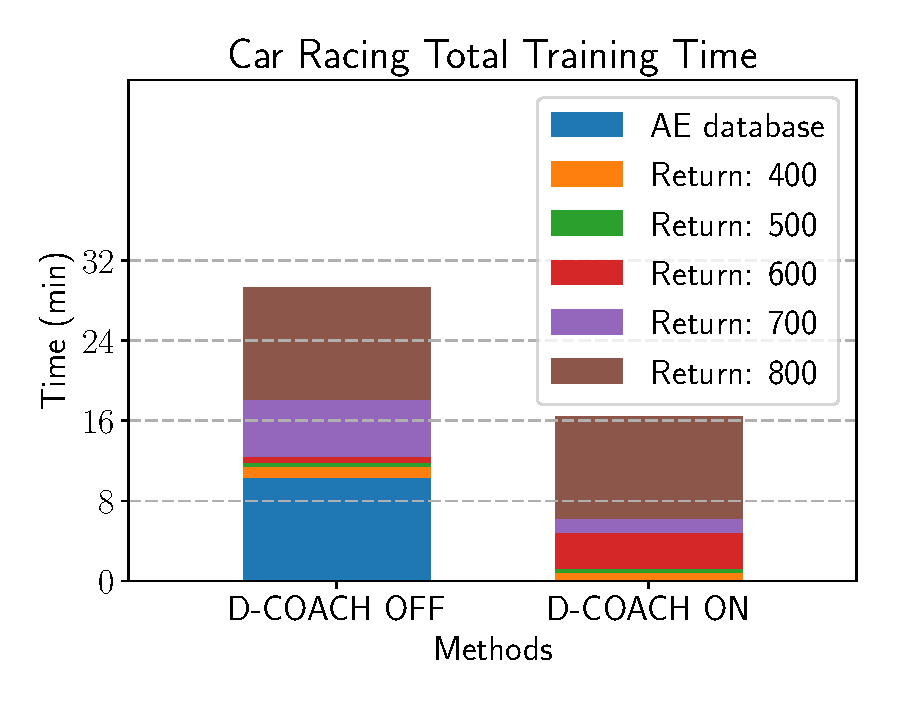
\includegraphics[width=0.5\linewidth]{imagenes/cap3/bar_car_racing_ICRA.pdf}}
\subfloat[][Duckie Racing.]{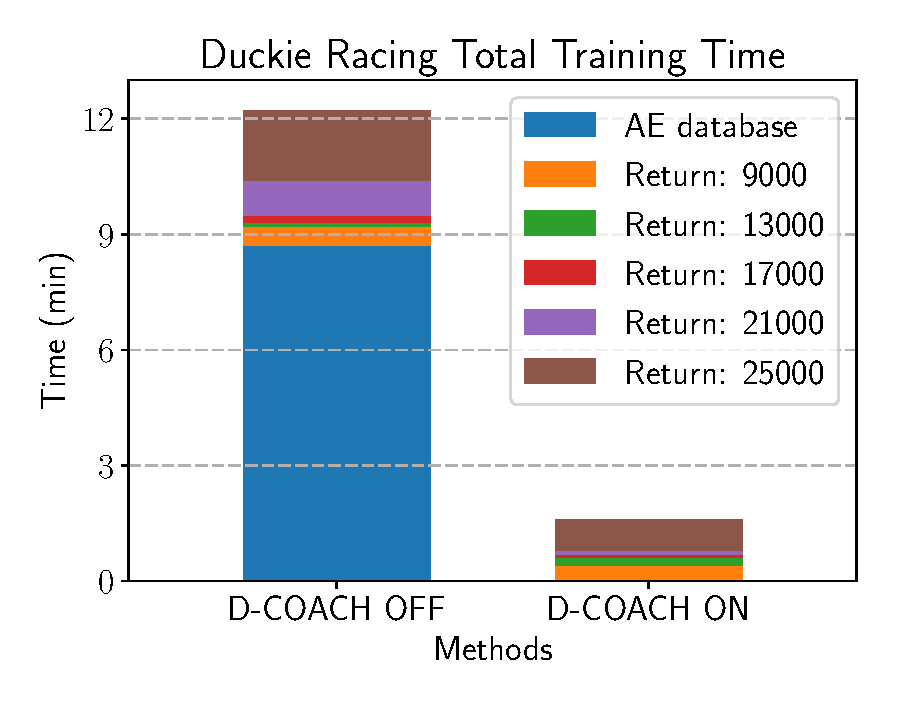
\includegraphics[width=0.5\linewidth]{imagenes/cap3/bar_duckie_ICRA.pdf}}
\caption{Comparison of the average human time dedicated to reach some levels of return.} 
\label{fig:stacked_bar} 
\end{figure}

\begin{figure}[H]
    \centering
    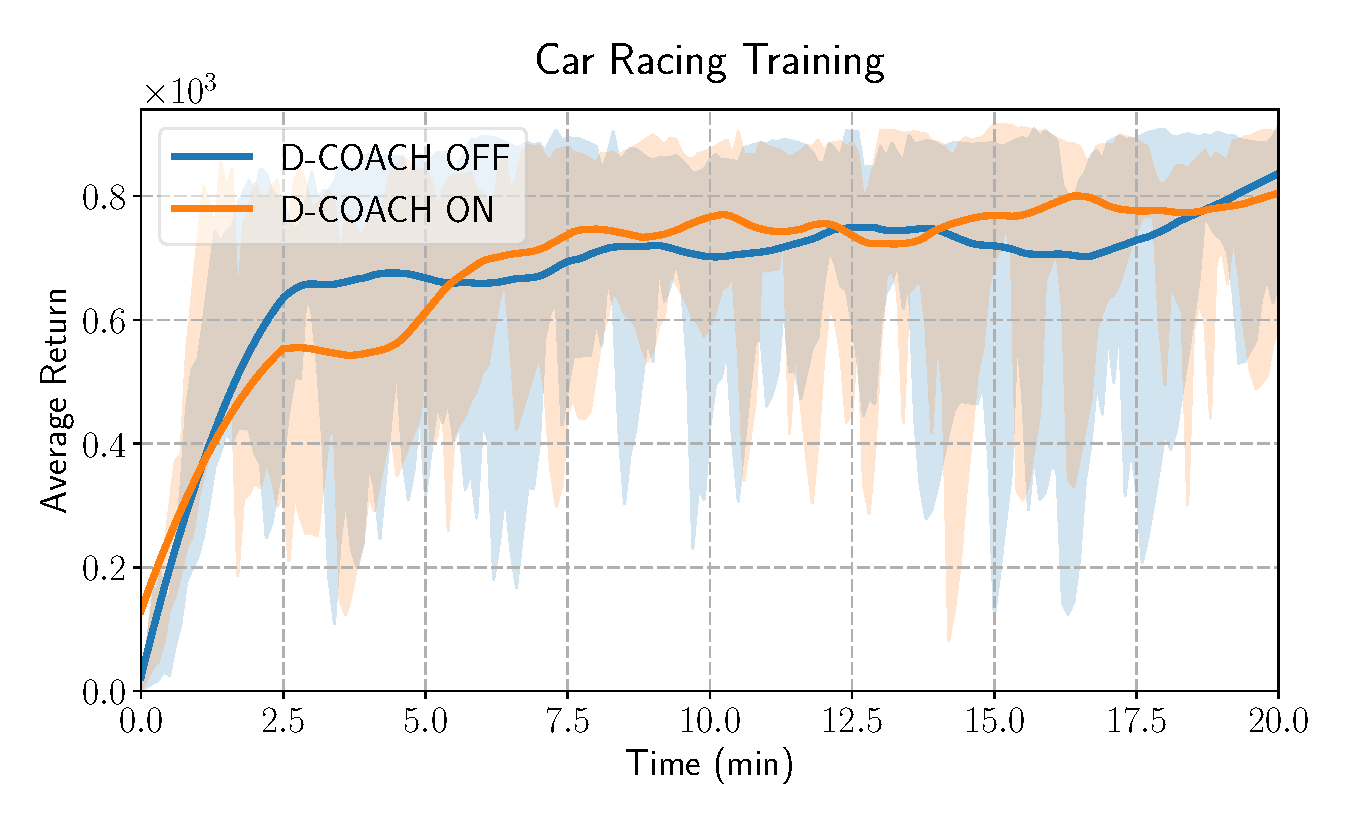
\includegraphics[width=0.9\linewidth]{imagenes/cap3/car_racing_human_teacher_ICRA.pdf}
    \caption{Results of learning with human teachers. Buffer: $K = 1000$; $b = 10$; $N = 8$.}
    \label{fig:humanteachers1}
\end{figure}

\begin{figure}[H]
    \centering
    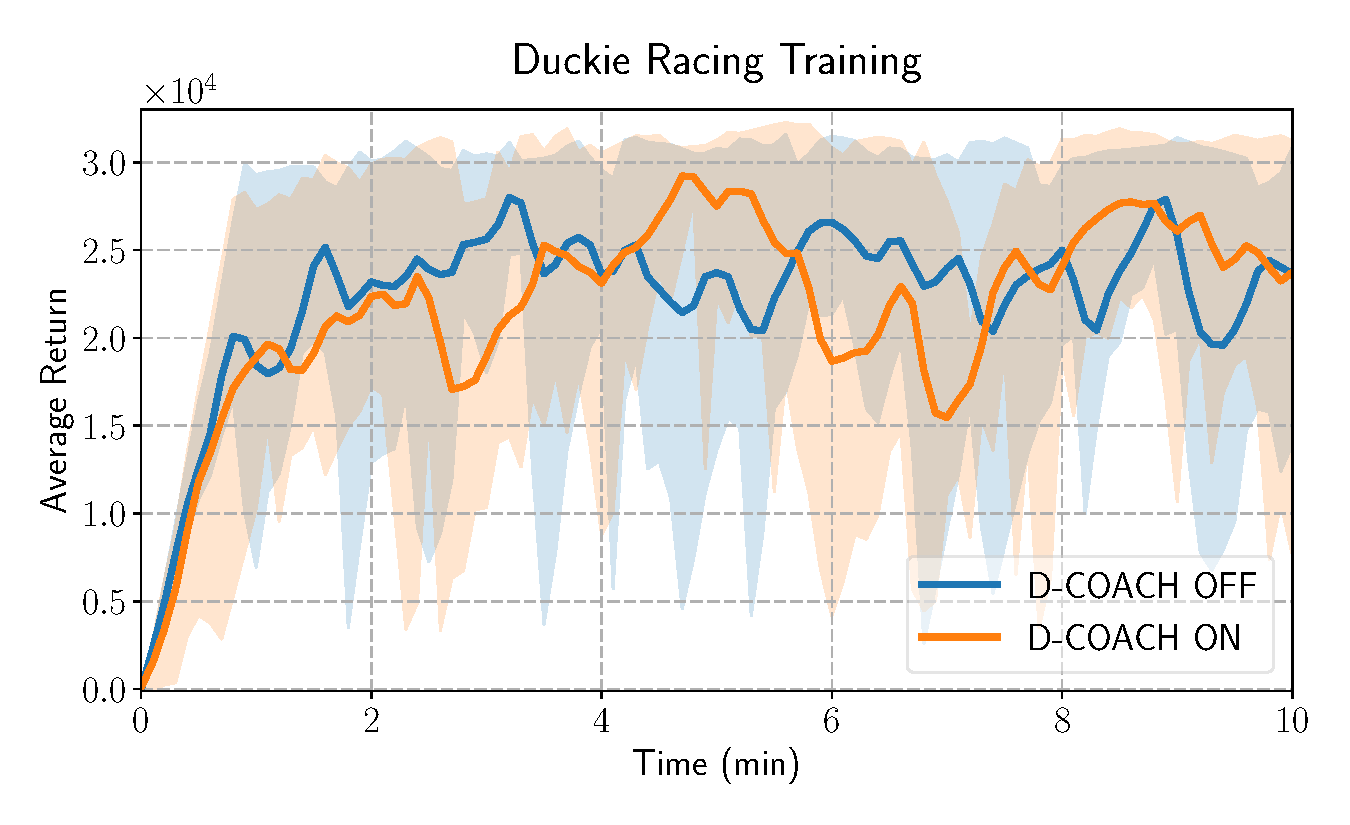
\includegraphics[width=0.9\linewidth]{imagenes/cap3/duckie_human_teacher_ICRA.pdf}
    \caption{Results of learning with human teachers. Buffer: $K = 1000$; $b = 10$; $N = 8$.}
    \label{fig:humanteachers2}
\end{figure}

\subsection{Additional validation with real systems}

Additional experiments with human teachers interacting with real robots through D-COACH v2 were carried out. These tests are for validating the results obtained with the previous two types of experiments, and no comparisons are presented.

A real Duckiebot was used for validating the results obtained with the simulations. An experienced teacher advised the policy of Duckiebot from scratch and obtained a good policy in six minutes (experiment available in \url{https://youtu.be/i4f1D4CH26E}). Similarly, in the pusher/reacher problems well performing policies were obtained within twenty minutes. 

Fig.~\ref{fig:reacher_exp} shows an extra validation that was done for the reacher case. A cost function was defined as the Euclidean distance between the end-effector of the arm and the object to track, normalized with the largest possible distance within the image (distance of opposite corners). Seven training sessions of 15 minutes were run and averaged. It is possible to observe that the cost decreases as the learning process advances. 

\begin{figure}[H]
    \centering
    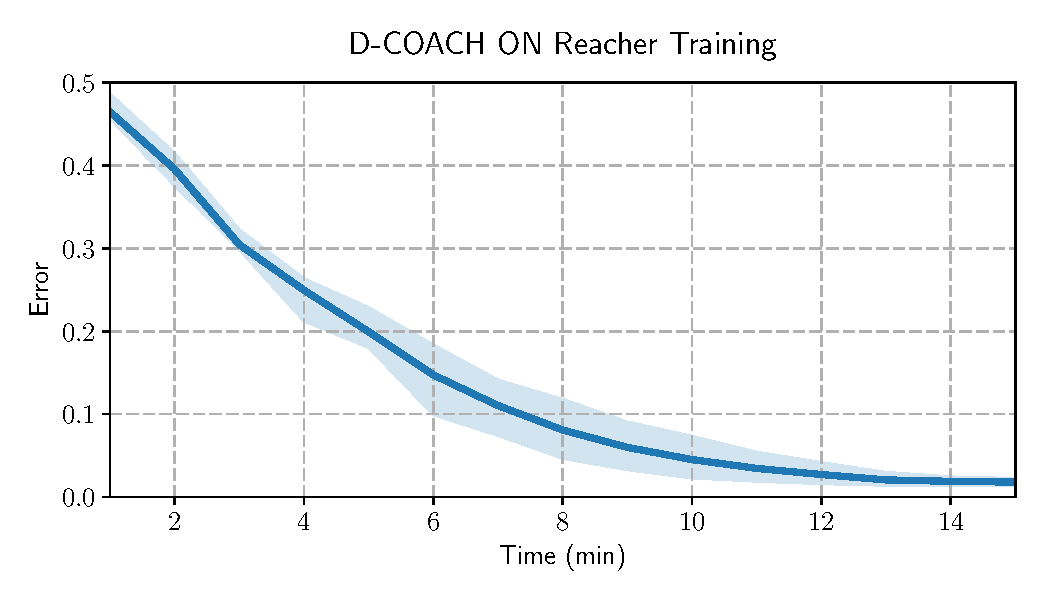
\includegraphics[width=0.9\linewidth]{imagenes/cap3/reacher_ICRA.pdf}
    \caption{Evolution of the error while learning the reacher task. }
    \label{fig:reacher_exp}
\end{figure}

\section{Discussion}

In this chapter we introduced an improved version of an interactive method for training policies represented with deep neural networks, particularly for problems wherein the observed state is defined in a high-dimensional space like a raw image.

The proposed D-COACH v2 offers a simpler learning scheme of only one step in which state representation and the policy itself are learned jointly using the two optimization criteria (the AE cost and the regression error of the policy). This method eliminates the necessity of recording demonstrations for the pre-training of the AE, which is a time consuming effort for the user, and sometimes is not possible due to complexity of the problem and lack of complex skills of the user in the task domain. In the approached problems, the effort of the users was reduced between $45\%$ and $80\%$. D-COACH v2 can adapt and extract features to represent reached unknown states during the learning process, which would be problematic for its basic version. Additionally, computational effort is reduced with the possibility of skipping the offline training of the AE, which is usually expensive. 

This simultaneous method is very data efficient for training the state representation. The AE is trained with the data gathered when human teachers advise corrections, which ensures a very representative database. Those samples correspond to the most important regions of the state space wherein the policy needs to discriminate different actions to execute.

The results also show that the interactive method can obtain higher performances than DRL in very few episodes. The level of the performance achieved by the interactive method would be obtained by DRL agents after several hundreds or thousands of episodes, which means that our proposed method is actually feasible, for learning with real robots in many applications wherein RL is not yet.
\chapter{Adding Memory to the Agents}
\section{Overview}
In the previous chapters, we have assumed that the agents interact in fully observable problems, following an MDP. This means that the observation that the agent receives from the environment is sufficient to fully understand its state. Thus:

\begin{equation}
    s_{t} = o_{t}
\end{equation}

But this is not always true. In robotics problems, robots observe its environment through sensors, and, commonly, the data obtained from them gives partial information about the robot's state. So, a significant set of real-world problems is better described by POMDPs.

There are different reason of why a problem could be partially observed. One of them is when a state is described by time-dependent phenomena, and the observations only get partial information about them. For instance, an agent could need to estimate the velocity of a flying drone by getting instant RGB snapshots of its movements. Unless observations from different time steps are combined, the agent is not going to be able to make this estimation. Other examples of time-dependent phenomena that do not have to do with the dynamics of the environment are temporary occlusions or corrupted communication systems between the sensors and the agent. From now on, we are going to use the acronym POMDP to refer to the just mentioned set of POMDPs.

All of these scenarios are not covered by the variations of D-COACH proposed so far. In this chapter, we aim to add memory to the policies trained with D-COACH, in order to have a system capable of solving sequential decision-making problems with partially observed time-dependent states. The idea is to validate this approach through simulations, establishing a baseline for further research in memory-based deep interactive learning.
\newpage

\section{Methodology}
There are two well-known approaches for adding memory to agents in sequential decision-making problems when using DNNs as function approximators:

\begin{enumerate}
    \item \textbf{Observation stacking \cite{atari}}: This approach consists in stacking a fixed number of past observations to the current one and using this stack as the input of the policy. 
    \item \textbf{Recurrent models \cite{hausknecht2015deep}:} This approach consists in using policies with RNN layers. Given that these models have an internal state, they can store information from the past (i.e. they have memory) and use it in future inferences. 
\end{enumerate}

One of the main issues of observation stacking is that the memory of these models is determined by the number of stacked observations. Problems that need to remember events in medium or large sequences would require larger stacks. In high-dimensional state problems, the size of the input can increase considerably as the number of stacked observations increments, generating high overheads. In contrast, RNN-based models have the ability to remember information for an arbitrarily long amount of time \cite{lample2017playing}.  Also, they have no input-related overheads because when these models are evaluated they are fed with one observation at a time. In RNNs, the memory-related overhead is determined by the size of their hidden states and the length of the sequences used when updating the weights of the models (so the latter is only effective when training).

From an engineering point of view, using RNNs in products for real-world applications with long or medium time dependencies could lower their costs in comparison to using observation stacking. The input overhead of approaches based on stacked observations would be too high in these scenarios; thus, more powerful (expensive) computers would be needed. 

Given the more practical usage of recurrent models and their capability of remembering arbitrarily long sequences, in this chapter we use RNN-based policies (with LSTM layers) to test the viability of D-COACH for solving problems in POMDP settings. 

\subsection{Learning to Remember}
Even though RNNs are networks with the capability of storing/embedding information from past observations, they have to learn to do this. Commonly, in DRL approaches this is implicitly learned when backpropagating the error that aims to maximize the expected return. This gives the intuition that when using D-COACH, backpropagating the correction error through the recurrent layers should be enough for learning well-performing policies. Nevertheless, preliminary tests showed that shaping recurrent models with corrective feedback made the agents to rapidly overfit to the first set of corrections, loosing the capability of learning interesting behaviors and, as a consequence, solving tasks. 

To overcome this shortcoming, we propose to have DNNs separated into two parts: (1) transition model and (2) policy. The transition model is in charge of learning the dynamics of the environment in a supervised manner using samples collected by the agent while the policy part is shaped using corrective feedback. 

In MDPs, a transition model is capable of predicting the next state of the environment as a function of the current state and the taken action $M(s_{t},a_{t}) = s_{t+1}$ (as in Equation \ref{eq:model}). In contrast, in POMDPs the agent does not have direct access to its state, so, instead, the transition model can be trained to predict the next observation $o_{t+1}$. To achieve this, the neural network architecture must include recurrent layers (LSTMs in this case). LSTMs are capable of embedding in their hidden state $h_{t}$ information from past observations, which is crucial to predict the next observation when the environment is partially observed. Thus, the objective of the first part of the DNN is to learn $M(o_{t},a_{t}, h_{t-1}) = \widetilde o_{t+1}$, which, as a consequence, learns to embed past observations in $h_{t}$.

The second part of the DNN, the policy, takes as input the concatenation of the hidden state of the transition model computed in the last time step $h_{t-1}$ with the current observation of the environment $o_{t}$ and uses this information as if it were the state. D-COACH is used to update the weights of this part as it is done in fully-observable low-dimensional state problems with D-COACH OFF. In this chapter, we are assuming that an embedding of past observations combined with the current observation is a good approximation of $s_{t}$:

\begin{equation}
s_{t}\approx (h_{t-1}, o_{t})    
\end{equation}

We call this approach Memoryful ONline state representation learning D-COACH (D-COACH MON). A summary of this approach is presented in Figure \ref{fig:mb_dcoach}.

\begin{figure}[h]
    \centering
    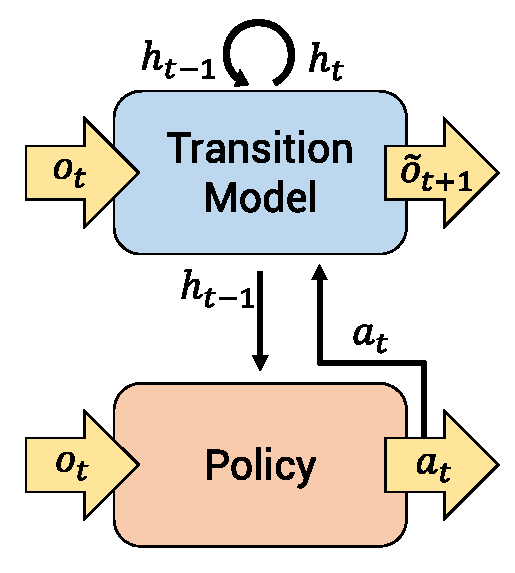
\includegraphics[width=0.4\linewidth]{imagenes/cap4/model_based_dcoach.pdf}
    \caption{D-COACH MON general structure.}
    \label{fig:mb_dcoach}
\end{figure}

\newpage

\subsection{Low-dimensional State with Memory}
\label{sec:ld_memory}
As it has been done previously in this work, we first study the low-dimensional state case. The objective is to learn the dynamics of the environment online i.e. as the policy is shaped interactively. 

If we look back to the approach taken in Chapter 3, the idea was similar. In that case the objective was to learn a low-dimensional embedding of a high-dimensional input online. The strategy was to share the encoder layers of an autoencoder between the policy and the autoencoder, and to update them using both the cost of the policy and the one of the autoencoder. In this case, the hidden state of the LSTM could be interpreted as an embedding of past observations. So, this recurrent layers could be shared between the policy and the model, updating them using both costs. A simplified version of this approach is shown in Figure \ref{fig:ld_model_rip}.

\begin{figure}[h]
    \centering
    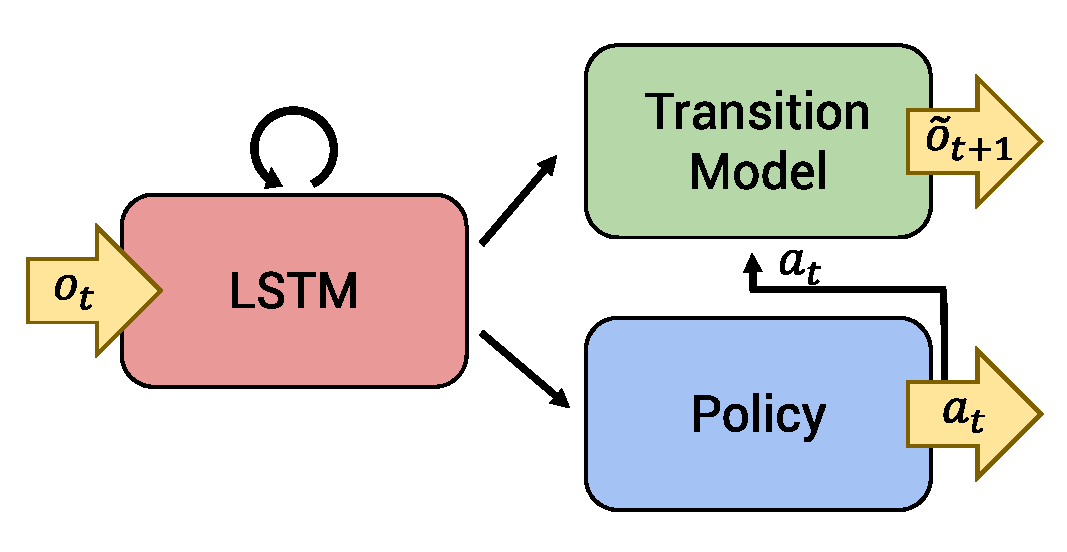
\includegraphics[width=0.6\linewidth]{imagenes/cap4/ld_model_rip.pdf}
    \caption{Low-dimensional observations general neural network architecture for POMDPs (option 1).}
    \label{fig:ld_model_rip}
\end{figure}

The shortcoming presented in the approach shown in Figure \ref{fig:ld_model_rip} is that in this case the same problem that we found in the preliminary tests appears. The error of the policy does not work well when updating the weights of recurrent layers using the D-COACH strategy, even when using the auxiliary cost of the model. 

Alternatively, the approach that was finally taken was to update the model and the policy separately and simultaneously. If we go back to Figure \ref{fig:mb_dcoach}, this would mean that the \textbf{Transition Model} box is updated with transitions collected by the agent, and, separately, the \textbf{Policy} box is updated with corrective feedback. The proposed transition model architecture (\textbf{Transition Model} box in Figure \ref{fig:mb_dcoach}) consists on LSTM and FNN layers, as shown in Figure \ref{fig:ld_model_win}. The policy architecture (\textbf{Policy} box) is simply a composition of FNN layers, as it is done in the other variations of D-COACH.

\newpage

\begin{figure}[H]
    \centering
    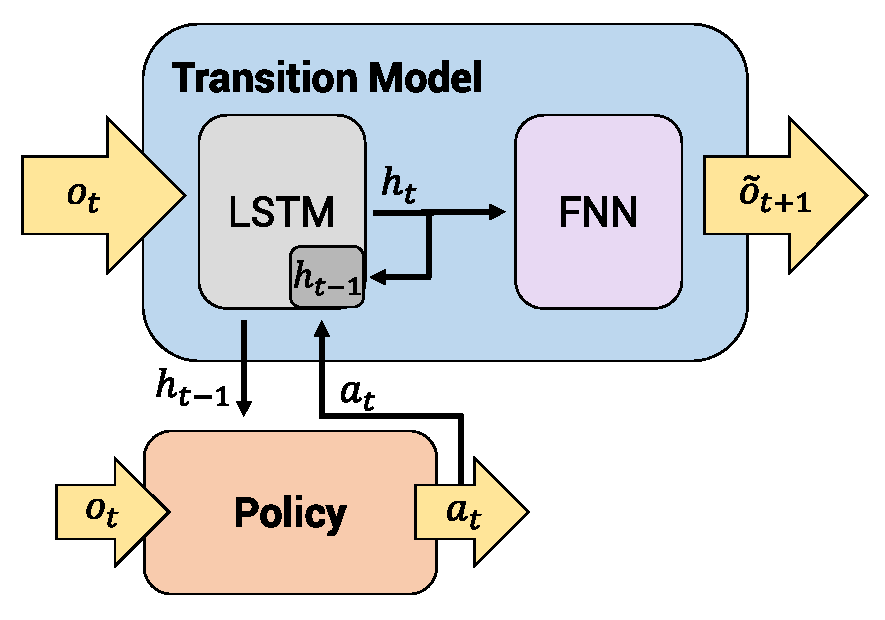
\includegraphics[width=0.5\linewidth]{imagenes/cap4/ld_model.pdf}
    \caption{Low-dimensional observations general neural network architecture for POMDPs (option 2).}
    \label{fig:ld_model_win}
\end{figure}

Figure \ref{fig:ld_model_win} presents the general structure of the neural network architecture that is proposed for problems with low-dimensional observations. A detailed version of the network architecture is provided in Figure \ref{fig:detailed_ld}.

\begin{figure}[h]
    \centering
    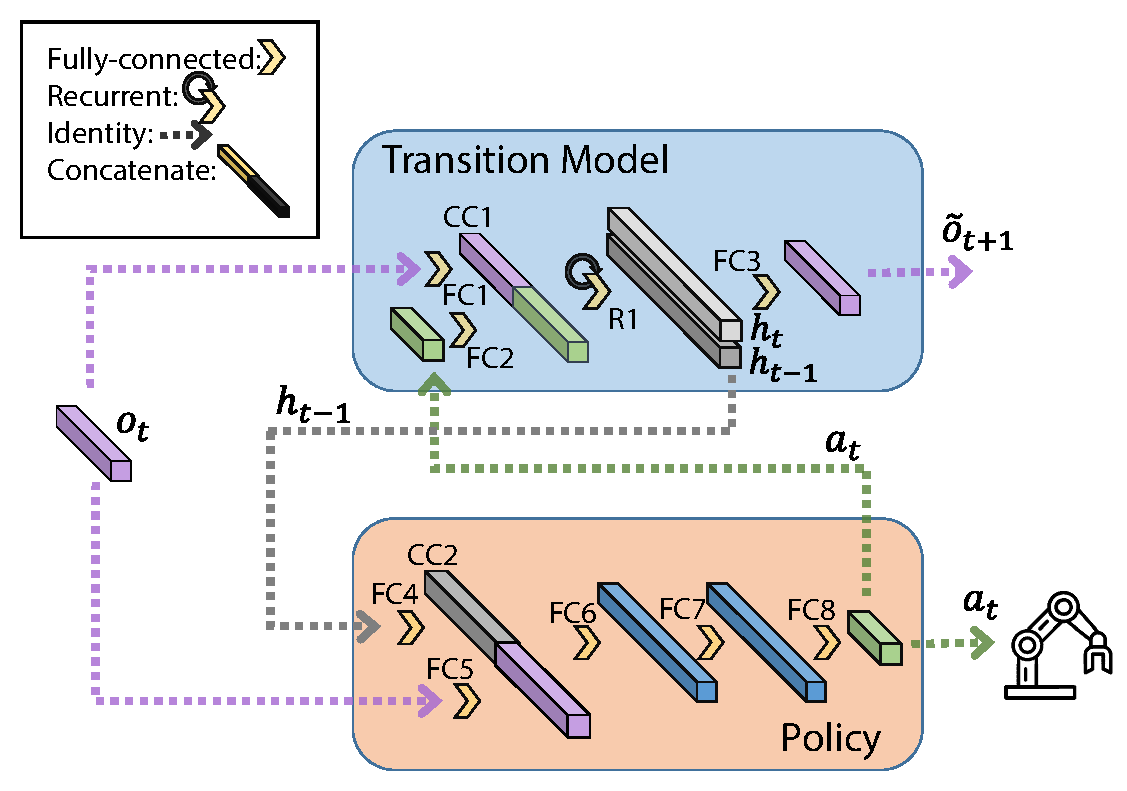
\includegraphics[width=0.8\linewidth]{imagenes/cap4/ld_model_det.pdf}
    \caption{D-COACH MON low-dimensional observations neural network architecture.}
    \label{fig:detailed_ld}
\end{figure}

As mentioned before, the transition model and the policy are trained as two separate networks. These networks depend on each other. The policy uses as part of its input $h_{t-1}$, which is a vector that the transition model outputs. Similarly, the transition model uses the last taken action as part of its input, which is a vector generated by the policy. When an update of the architecture is done, the transition model is first updated, and, consecutively, the policy is updated. A summary of this process is presented in Figure \ref{fig:ld_mon_train}.

\begin{figure}[h]
\centering
\subfloat[][Transition model update step.]{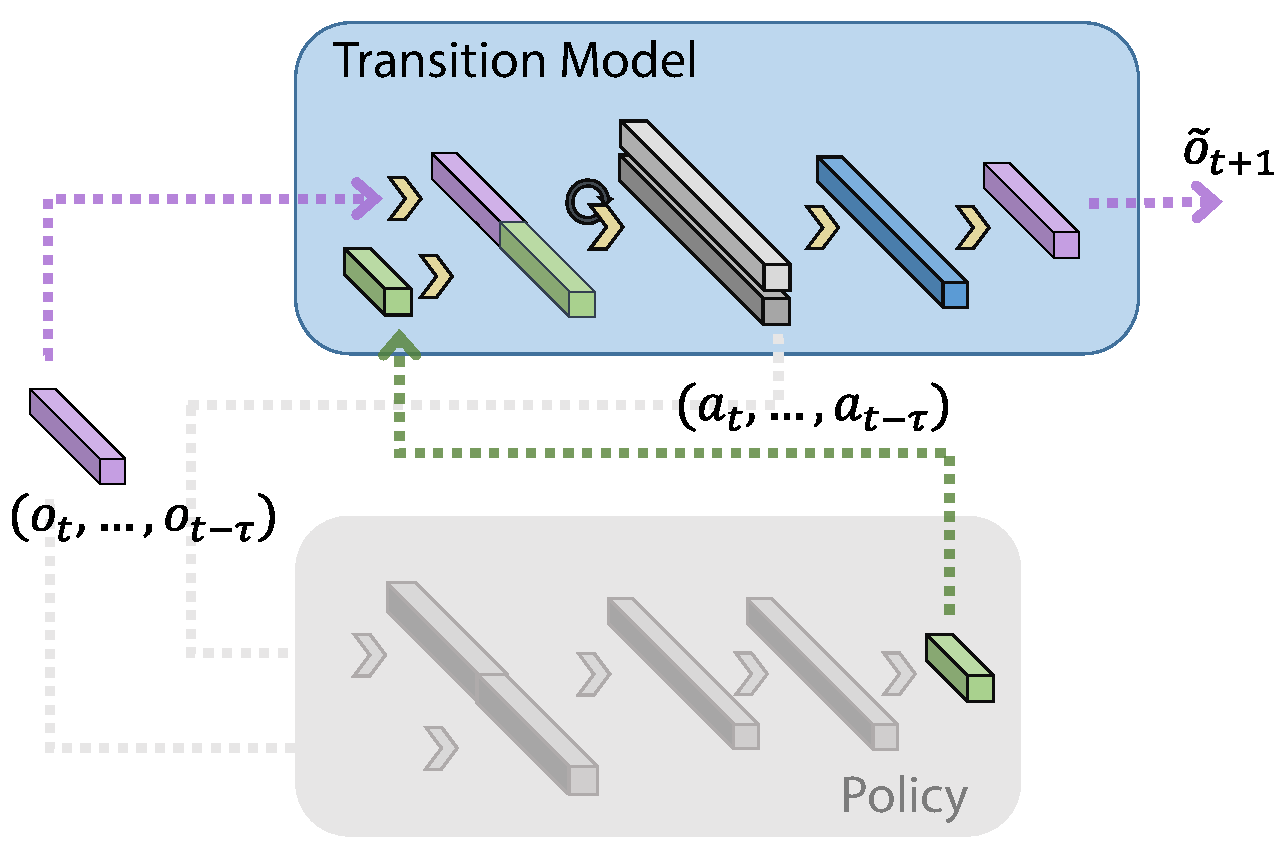
\includegraphics[width=0.45\linewidth]{imagenes/cap4/ld_mon1.pdf}}
\subfloat[][Policy update step.]{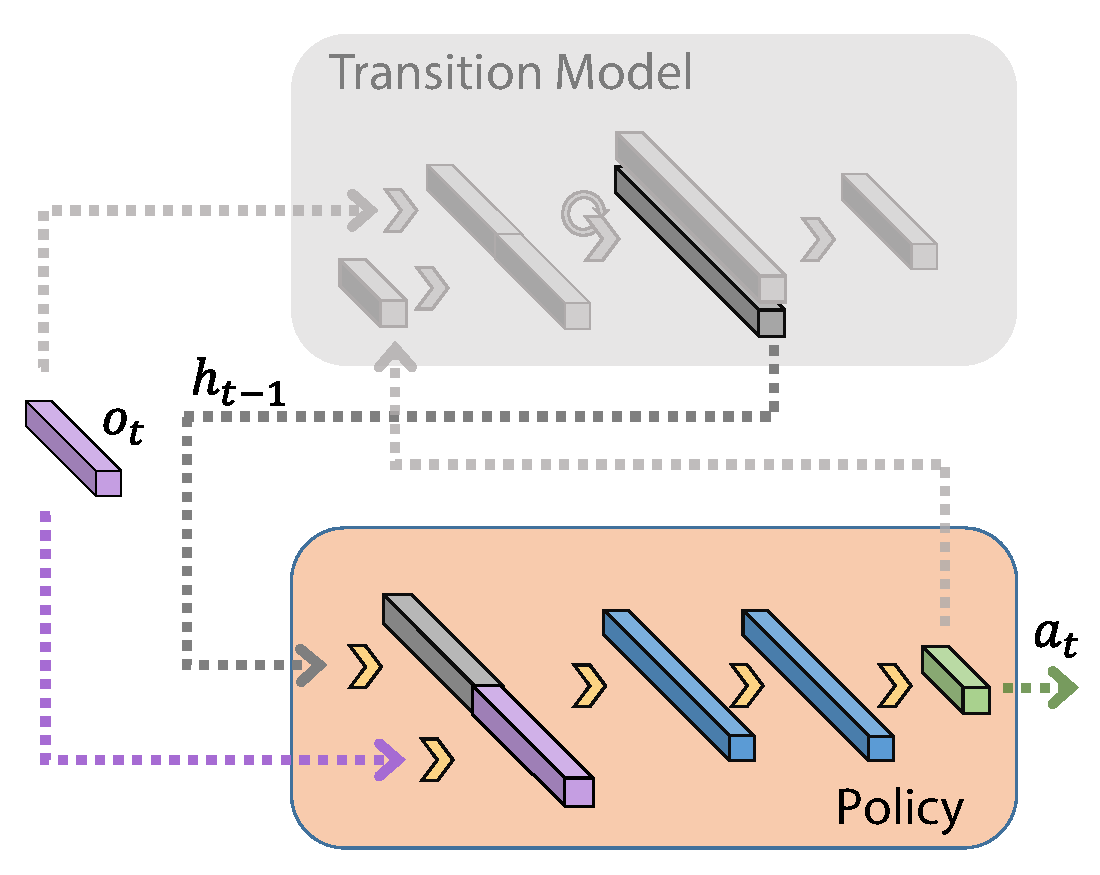
\includegraphics[width=0.45\linewidth]{imagenes/cap4/ld_mon2.pdf}}
\caption[Update step of D-COACH MON neural network for low-dimensional observations.]{Update step of D-COACH MON neural network for low-dimensional observations. First (a), the transition model is updated in a supervised manner using as input a batch with sequences of observations and actions where the labels correspond to $o_{t+1}$. Consecutively (b), the policy is updated using human corrective feedback using as input $o_{t}$ and $h_{t-1}$.} 
\label{fig:ld_mon_train} 
\end{figure}

\subsection{High-dimensional State with Memory}
In the high-dimensional case, agents need to learn two embeddings: (1) spatial and (2) temporal. Spatial embeddings are understood as a low-dimensional representation of high-dimensional data, which is what it has been covered in the former chapters using autoencoders. In contrast, temporal embeddings refer to encapsulating previous observations in a memory, which is what it has been done in Section \ref{sec:ld_memory} using LSTMs. 

In preliminary tests, we found that the most effective way of doing this under the setting of D-COACH is to treat the autoencoder and the recurrent layers as one architecture to represents the transition function model. A model with the capability of learning from high-dimensional states, as it can be seen in Figure \ref{fig:rnn_hd}. 

\begin{figure}[h]
    \centering
    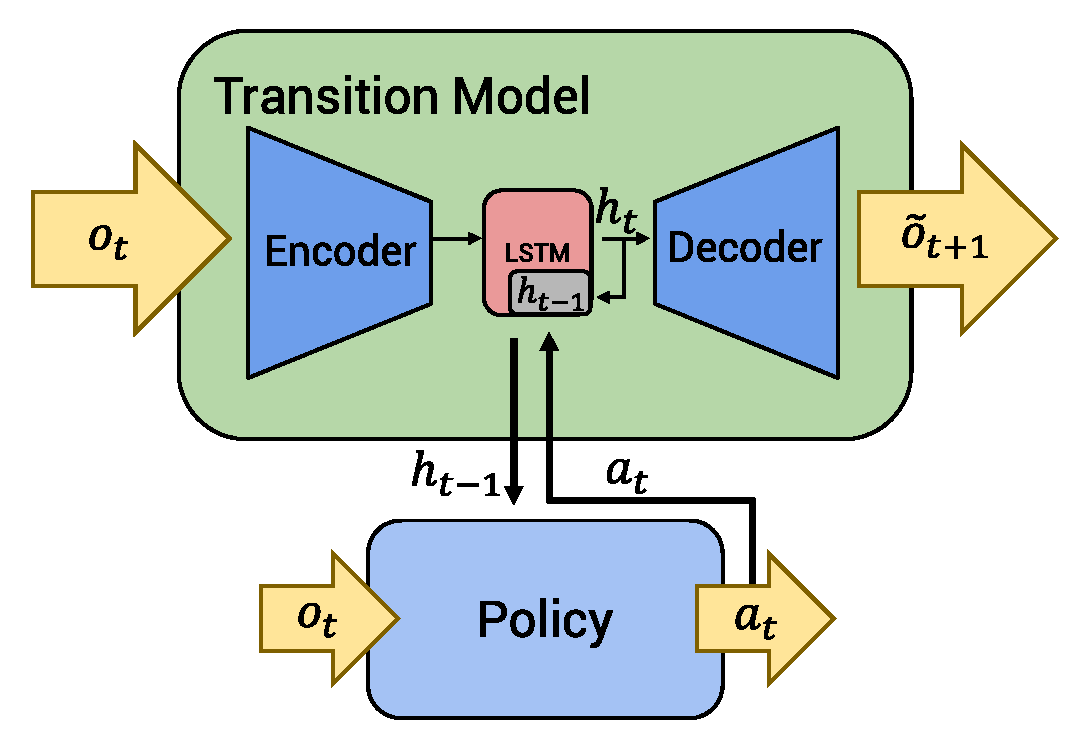
\includegraphics[width=0.5\linewidth]{imagenes/cap4/hd_model.pdf}
    \caption{High-dimensional observations general neural network architecture for POMDPs.}
    \label{fig:rnn_hd}
\end{figure}

Instead of using separate costs for the model and the autoencoder, the autoencoding cost for reconstructing $o_{t+1}$ is used. So, Equation \ref{eq:ae} instead of being $L(x_{t},\widetilde x_{t})$ it would be  $L(x_{t},\widetilde x_{t+1})$. By doing this, the hidden state of the LSTM embeds both the high-dimensional input and past observations, given that the autoencoder tries to reconstruct and predict $o_{t+1}$. As it was done for the low-dimensional observation case, Figure \ref{fig:detailed_hd} introduces the detailed neural network architecture for the high-dimensional observation case.

\begin{figure}[h]
    \centering
    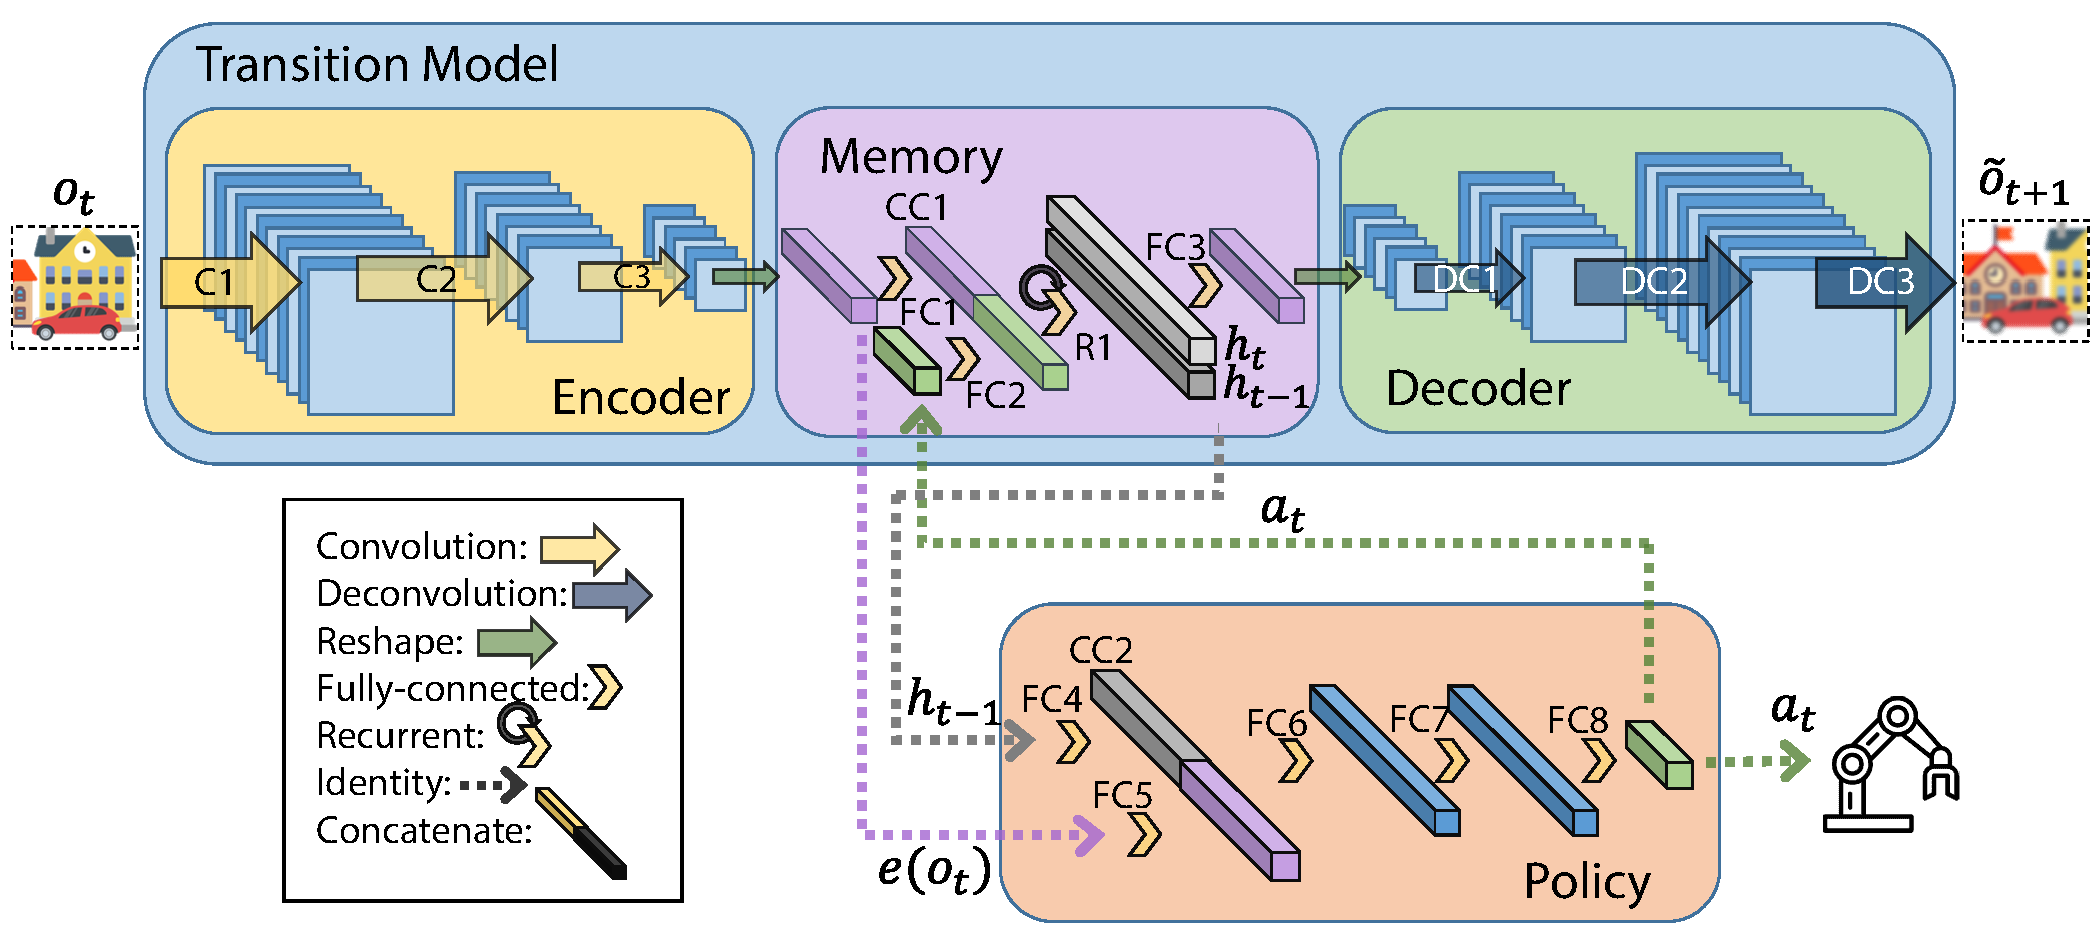
\includegraphics[width=\linewidth]{imagenes/cap4/hd_model_det.pdf}
    \caption{D-COACH MON high-dimensional observations neural network architecture.}
    \label{fig:detailed_hd}
\end{figure}

In the same way as in the low-dimensional observation case, the transition model and the policy are trained separately and simultaneously. The only difference is that in this case, when the policy is updated it uses the encoding layers to generate an encoded low-dimensional representation of the observation $e(o_{t})$ that the policy uses as input, but only the policy layers are updated. This is also different from what is done in D-COACH OFF, where the encoding layers are also updated when training the policy. Figures \ref{fig:hd_mon_train1} and \ref{fig:hd_mon_train2} summarize a D-COACH MON update step for high-dimensional observations.

\begin{figure}[h]
    \centering
    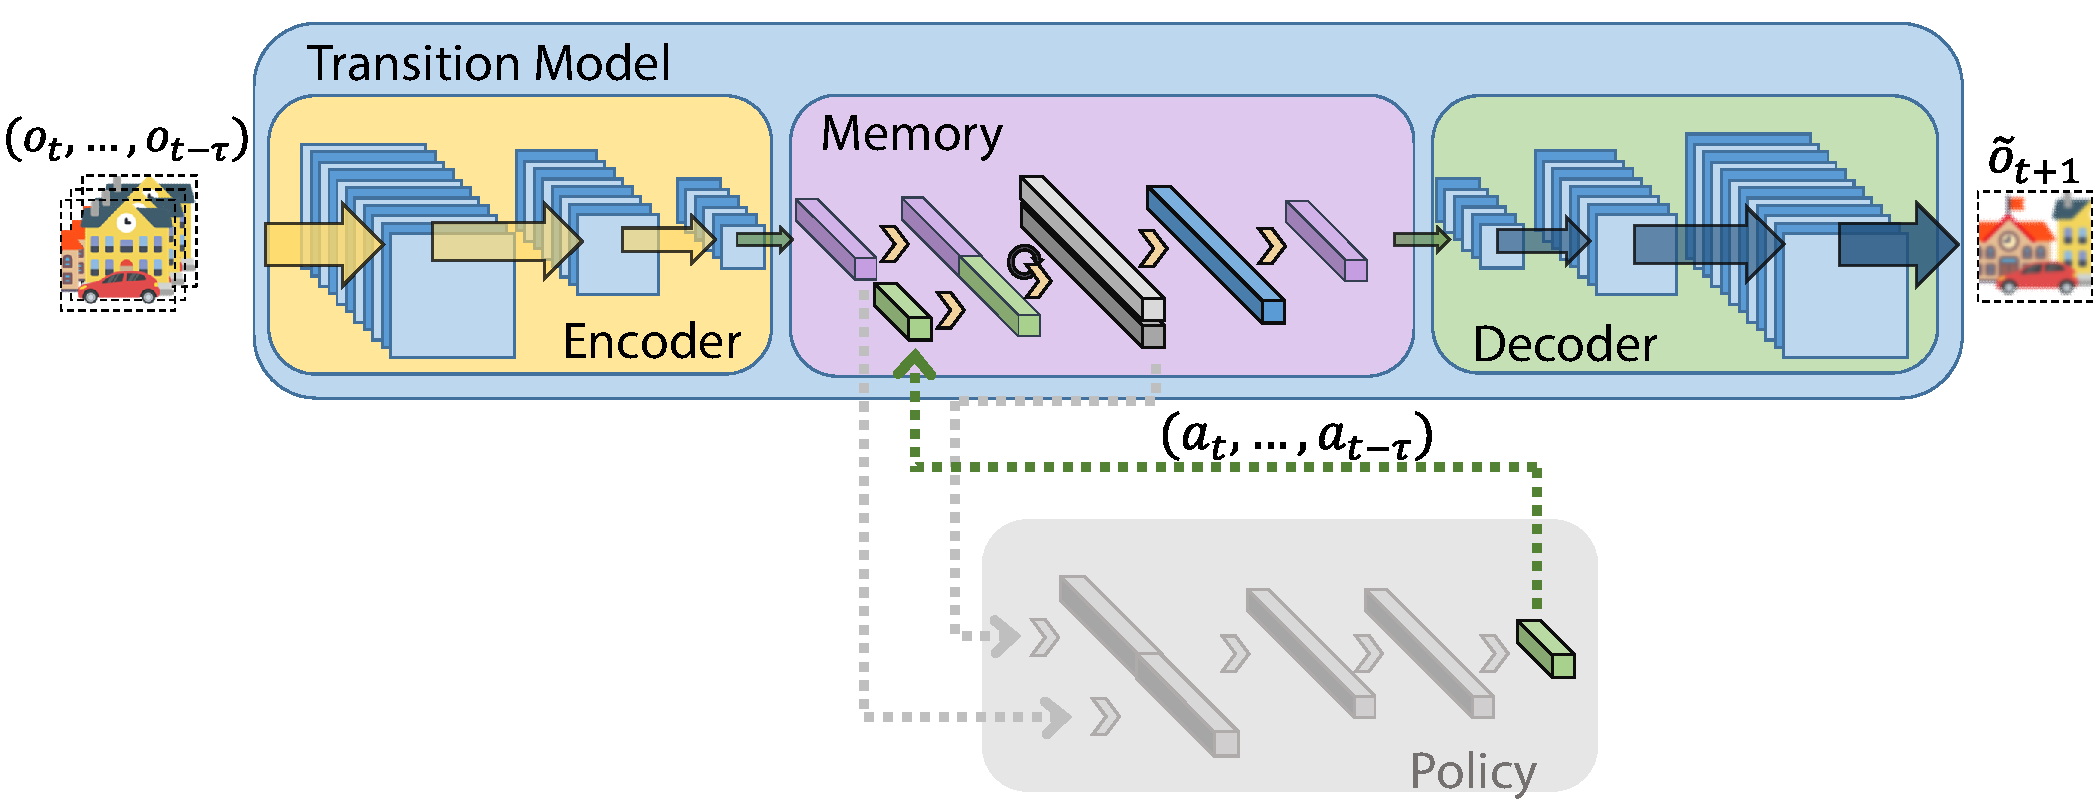
\includegraphics[width=0.93\linewidth]{imagenes/cap4/hd_mon1.pdf}
    \caption{Transition model update step.}
    \label{fig:hd_mon_train1}
\end{figure}

\begin{figure}[h]
    \centering
    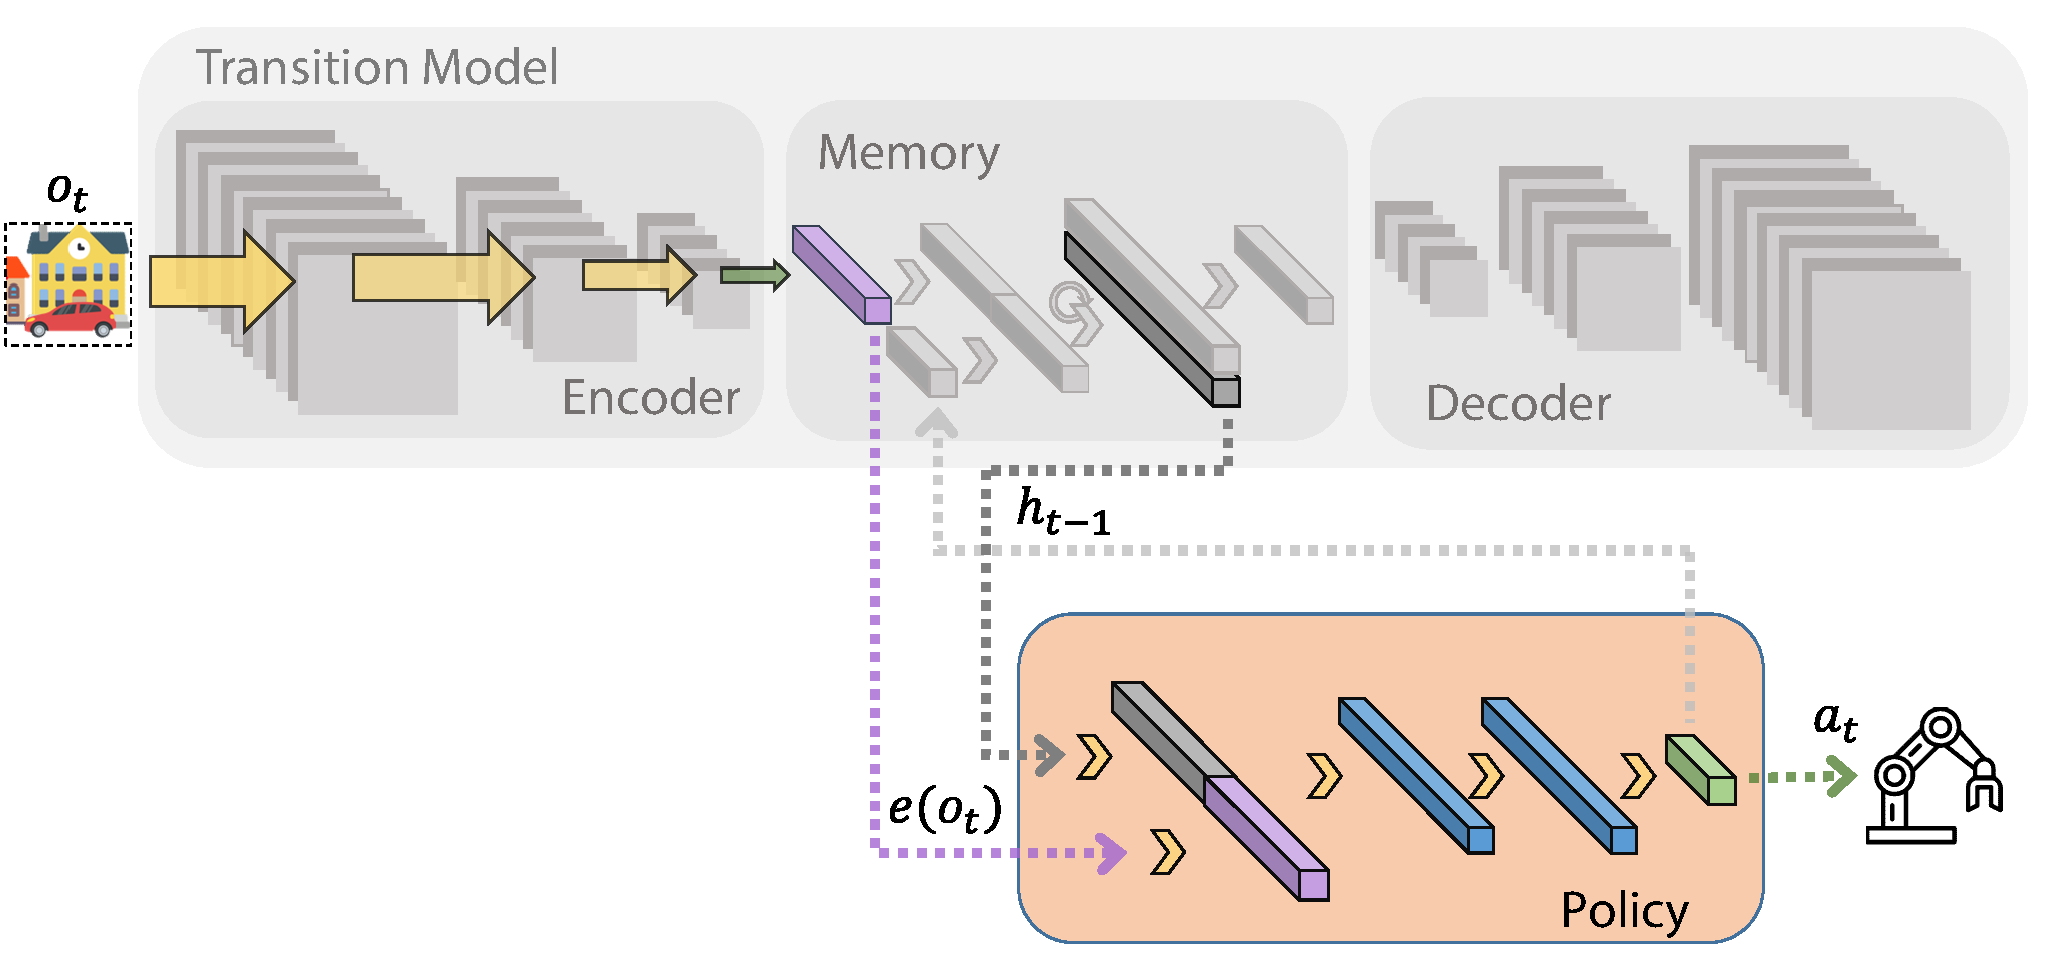
\includegraphics[width=0.93\linewidth]{imagenes/cap4/hd_mon2.pdf}
    \caption{Policy update step.}
    \label{fig:hd_mon_train2}
\end{figure}


\subsection{The Algorithm}

In Algorithm \ref{algorithm:DeepCOACH-M}, the pseudocode of D-COACH MON is presented. The hidden state of the LSTM is denoted as  $h^{\mathrm{LSTM}}$ and the human corrective feedback as $h$.

 In every time step, the agent executes an action based on its last observation and in the current hidden state of the LSTM (line 5). This hidden state is updated using its previous value and the most recent observation and action (line 7). In this occasion, a buffer in charge of storing the samples of the transition function model ($\mathcal{D}$) is incorporated. In both buffers, $\mathcal{B}$ and $\mathcal{D}$, sequences with length $\tau$ are stored (lines 8 and 18), which is necessary for training the LSTM. This is done following the \emph{bootstrapped random updates} \cite{hausknecht2015deep} strategy. As in the former versions of D-COACH, $\mathcal{B}$ is used for updating the policy (lines 16 and 22) by replaying past corrections. In contrast, $\mathcal{D}$ replays past transitions of the environment in order to update the transition function model (lines 17 and 24). The transition model is updated every time feedback is given (lines 15 and 17), in the same way as it is done with the policy in all of the variations of D-COACH, including this one (lines 14 and 16). 

\begin{algorithm}[H]
\caption{D-COACH MON: Memoryful Online State Representation Learning}\label{algorithm:DeepCOACH-M}
\begin{algorithmic}[1]
\State \textbf{Require:} error magnitude $e$, policy buffer update interval $b$, policy buffer sampling size $N$, policy buffer min. size $k$, policy buffer max. size $K$, model buffer update interval $d$, transition function model buffer sampling size $M$, transition function model buffer min. size $l$, transition function model buffer max. size $L$, training sequence length $\tau$.
\State \textbf{Init:} $\mathcal{B} = []$, $\mathcal{D} = []$
\For{t = 1,2,...}{}
\State \textbf{observe} observation $o_{t}$
\State \textbf{execute} action $a_{t}=\pi(o_{t}, h^{\mathrm{LSTM}}_{t-1})$
\State \textbf{feedback} human corrective advice $h_{t}$
\algstore{myalg}
\end{algorithmic}
\end{algorithm}

\begin{algorithm}            
\begin{algorithmic} [1]                  
\algrestore{myalg}
\State \textbf{compute} $h^{\mathrm{LSTM}}_{t}$ from $M(o_{t}, a_{t},h^{\mathrm{LSTM}}_{t-1})$
\State \textbf{append} $(o_{t-1},...,o_{t-\tau},a_{t-1},...,a_{t-\tau},o_{t})$ to $\mathcal{D}$
\If{length($\mathcal{D}$) $> L$ }
\State $\mathcal{D} = \mathcal{D}[2:L+1]$
\EndIf
\If{$h_{t}$ is not \textbf{0}}
\State $\mathit{error}_{t} = h_{t}\cdot e$
\State $y_{label(t)} = a_{t} + \mathit{error}_{t}$ 
\State \textbf{update} $\pi$ using SGD with $(o_{t}, h^{\mathrm{LSTM}}_{t-1}, y_{\mathit{label}(t)})$ 
\State \textbf{update} $M$ using SGD with $(o_{t-1},...,o_{t-\tau},a_{t-1},...,a_{t-\tau},o_{t})$
\State \textbf{update} $\pi$ using SGD with a mini-batch of sequences sampled from $\mathcal{B}$
\State \textbf{update} $M$ using SGD with a mini-batch of sequences sampled from $\mathcal{D}$
\State \textbf{append} $(o_{t},...,o_{t-\tau},a_{t-1},...,a_{t-\tau}, y_{\mathit{label}(t)})$ to $\mathcal{B}$
\If{length($\mathcal{B}$) $> K$ }
\State $\mathcal{B} = \mathcal{B}[2:K+1]$
\EndIf
\EndIf
\If{mod(t, b) is 0 and length($\mathcal{B}$) $\geq$ $k$}
\State \textbf{update} $\pi$ using SGD with a mini-batch of sequences sampled from $\mathcal{B}$
\EndIf
\If{mod(t, d) is 0 and length($\mathcal{D}$) $\geq$ $l$}
\State \textbf{update} $M$ using SGD with a mini-batch of sequences sampled from $\mathcal{D}$
\EndIf
\EndFor
\end{algorithmic}
\end{algorithm}


\section{Experiments and Results}
Simulated teachers were used in three different problems for validating D-COACH MON. The main idea behind these experiments is to compare D-COACH MON with D-COACH ON in partially observable problems.

\begin{enumerate}
    \item \textbf{Partially Observed Cart-Pole:} A partially observed low-dimensional state scenario. This is the same environment used in Chapter 2 with a modification in the observation space of the agent. In the standard fully-observable cart-pole the state has four dimensions, which consists of the position $x$ and velocity $\dot x$ of the cart and the angle $\theta$ and angular velocity $\dot \theta$ of the pole, such that $s=[x, \dot x, \theta, \dot \theta]$. In this case, we take out the derivatives present in the state, such that $s=[x, \theta]$.
    \item \textbf{Partially Observed Cart-Pole from Pixels:} The cart-pole environment is modified to use as input raw pixels with dimensions $32\times32\times1$(high-dimensional state). 
    \item \textbf{Partially Observed Car Racing:} A partially observed high-dimensional state scenario. The Car Racing problem presented in Chapter 2 is modified such that the indicators in the bottom of the image are no longer available (see Figure \ref{fig:no_inds_car_racing}). 
\end{enumerate}

\begin{figure}[h]
    \centering
    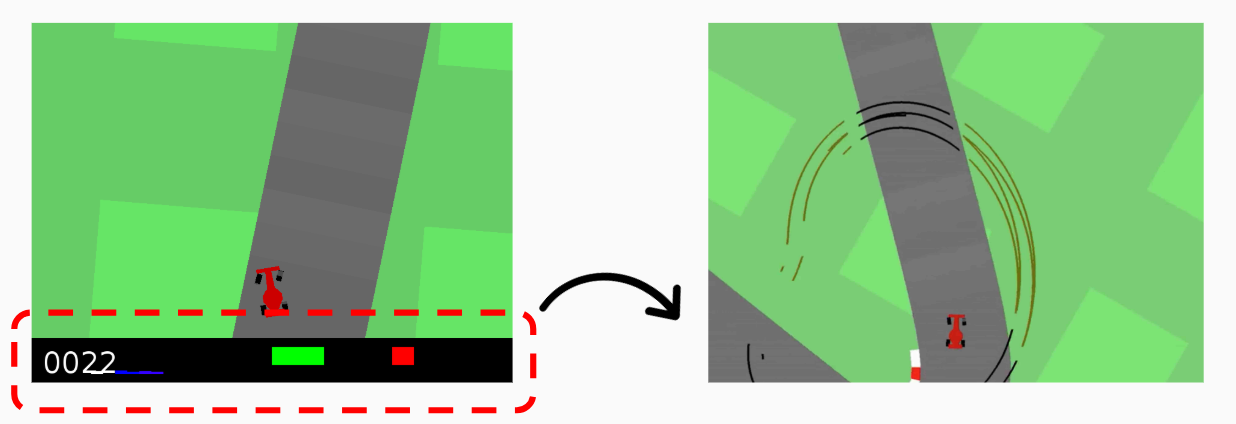
\includegraphics[width=0.8\linewidth]{imagenes/cap4/car_racing_no_inds.PNG}
    \caption{Partially observed Car Racing: indicators at the bottom of the observation are removed.}
    \label{fig:no_inds_car_racing}
\end{figure}

All the results that present averaged data in the form of a curve have confidence intervals that represent the $60^{th}$ percentile of the data. The same hyper-parameters introduced in Figure \ref{fig:network_diagram} were used. In addition an LSTM layer was added between the encoder and the decoder of the autoencoder (in problems with high-dimensional observations) were the dimensionality of $h^{LSTM}$ was $150$.

\subsection{Validation Low-Dimensional State}

D-COACH MON is tested in the partially observed cart-pole because it is a way of validating if the proposed methodology works in a simple setting. Figure \ref{fig:ld_cartpole_model} shows the learning curves of D-COACH MON and D-COACH ON. The same strategy used in Chapter 3 for training policies with a simulated teacher is employed in this section.

\begin{figure}[H]
    \centering
    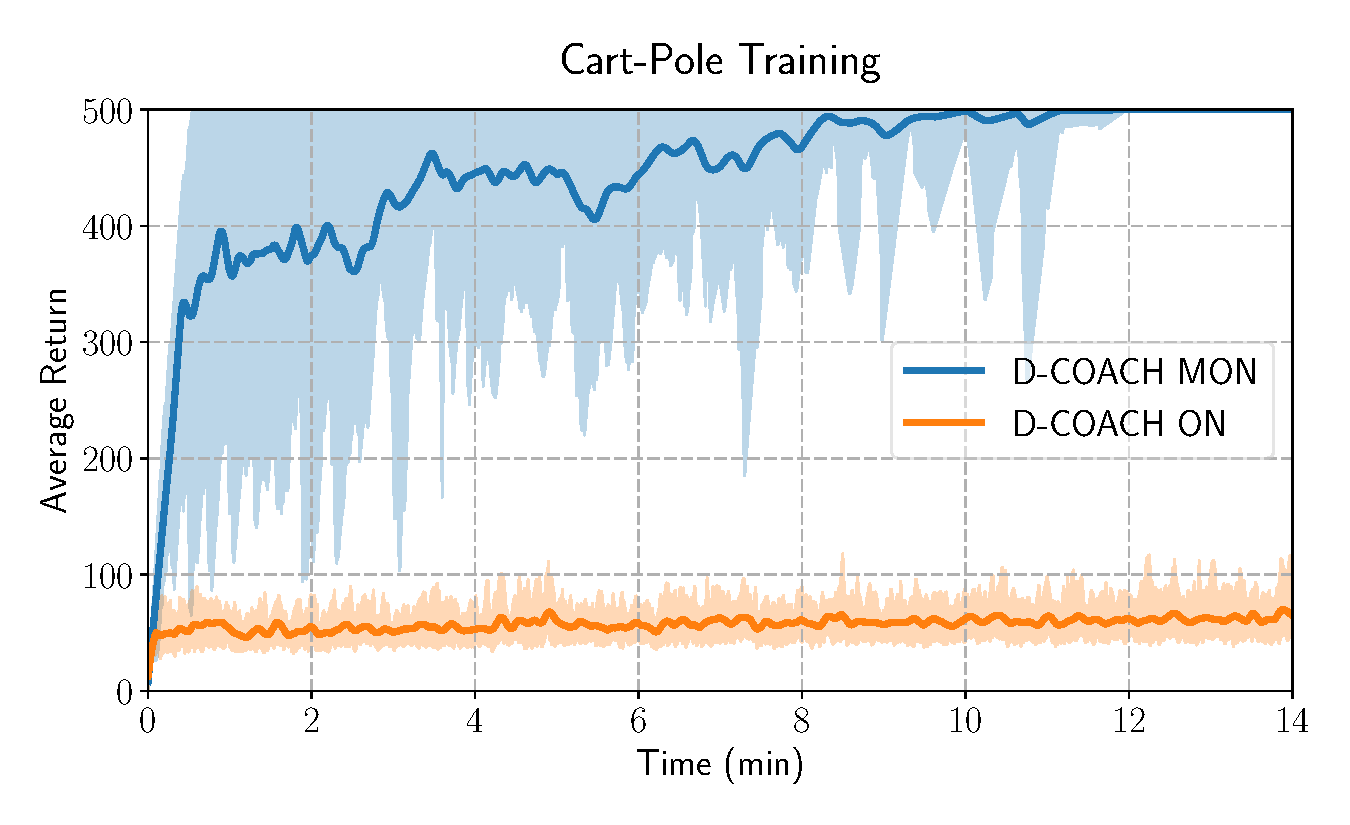
\includegraphics[width=0.8\linewidth]{imagenes/cap3/cartpole_LD_model.pdf}
    \caption{Partially observed cart-pole results for simulated teacher comparing D-COACH ON and D-COACH MON.  Buffer: $K = 200$; $k=5$; $b = 10$; $N = 50$; $L=1\mathrm{e}5$; $l=5$; $d=1$; $M=50$; $\tau=8$; $P_{h}$: $\alpha = 0.35$; $\tau = 0.0003$; $\emph{e}=\textbf{1}$. Simulated teacher network learning rate: $0.005$; Transition model learning rate: $0.0005$.}
    \label{fig:ld_cartpole_model}
\end{figure}

D-COACH ON is not able to learn a well performing policy in this case. This was expected, since the velocities of both the cart and the pole are essential for making good decisions in a problem of these characteristics. Figure \ref{fig:cp_ex} shows and example of two scenarios wherein at time step 2 the observation would be the same in the partially observed cart-pole (if we only focus on the angle of the pole). In this example the angular velocity of the pole changes direction between scenarios, but an agent without memory is not able to tell the difference. As a consequence, in $t=2$, it would make the same decision in two opposite scenarios.

\begin{figure}[H]
    \centering
    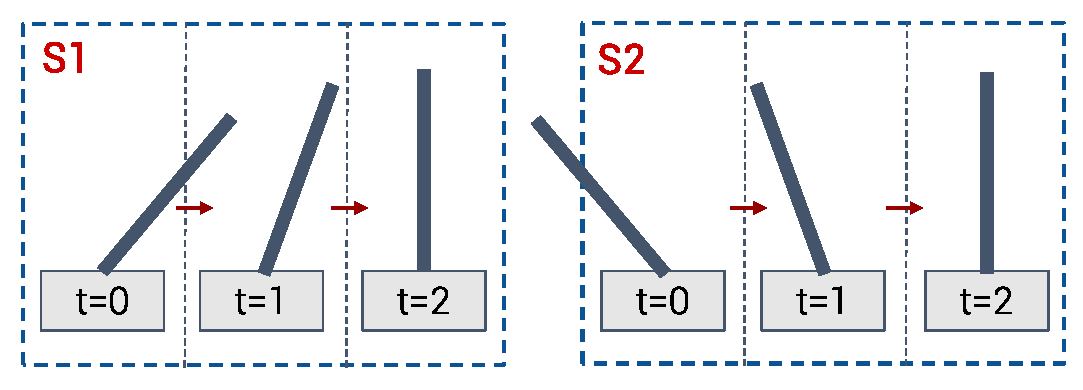
\includegraphics[width=0.9\linewidth]{imagenes/cap4/cartpole_ex.pdf}
    \caption{Cart-pole partial observability example.}
    \label{fig:cp_ex}
\end{figure}

In contrast, if the agent makes decisions based on previous observations it can understand that these two scenarios are different and take better decisions. This is shown in the blue curve of Figure \ref{fig:ld_cartpole_model}, where the agent is able to learn a well performing policy in about 12 minutes. 

\subsection{Validation High-Dimensional State}
In this section we validate D-COACH MON in two different problems (once again, the simulated teacher training strategy introduced in Chapter 3 is used). Cart-pole is a problem that was not originally designed to be solved using as input raw pixels of an image, so we do not expect to obtain a perfect performance. The main goal of testing D-COACH with this problem is to observe if the proposed model (autoencoder + LSTM) is able to embed both the past and high-dimensional inputs adequately.

\begin{figure}[H]
    \centering
    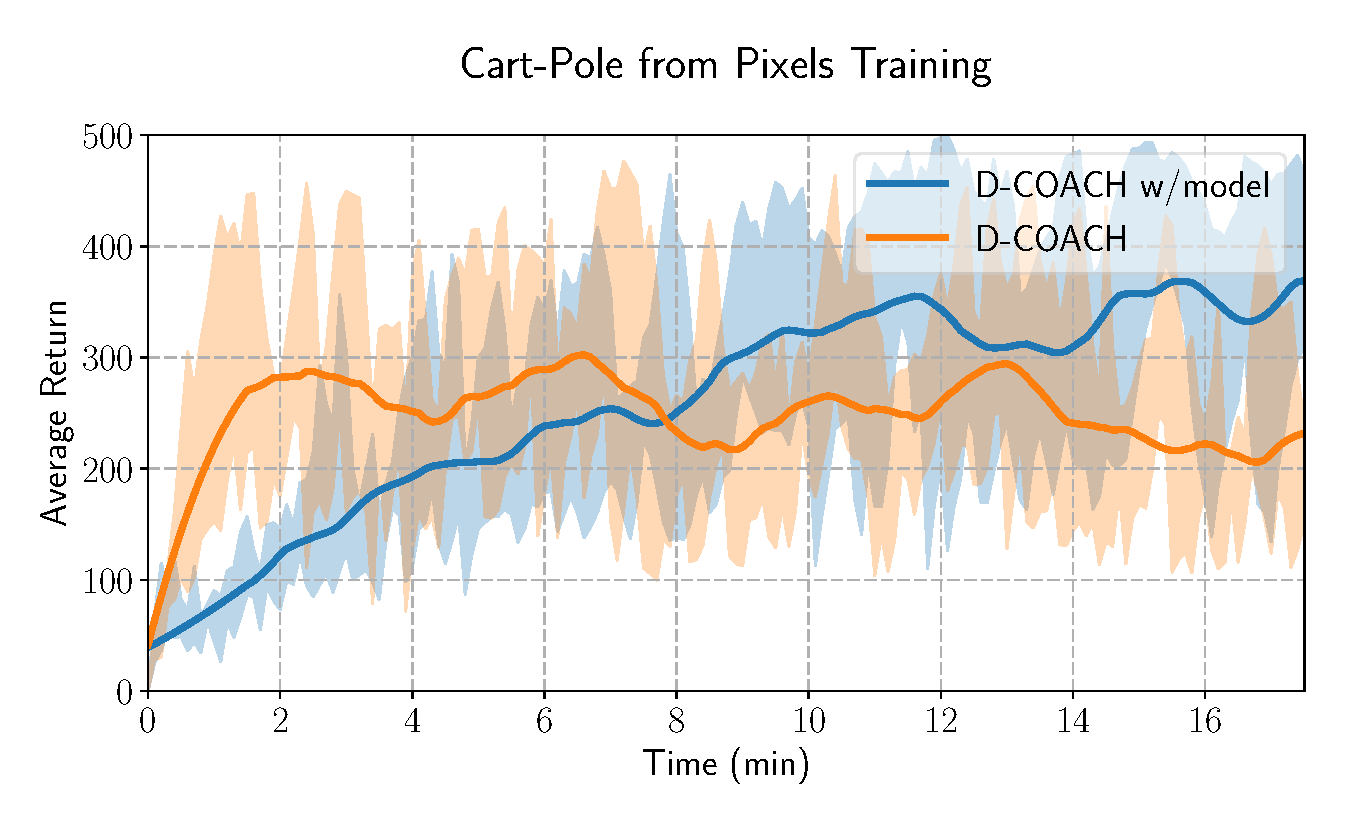
\includegraphics[width=0.8\linewidth]{imagenes/cap3/cartpole_HD_model.pdf}
    \caption{Partially observed cart-pole from pixels results for simulated teacher comparing D-COACH ON and D-COACH MON.  Buffer: $K = 1000$; $k=20$; $b = 1$; $N = 20$; $L=1\mathrm{e}5$; $l=20$; $d=1$; $M=50$; $\tau=4$; $P_{h}$: $\alpha = 0.3$; $\tau = 0.000015$; $\emph{e}=\textbf{1}$; $m=50$; $\epsilon=0.0011$. Simulated teacher network learning rate: $0.0003$; Transition model learning rate: $0.0005$; Autoencoder learning rate: $0.0003$.}
    \label{fig:cp_hd}
\end{figure}

Figure \ref{fig:cp_hd} shows a much more slower learning speed if we compare these agents with the ones of Figure \ref{fig:ld_cartpole_model}. This is expected, since in this case the agents are also learning to extract features from the image. Also, D-COACH ON shows a faster learning speed at the beginning, but after 8 minutes of learning it is outperformed by D-COACH MON. This shows that D-COACH takes longer to learn a temporal/spatial embedding than just a spatial embedding. But, in POMDPs, eventually, D-COACH MON should outperform D-COACH ON.

Finally, D-COACH MON was validated in the partially observed Car Racing problem. Figure \ref{fig:po_cr} shows that D-COACH ON (orange curve) is able to learn a policy that achieves an average return of $\sim700$ after $\sim15$ minutes of training, which is an acceptable score for this problem. Nevertheless, D-COACH MON (blue curve) shows that it is possible to obtain an even better performance if memory is added to the neural network, achieving an average return of $\sim800$ after $\sim15$ minutes of training, which is similar to the performance of $\text{D-COACH}$ ON in the fully observable Car Racing (see Figure \ref{fig:simulatedteachers}). The difference between both curves shows that D-COACH MON is a more robust and powerful approach than $\text{D-COACH}$ ON, capable of enhancing the performance of the agent in problems where $\text{D-COACH}$ ON could appear to be sufficient.

\begin{figure}[h]
    \centering
    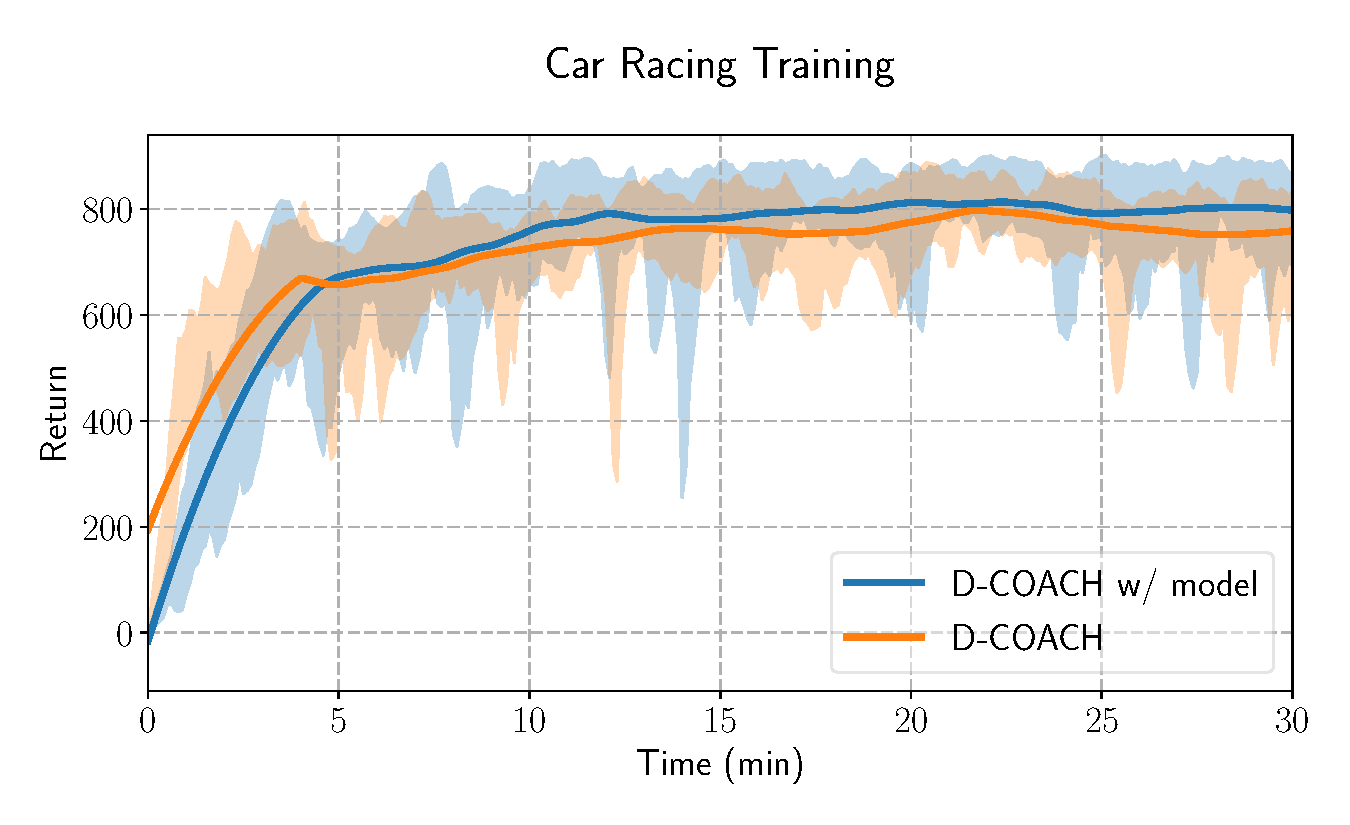
\includegraphics[width=0.8\linewidth]{imagenes/cap3/car_racing_lstm.pdf}
    \caption{Partially observed car racing results for simulated teacher comparing D-COACH ON and D-COACH MON.  Buffer: $K = 2000$; $k=20$; $b=10$; $N = 8$; $L=1\mathrm{e}5$; $l=20$; $d=1$; $M=8$; $\tau=10$; $P_{h}$: $\alpha = 0.9$; $\tau = 0.000015$; $\emph{e}=\textbf{1}$; $m=50$; $\epsilon=0.0011$. Simulated teacher network learning rate: $0.003$; Transition model learning rate: $0.0005$; Autoencoder learning rate: $0.003$.}
    \label{fig:po_cr}
\end{figure}

\section{Discussion}
In this chapter we introduced a variation of D-COACH with memory, D-COACH MON. The main objective was to extend D-COACH in order for it to work in the set of POMDPs where the state is described by time-dependent phenomena. Low-dimensional and high-dimensional problems were covered, introducing a different model architecture for each case. 

D-COACH MON offers a framework that learns both the policy and the model online. This makes it easy for humans to interact in the learning process of the agents, given that no human effort is needed in extra learning steps as in the offline state representation learning version of D-COACH (Chapter 3). The experiments show that the proposed method is effective for enhancing the performance of agents in POMDPs. As discussed previously, memory-based approaches may be key to solve problems in real-world scenarios, where is common to face problems with partial observability. 

As it is stated in the overview of this chapter, RNNs have an extra overhead when training, because sequences must be used for updating the weights of the recurrent layers. Given that D-COACH is an IML approach, updates are done in real-time while the teacher is providing feedback. We found that the overhead produced when updating the recurrent layers is too high for running this approach in CPU; thus, a GPU was used. This is a disadvantage with respect to the previously proposed variations of D-COACH, given that those models are able to run in real-time using CPUs. 
\begin{conclusion}
We presented a framework for learning continuous-action policies using corrective feedback to shape DNN policies in high and low dimensional state spaces. This work was inspired in the COrrective Advice Communicated by Humans (COACH) framework, from where two ideas were taken: (1) the use of binary corrective feedback in action spaces for shaping policies, and (2) the use of past corrections to modify the effects of newer ones. In the COACH framework, these ideas were validated in problems with low-dimensional state spaces using linear combination of basis functions (LCBFs) as function approximators. The novelty of this work is that Deep Neural Networks (DNNs) were used instead, combining ideas of the Deep Reinforcement Learning (DRL) era with the ones of COACH, creating Deep COACH (D-COACH). With D-COACH, we showed that by combining Deep Learning with COACH it is possible to extrapolate the ideas of COACH to learn policies in high-dimensional state spaces and in Partially Observable Markov Decision Processes (POMDPs) within the tens of minutes. 

The hypothesis of this thesis was supported with several experiments. We showed that human corrective feedback can be used to learn well performing DNN policies in a time-efficient and reward function free way.

First, D-COACH was validated in a low-dimensional state problem (cart-pole). This is a simple widely-studied problem that is useful to test early versions of sequential decision making learning algorithms. This problem had also been previously solved using COACH, which made it a good candidate to compare the performance of D-COACH with the one of COACH. This experiment showed that D-COACH worked well in low-dimensional state problems and with a performance similar to the one of COACH. 

For high-dimensional state problems, two variations of D-COACH were proposed and compared: online state learning and offline state learning. Both variations obtained similar final performances in the Car Racing and the Duckie Racing problems. The main advantage found in the online state learning version over the offline state version, is that it is an approach that requires less time and effort from the human user. Everything is learned from scratch and interactively, while in the offline state learning case a database of the agent exploring the environment must be obtained and used to train an autoencoder before starting the interactive learning process of the policy. Online state learning D-COACH had an extra validation in a 3DoF arm, where an agent learned to solve the reacher and pusher tasks from scratch.

Finally, a last variation of D-COACH (model-based) for POMDPs in where the observations do not capture time-dependent phenomena from the state was proposed. The approach was to give memory to the agent by adding recurrent layers, LSTMs, to the DNN models. By comparing model-free with model-based D-COACH in low and high dimensional state problems using a simulated teacher, we observed that learning a model of the dynamics of the environment could be crucial in some cases for obtaining well performing policies. Also, that in other cases it may improve the performance of the agent. 

Even though the algorithms proposed in this work were validated and supported the hypothesis of this thesis, we believe that there is still a lot of work and research left to be done in this area. There are some ideas proposed in the COACH framework that we did not study with D-COACH and are worth mentioning:

\begin{itemize}
    \item \textbf{Human Model:} In D-COACH we replaced the Human Model with a replay buffer, as mentioned in Chapter 2. Even though both approaches use information given by past corrections to modify the effects of newer ones, they do not do it in the same way. The Human Model modifies the learning rate of the policy; the replay buffer updates the policy constantly by replaying past corrections. Including a Human Model in D-COACH could help with the dilemma of setting either a too large or too small magnitude of the learning rate when updating the policy with SGD. In this case, we did not include a Human Model because this would have meant to add a second DNN model in charge of learning it. Thus, the overhead of D-COACH would have increased and for a first approach we prioritized a lighter model.
    \item \textbf{Credit assigner:} Module proposed in TAMER approaches \cite{Knox:2009:ISA:1597735.1597738} which COACH adopted. This module associates feedback not only with the last state-action pair, but with past state-action pairs as well. The objective is to characterize the the human delay with a probability that weights correction signals with a sequence of state-action pairs. This could help with the data-efficiency of D-COACH. Nevertheless, given that D-COACH was able to work fine without this module, studying the advantages of adding it to the framework was left for future work. 
    \item \textbf{D-COACH + DRL:} In \cite{celemin2018fast}, a hybrid RL framework with COACH is proposed. The basic idea is to use corrective feedback along with RL algorithms in order to speed up the learning process. The same concept could be applied and studied with D-COACH. 
\end{itemize}

In contrast, the are some shortcomings that D-COACH presents that would be beneficial to study in future research:
\begin{itemize}
    \item \textbf{High-dimensional action spaces:} One of the main shortcomings of D-COACH was inherited from COACH. Both approaches are limited to work in problems with low-dimensional action spaces due to that humans must provide corrections in the action space. If the action space of a problem is too large, then is not intuitive for a human to give feedback, and he/she may not be able to correct the agent. Modules that interpret feedback from a correction space to the agent's action space can be added to tackle this shortcoming, such using inverse kinematics modules. But this is not always possible or trivial to do, so more research in this area could  enhance the capabilities of D-COACH.
    \item \textbf{Experience Replay size:} Given that the size of the replay buffer of D-COACH is limited due to its on-policy nature, it may be challenging (or not possible) to solve problems that require more complex decision-making strategies that the ones tested in this thesis. This is because in more complex scenarios, agents may need to store corrections in memory for a longer time than what the buffer is able to do, due to its limited size. Thus, valuable corrections would be forgotten, affecting the performance of the agent. Developing strategies to overcame this limitation could be key for using D-COACH in more complex settings. 
\end{itemize}

Beyond the limitations of D-COACH and the future research that can be done in this area, the variations of D-COACH presented in this work showed to be a valid alternative for teaching robots to solve sequential decision-making problems using DNN policies. Human teachers were able to interact with real-world platforms (Duckie Racing and 3DoF arm) and guide them through the learning process for solving tasks.
\end{conclusion}


\nocite{*}
\newpage
\addcontentsline{toc}{chapter}{\protect\numberline{}Bibliography}
\bibliographystyle{plain}
\bibliography{bibliography}

\begin{appendix2}
\section*{Publications}
Throughout the development of this thesis two conference papers were written and accepted:

\begin{itemize}
    \item R. Pérez-Dattari, C. Celemin, J. Ruiz-del-Solar, J. Kober. ``Continuous Control for High-Dimensional State Spaces: An Interactive Learning Approach". International Conference on Robotics and Automation \textbf{(ICRA)}. (2019)
    \newline\color{blue}\textbf{Paper available:} \color{black} \url{www.jenskober.de/publications/PerezDattariICRA2019.pdf}
    
    \vspace{0.5cm}
    
    \item R. Pérez-Dattari, C. Celemin, J. Ruiz-del-Solar, J. Kober. ``Interactive Learning with Corrective Feedback for Policies based on Deep Neural Networks". International Symposium on Experimental Robotics \textbf{(ISER)}. (2018)
    \newline\color{blue}\textbf{Paper available:} \color{black} \url{www.arxiv.org/abs/1810.00466}
\end{itemize}

The ISER paper was done with the work present in Chapter 3; the ICRA paper was done with the work present in Chapter 4. In both cases the code was made public through the github platform:

\begin{itemize}
    \item \textbf{ICRA code:} \url{git.io/fjv2e}
    
    \vspace{0.5cm}
    
    \item \textbf{ISER code:} \url{git.io/fxA3x}
\end{itemize}
\end{appendix2}
\end{document}